\documentclass[a4paper, twoside]{report}

%% Language and font encodings
\usepackage[english]{babel}
\usepackage[utf8x]{inputenc}
\usepackage[T1]{fontenc}
\usepackage{enumitem}

%% Sets page size and margins
\usepackage[a4paper,top=3cm,bottom=2cm,left=3cm,right=3cm,marginparwidth=1.75cm]{geometry}

%% Useful packages
\usepackage{amsmath}
\usepackage{graphicx}
\usepackage[colorinlistoftodos]{todonotes}
\usepackage[colorlinks=true, allcolors=blue]{hyperref}

%% own packages
\usepackage{xcolor}
\usepackage{subcaption}
\usepackage{amsmath}
\usepackage{gensymb}
\usepackage{amssymb}
\usepackage{algorithm}
\usepackage{algorithmicx}
\usepackage[noend]{algpseudocode}
\usepackage{booktabs}
\usepackage[titletoc]{appendix}
\usepackage{titlesec}
\usepackage{listings}
\usepackage{enumitem}
\usepackage{multirow}
\usepackage{placeins}
\usepackage{rotating}
\usepackage{pifont}
\usepackage{array}
\usepackage{mdframed}
\usepackage{lipsum}
\usepackage[utf8]{inputenc}
\usepackage[many]{tcolorbox}
\usepackage{varwidth}
\usepackage{cleveref}
\usepackage{colortbl}
\usepackage{array}
%\usepackage{breqn}

%% own settings
% article
\setlength{\parindent}{0pt}
\setcounter{secnumdepth}{3}
\setcounter{tocdepth}{3}
% remove Chapter number from header name
%\titleformat{\chapter}[display]
%  {\normalfont\bfseries}{}{0pt}{\Huge}

\setlist{nosep}
\setlist{nolistsep}
\setlist{topsep=-5px}

\def \hfillx {\hspace*{-\textwidth} \hfill}

\makeatletter
\newcommand*{\centerfloat}{%
  \parindent \z@
  \leftskip \z@ \@plus 1fil \@minus \textwidth
  \rightskip\leftskip
  \parfillskip \z@skip}
\makeatother

\newcommand{\cmark}{\ding{51}}%
\newcommand{\xmark}{\ding{55}}%

\newcolumntype{P}[1]{>{\centering\arraybackslash}p{#1}}
\newcolumntype{M}[1]{>{\centering\arraybackslash}m{#1}}

\newenvironment{tight_enumerate}{
\begin{enumerate}
  \setlength{\itemsep}{0pt}
  \setlength{\parskip}{0pt}
}{\end{enumerate}}

% math
\newcommand{\norm}[1]{\left\lVert#1\right\rVert}
\newcommand{\argmax}[2]{\underset{#1}{\arg \max} \hspace{0.1cm} #2}
\newcommand{\argmin}[2]{\underset{#1}{\arg \min} \hspace{0.1cm} #2}

\newmdtheoremenv{theo}{Theorem}
\newmdtheoremenv{proof}{Proof}

% Theo
\tcbuselibrary{theorems}
\newtcbtheorem[number within=chapter, crefname={theorem}{theorems},Crefname={Theorem}{Theorems}]{Theo}{Theorem}%
%
{enhanced, frame empty, interior empty, arc=0mm,
coltitle=black, fonttitle=\bfseries, colbacktitle=white,
borderline={0.5mm}{0mm}{},%
attach boxed title to top center={yshift=\dimexpr-\tcboxedtitleheight/2},
boxed title style={boxrule=-1pt},varwidth boxed title,
fontupper=\itshape, }{Th}

\newtcbtheorem[no counter, crefname={proof}{Proofs},Crefname={Proof}{Proofs}]{Proof}{Proof}%
%
{enhanced, frame empty, interior empty, arc=0mm,
coltitle=black, fonttitle=\bfseries, colbacktitle=white,
borderline={0.5mm}{0mm}{},%
attach boxed title to top center={yshift=\dimexpr-\tcboxedtitleheight/2},
boxed title style={boxrule=-1pt},varwidth boxed title,
fontupper=\itshape, }{Pf}

\title{Global Way-point LSTM Planner: An Online Machine Learning Solution for Robotic Path Planning}
\author{Alexandru Iosif Toma}
% Update supervisor and other title stuff in title/title.tex

\begin{document}
\begin{titlepage}

\newcommand{\HRule}{\rule{\linewidth}{0.5mm}} % Defines a new command for the horizontal lines, change thickness here

%----------------------------------------------------------------------------------------
%	LOGO SECTION
%----------------------------------------------------------------------------------------


\includegraphics[width=8cm]{title/logo.png} \vspace{1.3cm} % Include a department/university logo - this will require the graphicx package
 
%----------------------------------------------------------------------------------------

\center % Center everything on the page

%----------------------------------------------------------------------------------------
%	HEADING SECTIONS
%----------------------------------------------------------------------------------------

\textsc{\LARGE MEng Individual Project}\\[1.5cm] % Name of your university/college
\textsc{\Large Imperial College London}\\[0.5cm] % Major heading such as course name
\textsc{\large Department of Computing}\\[0.5cm] % Minor heading such as course title

%----------------------------------------------------------------------------------------
%	TITLE SECTION
%----------------------------------------------------------------------------------------
\makeatletter
\HRule \\[0.4cm]
{ \huge \bfseries \@title}\\[0.4cm] % Title of your document
\HRule \\[1.5cm]
 
%----------------------------------------------------------------------------------------
%	AUTHOR SECTION
%----------------------------------------------------------------------------------------

\begin{minipage}{0.4\textwidth}
\begin{flushleft} \large
\emph{Author:}\\
\@author % Your name
\end{flushleft}
\end{minipage}
~
\begin{minipage}{0.4\textwidth}
\begin{flushright} \large
\emph{Supervisor:} \\
Sajad Saeedi \\[1.2em] % Supervisor's Name
\emph{Co-supervisor:} \\
Ronald Clark \\[1.2em]
\emph{Second Marker:} \\
% second marker's name
Andrew Davison \\[1.2em]

\end{flushright}
\end{minipage}\\[2cm]
\makeatother

% If you don't want a supervisor, uncomment the two lines below and remove the section above
%\Large \emph{Author:}\\
%John \textsc{Smith}\\[3cm] % Your name

%----------------------------------------------------------------------------------------
%	DATE SECTION
%----------------------------------------------------------------------------------------

{\large \today}\\[2cm] % Date, change the \today to a set date if you want to be precise

\vfill % Fill the rest of the page with whitespace

\end{titlepage}

\newpage
\mbox{}
\newpage

\begin{abstract}

%The path planning problem has essential applications in physical autonomous systems, such as robots and self-driving cars. 
Path planners have indispensable applications in physical autonomous systems such as robots and self-driving cars, in which human intervention is not desirable: bomb defusing, search and rescue, large scale manufacturing, warehouse management and many more. However, some of the classic solutions satisfy only a subset of the real-world application requirements imposed by hardware limitations. The work from this report shows that by adopting a hybrid approach between classic solutions and Machine Learning methods, we can develop a path planning solution that has support for partial knowledge environments while theoretically satisfying the real-world constraints. We create a platform for testing and developing the proposed solution while offering support for \textit{ROS}, a defacto in robotic systems. We theoretically and empirically assess the performance of the proposed solution against the well-known pathfinding solution, A*. We prove that the proposed solution achieves theoretically lower average case time and space complexity and significantly reduces the memory load compared to A*. Moreover, we show that the proposed solution is robust to unknown environments by evaluating it on real-world occupancy grid maps. Lastly, we run the proposed solution on a real-world robot and show that it can find a reasonable path in partial knowledge environments in which offline solutions such as A* cannot.

%The work from this report showcases a new hybrid pathfinding algorithm between classic solutions and ML methods, the Global Way-point LSTM Planner.

%

\end{abstract}

\renewcommand{\abstractname}{Acknowledgements}
\begin{abstract}

I would like to thank my supervisor, Sajad Saeedi for offering continuous support and invaluable advice in regards to the project. I would like to thank my co-supervisor, Ronald Clark for motivating me to pursue different objectives. I would like to thank my second marker, Andrew Davison for inspiring me to address real-world robotic applications in the Interim Report. I would like to thank the Percepbot team for offering me the robot hardware for the real-world evaluation. I would like to thank my friends, Alexandru Dan and Andrei Isaila for proof-reading my report. Lastly, I would like to thank my parents and all my friends for their emotional support during my university years.

\end{abstract}

{
  \hypersetup{hidelinks}
  \tableofcontents
}
%\listoffigures %85
%\listoftables  %53

\setlength{\parskip}{\baselineskip}
% \chapter{Introduction}
% The path planning problem is an important application in autonomous systems such as robots and self driving cars \cite{inoue2019robot, gonzalez2016review}. Due to the fact that, nowadays, most physical autonomous systems tasks involve movement from point A to B, it is crucial to find an efficient solution for this problem. As a consequence, we would like to create a path planning decision making algorithm that would plan the journey in such a way that the robot will not collide with any obstacles \cite{gonzalez2016review} in an efficient way.

% But, what is an efficient path planning algorithm? An efficient decision process can refer to multiple aspects such as finding the optimal solution in terms of distance (i.e. shortest distance), most energy efficient solution (robots might have an energy aspect associated with them such as velocity, acceleration, traction power, torque speed that consumes a substantial portion of the battery life) and computational cost (in the real world robots need to process the terrain and take decisions at each point in time, if the algorithm is really slow it could not even reach the destination especially if the environment is constantly moving) \cite{gonzalez2016review}.

% The aim of the paper is to develop such a decision algorithm by using an LSTM \cite{hochreiter1997long} (Long short-term memory) recurrent neural network and compare it to the previous works \cite{nicola2018lstm, lee2018lstm, inoue2019robot}. But in order to correctly asses the performance of the algorithm we need to review the current existing solutions and compare our results against them as well.

% \section{Motivation}
% In the \hyperref[LiteratureReview]{Literature Review} section we are going to study the current available solutions to the path finding problem and the first thing that we are going to notice is that there are a lot of them (not including variations). So why would we bother creating a new algorithm when so many good solutions exist already?

% %\subsection{Importance}
% % - why does it matter
% % - include example, bomb defusing, warehouses Amazon
% % - should be fast, quality
% % - technical aspects
% % - advantages of NN over classic algorithms (uncertainty)
% % - technical objectives
% % - move from A to B

% \section{Proposed method}
% % - talk about the LSTM solution
% The reason of choosing the LSTM approach is because the path planning algorithm can be described as a sequential problem and the LSTM is build with the purpose of solving this kind of problems.

% %\subsection{Significance}
% % - high level (general)
% % - more subjective
% % - repeat importance, but high level

% \section{Outline}
% % - report chapters summarised (2-3)

% \section{Methodology}
% % - how I am going to solve it
% % - image map
% % - network
% % - map generation: game of life

\chapter{Introduction}

Path planners have essential applications in physical autonomous systems, such as robots and self-driving cars, as they have to safely follow an efficient, collision-free trajectory to their destination \cite{inoue2019robot, gonzalez2016review}. Nowadays, autonomous systems are indispensable, their purpose being, the automation of tasks that cannot be performed at large scale or in a safe manner by a human being. Some examples include military applications (e.g. bomb-defusing robots), search-and-rescue robots, large scale manufacturing robots and warehouses management robots \cite{inoue2019robot}. As a consequence, it is crucial to develop an efficient path planning algorithm that would plan a safe journey for the robot \cite{gonzalez2016review}.

We argue that in real-world path planning, the robots interact with the real world environment and thus are subject to physical constraints. Therefore, the path planning decision algorithm has to satisfy various requirements imposed by hardware limitations \cite{lavalle2001randomized}: 

\begin{itemize}
    \item \textbf{Resource Load} - The solution has to be computationally and memory efficient by taking into account the hardware limitations imposed by the robot architecture
    \item \textbf{Partial Knowledge (Online Planners)} - Usually in robotics, the planner has to find a solution with partial knowledge about the map. Thus, the algorithm has to explore the map while searching for a solution (i.e. the algorithm becomes online; e.g. a robot with a SLAM sensor has only localised information, until more areas are discovered)
    \item \textbf{Dynamic Environments} - The real world is highly dynamic and local path planning algorithms should support real-time path generation and collision detection
    \item \textbf{Robustness to Unknown Environments} - The solution should generalise well in unknown environments by preserving all other constraints
    \item \textbf{Non-holonomic Constraints} - Most robots (e.g. self-driving cars) do not possess the ability to move in all available degrees of freedom instantaneously. Therefore, the solution should plan a trajectory that can be followed with maximal efficiency (e.g. a car has to follow a curved path when turning to the left or right). Lastly, the path should also take into consideration the available physical capabilities of the robot (e.g. a robot has limited manoeuvring)
    \item \textbf{Randomized Kinodynamic Planning} - Path planners should generate a path based on the imposed vehicle constraints such as velocity, acceleration and torque. Therefore, we can avoid collisions with obstacles due to high velocity
    \item \textbf{Higher Dimensional Scaling (3D)} - The solution should be easily and feasibly extended to robots with higher degrees of freedom (e.g. drones and flying robots)
\end{itemize}

% real world applications in industry, dynamic environments, robustness, randomized kinodynamic planning, non-holonomic constraints, higher dimensional scaling (3D) and resource load.

% Move in significance
%Nowadays, autonomous systems are indispensable and they serve as purpose, the automation of tasks that can't be performed at large scale or in a safe manner by a human being. Some examples include military applications (e.g. bomb defusing robots), search-and-rescue robots, large scale manufacturing robots and warehouses management robots. As a consequence, it is crucial to develop an efficient path planning decision making algorithm that would plan a safe journey for the robot \cite{gonzalez2016review}.

% But, what is an efficient path planning algorithm? An efficient decision process can refer to multiple aspects such as finding the optimal solution in terms of distance (i.e. shortest distance), most energy efficient solution (robots might have an energy aspect associated with them such as velocity, acceleration, traction power, torque speed that consumes a substantial portion of the battery life) and computational cost (in the real world robots need to process the terrain and take decisions at each point in time, if the algorithm is really slow it might not even reach the destination especially if the environment is constantly moving) \cite{gonzalez2016review}.

Currently, there are a lot of classic solutions to the pathfinding problem. To mention some of the most important ones: A* \cite{choset2005principles, duchovn2014path, zhang2014multiple, 5937169}, Rapidly-exploring Random Tree (RRT) family \cite{lavalle1998rapidly, rodriguez2006obstacle, lavalle2001randomized, karaman2011sampling}, Value Iteration on Markovian Decision Processes (MDP) \cite{szepesvari2010algorithms, satia1973markovian}. However, most of the classic algorithms are computationally expensive because they have to search a vast area. A* and Informed RRT* are pruning the search space by adopting a heuristic function $h$ (e.g. the Euclidean distance between the agent and the goal or the ellipsoid heuristic respectively), but even so, if the environment is complex (e.g. contains unusually shaped obstacles, the path is meandering), the search is not pruned enough. Moreover, the computational cost and memory increase exponentially with the dimension of the environment. Additionally, there exist environments (e.g. maps without a metric space such as networks) where finding a proper heuristic function is not trivial. Lastly, most of the classic algorithms are offline, and thus, they require full knowledge about the map.

\section{Objective}

This project aims to investigate if Machine Learning (ML) methods are a viable option for path planning applications. We will attempt to develop a ML solution that solves the path planning problem while satisfying the real world industrial applications requirements. We are going to focus mainly on the partial knowledge, resource load reduction (memory efficiency; See Figure \ref{fig: intro_show}) and robustness to unknown environments properties by running empirical evaluations while only theoretically prove the others.

The proposed solution will be developed using an LSTM \cite{hochreiter1997long} (Long Short-Term Memory) recurrent neural network architecture. The motivation behind choosing an LSTM architecture is derived by the fact that the path planning algorithm can be described as a sequential problem and it has been proved that LSTMs produce excellent results in this area (e.g. speech recognition, time series, anomaly detection, text generation, machine translation and many more) \cite{Goodfellow-et-al-2016}. There has been some work done with LSTMs \cite{nicola2018lstm, lee2018lstm, inoue2019robot} in this field, but their approach had a low success rate of finding a path to the goal (even if one exists). Therefore, we will attempt to boost the success rate by creating hybrid solutions between pure ML solutions and classic solutions such as A*.

In order to achieve the objectives mentioned above, we are going to use a simulation platform. Currently, there are a variety of standardised motion planning libraries such as: \textit{ROS} \cite{Quigley09}, \textit{OMPL} \cite{sucan2012the_open_motion_planning_library}, \textit{MoveIt} \cite{moveit} (which has benchmarking capabilities \cite{moll2015benchmarking}). However, we are going to build our development platform, PathBench. The main reason behind this choice is that we are going to focus on the actual generation of the path instead of the physical interactions between the robot and the environment. Thus, we boost development productivity while focusing on the key components of the solution. Furthermore, by creating standardised APIs, we can easily port the path planners to the specified libraries. Finally, we need training data, a ML pipeline and a benchmarking module which the current libraries do not provide.

\begin{figure}[h!]
  \centering
  \begin{subfigure}[b]{0.32\linewidth}
    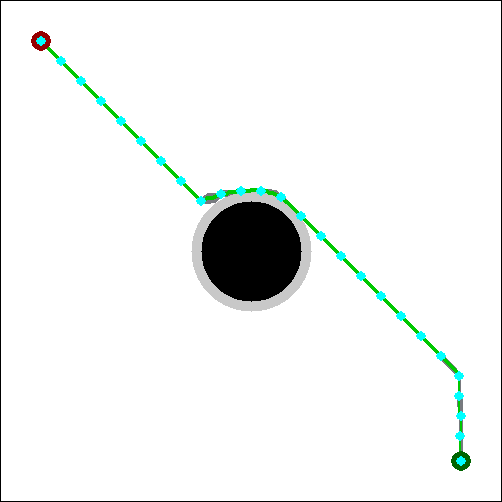
\includegraphics[width=\linewidth]{images/screenshot_51.png}
    \caption{Global Way-point LSTM Planner (proposed solution)}
  \end{subfigure}
  \hspace{2cm}
  \begin{subfigure}[b]{0.32\linewidth}
    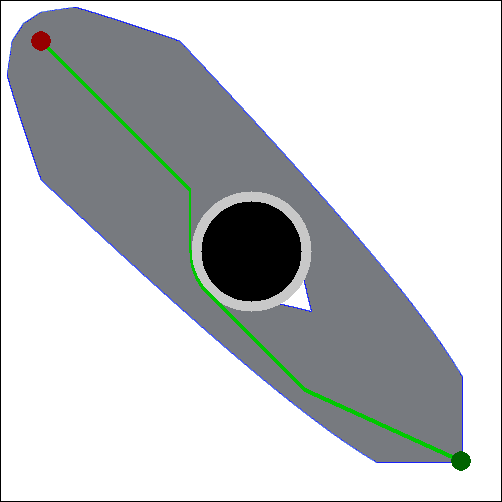
\includegraphics[width=\linewidth]{images/screenshot_44.png}
    \caption{A* \newline}
  \end{subfigure}
  \caption{Memory load comparison between the Global Way-point LSTM Planner (proposed solution) and A*. The red circle represents the agent (robot) position, the green circle represents the goal position and the black/light-grey regions represent obstacles. The dark grey regions represent the total search space used by the respective algorithms}
  \label{fig: intro_show}
\end{figure}

\pagebreak

% Tare goinhe aiuse a simulation platform. Currently, there are a variety of m, g to we  of the report, is to develop a pruning algorithm that will speed up a classic algorithm such as A* or Informed RRT* by reducing the search space.

% Having this in mind, we are going to use an LSTM \cite{hochreiter1997long} (Long short-term memory) recurrent neural network architecture to implement the above mentioned procedure by using A* as ground truth. There has been some work done with LSTMs \cite{nicola2018lstm, lee2018lstm, inoue2019robot}, but their approach was to use LSTMs to \textbf{produce} an actual path. One of the major disadvantages of using this method, is that the robot will not always succeed in finding the goal, even if there \textbf{exists} a solution \cite{nicola2018lstm}. Therefore, we introduce the idea of probabilistic search space, in order to make sure that the algorithm will eventually find a path.

% The reason of choosing an LSTM architecture is derived by the fact that the path planning algorithm can be described as a sequential problem and it has been proved that LSTMs produce great results in this area (e.g. speech recognition, time series anomaly detection, text generation and many more).

% Moreover, by using a machine learning approach we should solve the problem of finding a good heuristic function in complex environments.

%\section{Significance}
%We argue that in real world path planning, the robots interact with the real world environment and thus are subject to physical constraints. Therefore, we attempt to develop a solution that solves some of the following areas: real world applications in industry, dynamic environments, robustness, randomized kinodynamic planning, non-holonomic constraints, higher dimensional scaling (3D) and resource load.

%\todo{Complete this section}

%In order to devise an extension for a current solution, we first need to study the current available classic algorithms which are eligible with this kind of extension. We will also cover the non-eligible algorithms as a comparison standard. The \hyperref[LiteratureReview]{Literature Review} section presents the most popular classic path finding algorithms.

%In the \hyperref[Background]{Background} section, we are going to review the machine learning architectures and principles needed in the development of the proposed solution.

%In the \hyperref[Solution]{Solution} section, we are going to state our proposed solution by exemplifying the machine learning architecture that we have used and the algorithm itself.

%In the \hyperref[Simulator]{Simulator} section, we are going to discuss about our simulation environment where we will be testing the proposed solution and generate the training data.

%In the \hyperref[Evaluation]{Evaluation} section, we are going to asses the performance of the proposed solution against the studied algorithms.

%In the \hyperref[Conclusion]{Conclusion} section, we are going to summarise our findings and address future work.

\section{Contributions}

The contributions of this report include (the source code can be found at \url{https://gitlab.doc.ic.ac.uk/ait15/individual-project}): 

\begin{itemize}
    \item Three algorithmic contributions: \begin{itemize}
        \item \textbf{CAE Online LSTM Planner} - The first proposed solution, Online LSTM Planner, is almost identical to the paper implementation from \cite{nicola2018lstm} with different input selection and the addition of a max iterations argument. The CAE Online LSTM Planner is a hybrid solution between \cite{nicola2018lstm} and \cite{inoue2019robot}. The Convolutional Auto-encoder (CAE) architecture was built by us, and the LSTM architecture was borrowed from \cite{nicola2018lstm}
        \item \textbf{LSTM Bagging Planner} - This algorithm is inspired by ensemble learning solutions, and it is used to boost the performance of the Online LSTM and CAE Online LSTM Planners
        \item \textbf{Global Way-point LSTM Planner} - The final proposed solution uses the LSTM Bagging Planner to create a global way-point suggestion algorithm. It has nice flexibility properties, significantly reduced memory load compared to A*, support for partial knowledge environments, robustness to unknown environments and a theoretically lower average case time and space complexity compared to A*
    \end{itemize}
    \item PathBench - A benchmarking platform for classic and learned path planning algorithms with the following four main components and extension: 
    \begin{itemize}
        \item \textbf{Simulator} - We have built a simulator as a practical way of visualising the behaviour of the path planners. It includes different features such as animations, control for animations (stop, resume), custom displays for individual algorithms and it is highly extensible to support new solutions
        \item \textbf{Generator} - The generator was build to acquire training data for our ML solutions. It can generate three types of maps: uniform random fill maps, block maps and house maps. It can also be extended to include more synthetically generated data (e.g. cellular automata cave generation and maze generation) as well as convert real-world datasets (e.g. Simultaneous Localisation and Mapping (SLAM) images \cite{dissanayake2001solution}) into internal simulator environments. All maps can be converted into training datasets which contain a variety of features and labels generated using A* as ground truth
        \item \textbf{Trainer} - We have built a training environment to boost the productivity of testing new ML architectures. It has an automatic pipeline for extracting a subset of the generated training data and caching subroutines to increase the speed of second runs
        \item \textbf{Analyser} - We have developed an analyser tool to assess the performance of the proposed algorithms against classical solutions such as A*. The analyser contains multiple assessment routines which stress the performance of the tested algorithms in multiple areas (e.g. speed, efficiency and memory)
        \item \textbf{ROS Real-time Extension} - We have added support for real-world simulation by implementing an updatable map environment which is compatible with the \textit{gmapping} \textit{ROS} package (i.e. SLAM scan)
    \end{itemize}
    \item Theoretic and real-world evaluations performed as follows: \begin{itemize}
        \item \textbf{Complexity and Theoretical Analysis} - For each proposed solution, we have theoretically proven the worst case time and space complexity. Moreover, we have discussed the worst case time and space complexity of higher dimensional scaling. Lastly, we have proved that the proposed solution achieves theoretically lower average case time and space complexity compared to A*
        \item \textbf{Empirical Methods} - We have created specific statistical metrics for each proposed solution. The metrics are used to gain insight into the general behaviour of the proposed solutions and their real-world applications effectiveness. We have showed that the proposed solution significantly reduces the memory load compared to A* (See Figure \ref{fig: intro_show}) and that it generalises well in unknown environments
        \item \textbf{Real-world Evaluation} - We have tested the performance of the proposed solution on real-world occupancy grid maps generated by real-world robots. Furthermore, we have implemented the proposed solution on a real-world robot and tested it at Imperial College London. We have proved that the proposed solution is applicable in real-world scenarios. Moreover, we have proved the partial knowledge property by showing that the algorithm can run in environments with partial information in which some classic offline algorithms such as A* are unable to find a solution
    \end{itemize}
\end{itemize}

\section{Report Outline}
%\textbf{\hyperref[LiteratureReview]{Literature Review}.}
%\paragparh{Chapter \ref{LiteratureReview} (\hyperref[LiteratureReview]{Literature Review}).}
\paragparh{\hyperref[LiteratureReview]{Literature Review} (Chapter \ref{LiteratureReview}).} In this chapter, we will study the current path planning solutions by categorising them into separate sections based on the type of planner. We will assess the optimality conditions, give a brief time and space complexity analysis, study the structure of the algorithms and state the advantages and disadvantages of each solution.

% \textbf{\hyperref[Background]{Background}.}
%\paragparh{Chapter \ref{Background} (\hyperref[Background]{Background}).}
\paragparh{\hyperref[Background]{Background} (Chapter \ref{Background}).} The Background Chapter will cover the basics of ML and explain the structure of the LSTM network. We will discuss data pre-processing, training routines, evaluation methods and hyper-parameter tuning.

% PathBench
% MLWP Planner
% capital section

%\textbf{\hyperref[Simulation Platform]{Simulation Platform}.} 
%\paragparh{Chapter \ref{Simulation Platform} (\hyperref[Simulation Platform]{Simulation Platform}).} 
\paragparh{\hyperref[Simulation Platform]{PathBench} (Chapter \ref{Simulation Platform}).} In this chapter, we are going to describe PathBench, the platform used to develop and test the classic and proposed solutions. We will cover the architecture design of all platform components and explain the current capabilities and limitations by comparing it to the standard motion planning libraries.

%\textbf{\hyperref[sec: methods]{Methods}.}
%\paragparh{Chapter \ref{sec: methods} (\hyperref[sec: methods]{Methods}).}
\paragparh{\hyperref[sec: methods]{Methods} (Chapter \ref{sec: methods}).} In this section, we are going to describe the proposed solutions by following the same investigations as in Chapter \ref{LiteratureReview} (\hyperref[LiteratureReview]{Literature Review}). Moreover, we will compare the theoretical performance against the well-known algorithm A* by giving a thorough time and space complexity analysis for all proposed solutions.

%\textbf{\hyperref[Evaluation]{Evaluation}.} 
%\paragparh{Chapter \ref{Evaluation} (\hyperref[Evaluation]{Evaluation}).} 
\paragparh{\hyperref[Evaluation]{Evaluation} (Chapter \ref{Evaluation}).} In this chapter, we are going to run a series of empirical evaluation routines which will stress the proposed solution performance. We are going to examine each empirical run and give a theoretical interpretation of the results. Moreover, we will test the performance of the path planner on real-world occupancy grid maps produced by real-world robots. Lastly, we will run the proposed solution on a real robot at Imperial College London and assess its performance.

%\textbf{\hyperref[Conclusion]{Conclusion}.} 
%\paragparh{Chapter \ref{Conclusion} (\hyperref[Conclusion]{Conclusion}).} 
\paragparh{\hyperref[Conclusion]{Conclusion} (Chapter \ref{Conclusion}).} In the final chapter, we are going to summarise our findings and address future work.
\chapter{Literature Review} \label{LiteratureReview}
We are going to divide the classic algorithms into four sections following the model from \cite{gonzalez2016review}: \hyperref[A. Graph search planners]{Graph Search Planners} (Section \ref{A. Graph search planners}), \hyperref[B. Sampling based planners]{Sampling Based Planners} (Section \ref{B. Sampling based planners}), \hyperref[C. Interpolating curve planners]{Interpolating Curve Planners} (Section \ref{C. Interpolating curve planners}), \hyperref[D. Numerical optimization approaches]{Numerical Optimization Approaches} (Section \ref{D. Numerical optimization approaches}).
%\begin{enumerate}[label=\Alph*.]
%    \item \hyperref[A. Graph search planners]{Graph search planners}
%    \item \hyperref[B. Sampling based planners]{Sampling based planners}
%    \item \hyperref[C. Interpolating curve planners]{Interpolating curve planners}
%    \item \hyperref[D. Numerical optimization approaches]{Numerical optimization approaches}.
%\end{enumerate}

When discussing each algorithm, we are going to state how it solves the problem, how it is implemented, optimality conditions, worst case time and space complexity analysis and some of the advantages and disadvantages.

%When discussing about each algorithm we are going to describe each solution by stating how it solves the problem and state some of the advantages or disadvantages. %if it is an efficient solution (optimality, energy efficiency, computational cost). %At the end of the \hyperref[LiteratureReview]{Literature Review} section we are going to compare the performance of all algorithms.

However, before starting, let us quickly formalise the pathfinding problem so that we will have a standard notation throughout the review. We have an agent $A$ that wants to get to a goal $G$ and a set of obstacles $Os$ which the agent tries to avoid. Each of the entities belongs to a map $M=(A, Os, G)$. The purpose of the algorithm is to produce a trace, denoted by $T$, which represents the history of the agent moves from the initial agent position to the goal position. The agent can move one step at a time to a position that is valid within the map (not out of bounds or not colliding with any obstacles). The goal is reached by the agent only when the agent position matches the goal position exactly. Furthermore, we are going to assume that the environment is static and fully discovered (the algorithm does not need to explore the map while searching for a solution).

As a general rule, when we inspect the map figures, the entities will be represented by circles or squares. The colour convention will be the following: the agent is red, the initial agent position is dark red, obstacles are black, the goal is dark green (or magenta in some maps where the goal is not noticeable), the trace is light green, and the clear path is white. All map figures have been generated using the simulator from \hyperref[Simulation Platform]{PathBench} (Section \ref{Simulation Platform}).

\section{Graph Search Planners} \label{A. Graph search planners}
The discussed algorithms from this section represent a classic solution to the path finding problem. The majority of them require the world map to be represented as a graph or grid \cite{choset2005principles}.

A graph (See Figure \ref{fig:graphs}) is a data structure that is composed of nodes (vertices) and edges usually represented as $G = (V, E)$ where $V$ is a collection of nodes (vertices) and $E$ is a collection of edges. The edges can be undirected (undirected graph; bidirectional movement) or directed (directed graph; unidirectional movement). Each edge can have an associated weight (weighted graph) or not (unweighted graph), which might represent the movement cost between two nodes \cite{choset2005principles}.

\begin{figure}[h!]
  \centering
  \begin{subfigure}[b]{0.18\linewidth}
    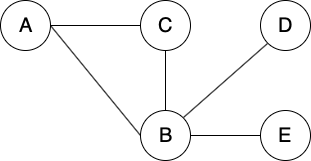
\includegraphics[width=\linewidth]{images/undirected_unweighted_graph.png}
     \caption{Undirected unweighted graph}
  \end{subfigure}
  \hfill
  \begin{subfigure}[b]{0.18\linewidth}
    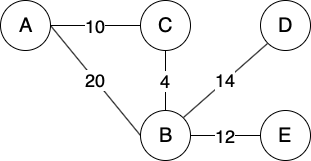
\includegraphics[width=\linewidth]{images/undirected_weighted_graph.png}
    \caption{Undirected weighted graph}
  \end{subfigure}
  \hfill
  \begin{subfigure}[b]{0.18\linewidth}
    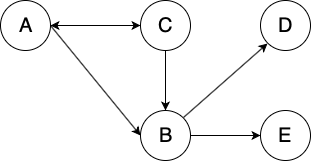
\includegraphics[width=\linewidth]{images/directed_unweighted_graph.png}
    \caption{Directed unweighted graph}
  \end{subfigure}
  \hfill
  \begin{subfigure}[b]{0.18\linewidth}
    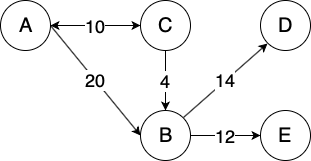
\includegraphics[width=\linewidth]{images/directed_weighted_graph.png}
    \caption{Directed weighted graph}
  \end{subfigure}
  \caption{Graph examples. The nodes are represented with a circle, and the identifier is the letter inside them. The edges are represented by lines or arrows, and the values from them represent weight values}
  \label{fig:graphs}
\end{figure}

A grid (See Figure \ref{fig:grids}) is a two-dimensional table that allows movement to nearby cells. This data structure can be easily translated to an undirected unweighted graph where grid cells represent nodes and neighbours represent undirected edges. The neighbours are defined in terms of the grid connectivity type which can be 4-point connectivity (up, down, left, right) or 8-point connectivity (all 4-point connectivity neighbours, principal diagonal and secondary diagonal) \cite{choset2005principles}. We are going to assume 8-point connectivity for all grids unless explicitly stated.

\begin{figure}[h!]
  \centering
  \begin{subfigure}[b]{0.18\linewidth}
    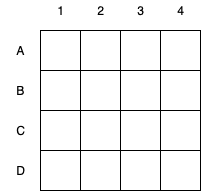
\includegraphics[width=\linewidth]{images/4x4_grid.png}
     \caption{4$\times$4 normal grid\newline\newline}
  \end{subfigure}
  \hfill
  \begin{subfigure}[b]{0.18\linewidth}
    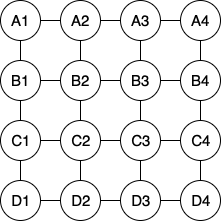
\includegraphics[width=\linewidth]{images/4_way_graph.png}
    \caption{4-point connectivity graph representation}
  \end{subfigure}
  \hfill
  \begin{subfigure}[b]{0.18\linewidth}
    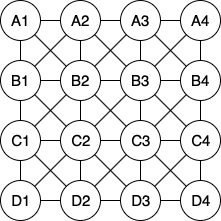
\includegraphics[width=\linewidth]{images/8_way_graph.png}
    \caption{8-point connectivity graph representation}
  \end{subfigure}
  \caption{4x4 grid example with associated 4-point and 8-point connectivity graphs. In 4-point connectivity, the neighbours are up, down, left and right. In 8-point connectivity, the neighbours are all 4-point connectivity neighbours, the principal diagonal and the secondary diagonal. The numbers at the top and left of the grid represent coordinates}
  \label{fig:grids}
\end{figure}

A tree (See Figure \ref{fig:trees}) is a directed graph with a root (i.e. a node that has no incoming edges) where each node has directed edges to their children. A particular property of the tree is that it contains no cycles. This data structure is essential as most algorithms have to walk the graph in some way (depth-first search, breadth-first search) in order to discover a possible path. Depth-first search (DFS) \cite{Cormen:2009:IAT:1614191} is a graph walking method that can be implemented using a stack (Last In First Out (LIFO) data structure) or recursion (stack is preferred, due to the recursion depth constraint that most programming languages incorporate). DFS starts by “expanding” the root (i.e. visit the node and push the node’s children onto the stack) and then iteratively expands the latest node from the stack. Thus, we initially visit the first children of the node we expand and then visit its children recursively before continuing with the second child. Breadth-first search (BFS) \cite{Cormen:2009:IAT:1614191} is another graph walking method that uses a queue (First In First Out FIFO data structure). BFS starts by expanding the root and then it repeats the process iteratively for the children. Thus we first visit \textbf{all} of the children of the node we expand and then we continue to expand each child. When BFS has to expand a node, it chooses the one in the front of the queue, and then it puts \textbf{all} of the children at the end of the queue. The result of both methods is a tree \cite{choset2005principles}.

\begin{figure}[h!]
  \centering
  \begin{subfigure}[b]{0.18\linewidth}
    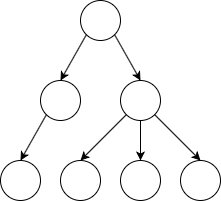
\includegraphics[width=\linewidth]{images/tree_example.png}
     \caption{A tree}
  \end{subfigure}
  \hfill
  \begin{subfigure}[b]{0.18\linewidth}
    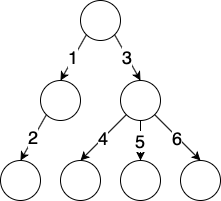
\includegraphics[width=\linewidth]{images/dfs.png}
    \caption{DFS walk}
  \end{subfigure}
  \hfill
  \begin{subfigure}[b]{0.18\linewidth}
    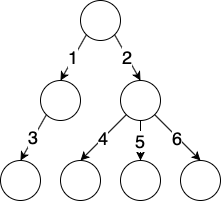
\includegraphics[width=\linewidth]{images/bfs.png}
    \caption{BFS walk}
  \end{subfigure}
  \caption{An example of a tree along with a DFS and BFS walk. The numbers indicate the order of expansions}
  \label{fig:trees}
\end{figure}

The worst case time complexity of DFS is $\mathcal{O}(b^d)$ and the worst case space complexity is $\mathcal{O}(b \cdot d)$ if a stack is used and $\mathcal{O}(d)$ if recursion is used, where $b$ is the branching factor (the average number of a node's children) and $d$ is the visiting depth. Time complexity is trivial as at each step we run a new search for all the node children $b$, and we do this $d$ times. If we use a stack, for each node, we push all children onto the stack. We do this $d$ times, and each node has $b$ children. Therefore the space complexity is $\mathcal{O}(b \cdot d)$. When using recursion, the space complexity is lower as it is defined in terms of the recursion depth (we do not use all children at once at each recursion step). However, we still prefer to use the stack in practice, due to the programming language limitations \cite{Cormen:2009:IAT:1614191}.

The worst case time and space complexity of BFS is $\mathcal{O}(b^d)$. The time complexity follows the same reasoning as DFS. Space complexity is given by the number of nodes in the queue at one time which is equal to the number of the nodes on each layer of the tree which is $\mathcal{O}(b^d)$ as each layer node count grows exponentially \cite{Cormen:2009:IAT:1614191}.

When talking about complexities we have opted for the $b$ (branching factor) and $d$ (depth) notation instead of the $|E|$ (number of edges) and $|V|$ (number of vertices/nodes) (e.g. DFS space complexity is the same as BFS space complexity $\mathcal{O}(|V|)$). We are going to discuss algorithms which attempt to prune the search space, and we can infer more information from the first notation rather than the second one \cite{Cormen:2009:IAT:1614191}.

In practice, we prefer to use BFS when dealing with problems that attempt to find an optimal solution (due to the visiting pattern) and DFS when we want to visit the whole tree without caring about the visiting pattern or when we have memory constraints.

\subsection{Wave-front Planner} \label{sec: wave-front}
The Wave-front Planner algorithm \cite{choset2005principles, luo2014effective} (See Figure \ref{fig:wave_front_planner}) is one of the simplest solutions to the pathfinding problem. The algorithm can only run on grids (two dimensional or higher). The main idea is to have a separate grid with initial values of 0 then "propagate" a wave from the goal position to the agent position. Thus, we essentially create a potential function on the grid. 

The wave is propagated by applying BFS to the separate grid from the goal position and then labelling the nodes on the same level of the tree with the level number. Thus, we first visit all the (valid) neighbours of the goal and mark the positions on the new grid with a 2 (as the goal position is marked with 1). Then we repeat the process for the nodes labelled with a 2 by expanding them and marking their \textbf{not visited} neighbours with a 3. The process is repeated until we hit the agent position. After that, we apply gradient descent from the agent position to the goal position. We start from the agent marked with number $x$ and then search its neighbours for a node marked with $x-1$. If there are multiple choices we can choose a random number as the invariant of the algorithm states that, given any node, the distance between itself and the agent is the absolute difference between their grid values (See Algorithm \ref{alg: wave_front_planner}).

% figures align
\vspace{-0.5cm}
$$dist(n) = abs(grid(G) - grid(n))$$
\vspace{-0.5cm}

We can easily prove that the algorithm finds the optimal solution in terms of minimum distance as we have used BFS to expand the nodes. If we would have used DFS instead, we could have still found a solution, but it would not necessarily be optimal due to the visiting pattern in DFS. The path might not be optimal in environments where the edge transition cost is not equal in all directions (e.g. moving on the diagonal ($\sqrt{2}$) is more expensive than moving vertically or horizontally (1) based on the Euclidean distance).

The worst case time and space complexity are given by the visiting method (BFS in our case) which is $\mathcal{O}(b^d)$, where $b$ is the branching factor, and $d$ is the depth of the solution (\textit{Get-Backtrace} is $\mathcal{O}(d)$).

One of the major drawbacks to this approach is that the optimal path is dangerously close to the obstacles (as only the attraction function is used) and in the real world, it might lead to collisions. It is also computationally expensive as the planner's search space is quite large since it does not apply any pruning. Moreover, the time and space complexity increase exponentially with the dimension of the environment. In a 2D grid with 8-point connectivity $b$ is 8, but in a 3D grid world $b$ is $3 \times 9 - 1 = 26$ (we subtract the (0, 0, 0) direction), where $b$ is the branching factor. A nice way to visualise the increase of $b$ is to count the number of combinations on each direction. Each coordinate has 3 configurations (1, 0, -1) and the number of combinations is given by $3^D$, where $D$ is the dimension. Therefore, $b = 3^D - 1$ (we have to subtract the (0, 0, ..., 0) configuration as it is not a valid neighbour). Therefore, time and space complexity becomes $\mathcal{O}((3^D)^d)$. However, because we are working with real-world robots, we can only consider 2D and 3D environments (2D for ground robot, 3D for drones and flying robots).

% A possible memory optimisation is to use the same input grid if the grid entities are labelled with a number (0 clear, 1 wall, -1 agent, 2 goal). However one requirement is that the goal has to be identified with a number higher then all other available entities.

\begin{figure}[]
  \centering
  \begin{subfigure}[b]{0.2\linewidth}
    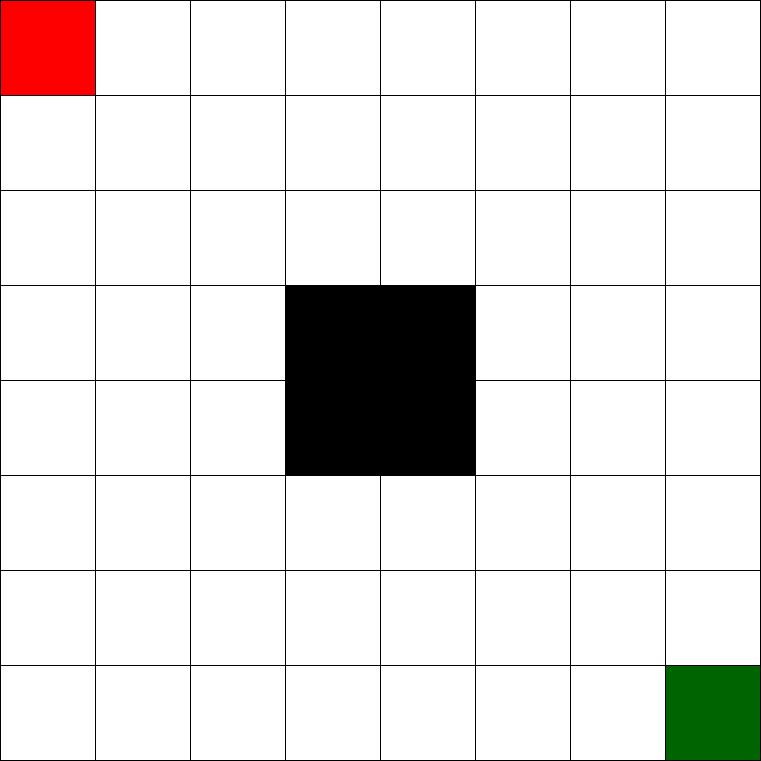
\includegraphics[width=\linewidth]{images/simple_grid.png}
     \caption{Starting 8x8 grid}
  \end{subfigure}
  \hfill
  \begin{subfigure}[b]{0.2\linewidth}
    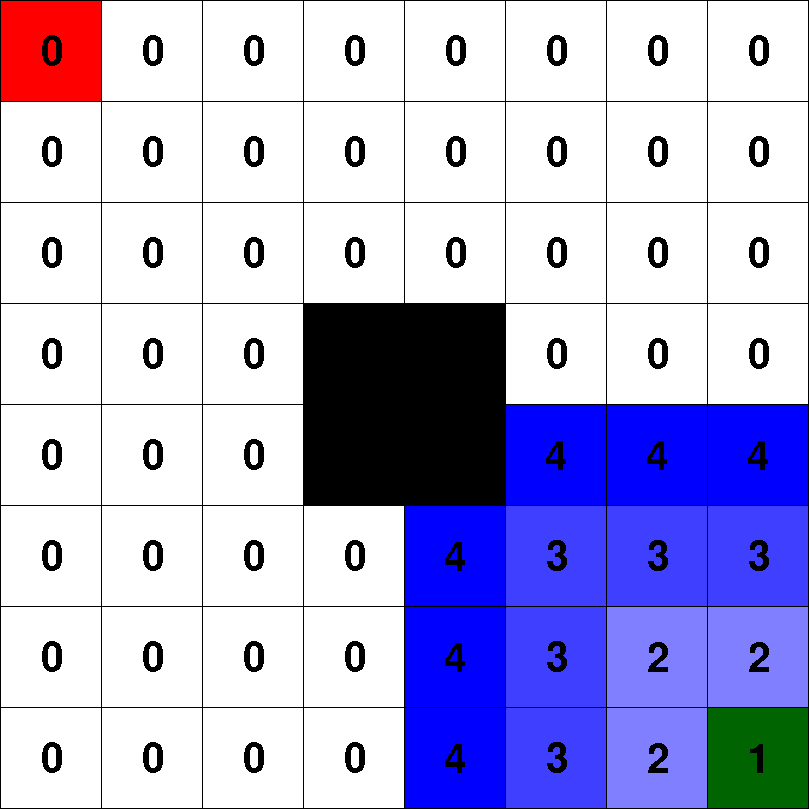
\includegraphics[width=\linewidth]{images/wave_front_planner_1.png}
     \caption{Iteration 1}
  \end{subfigure}
  \hfill
  \begin{subfigure}[b]{0.2\linewidth}
    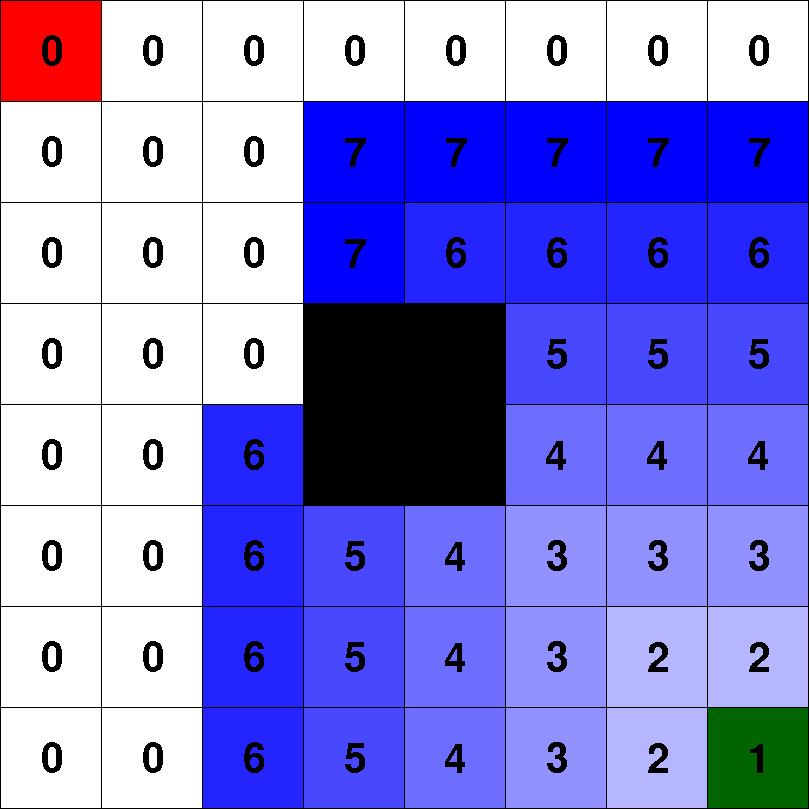
\includegraphics[width=\linewidth]{images/wave_front_planner_2.png}
    \caption{Iteration 2}
  \end{subfigure}
  \hfill
  \begin{subfigure}[b]{0.2\linewidth}
    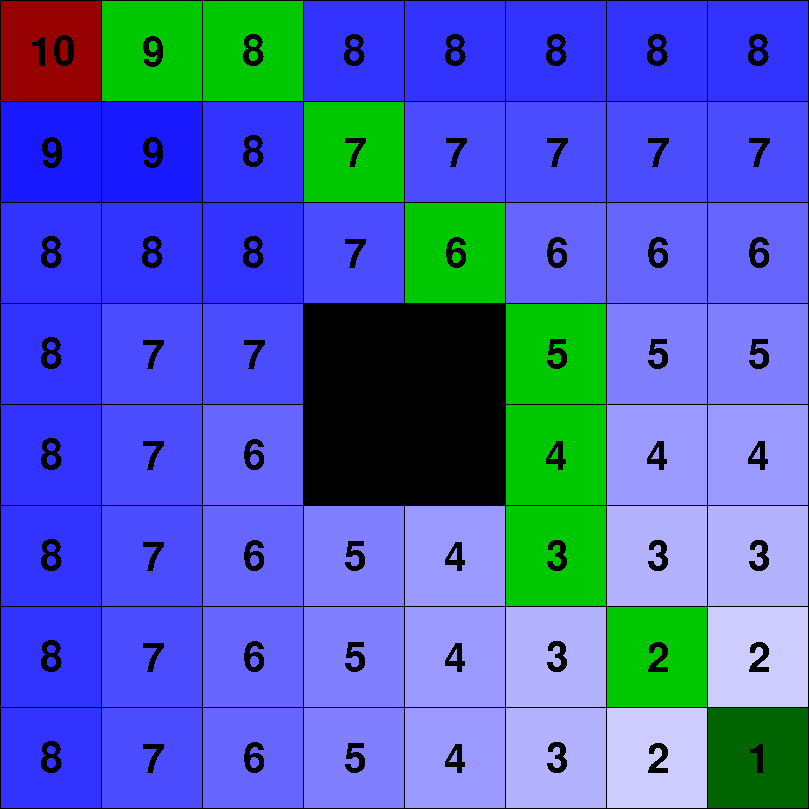
\includegraphics[width=\linewidth]{images/wave_front_planner_3.png}
    \caption{Final trace}
  \end{subfigure}
  \caption{Wave-front Planner algorithm run on an 8x8 grid (4 iteration points shown: start, 1, 2, final trace). The red square represents the agent start position, the dark green square represents the goal position, black squares represent obstacles, white squares represent the clear path, light green squares represent the final path chosen by the algorithm. The numbers in each grid cell represent the gradient map and the white (min) - dark blue (max) gradient colour is another representation of the gradient map}
  \label{fig:wave_front_planner}
\end{figure}

\begin{algorithm}[h!]
\caption{Wave-Front Planner}
\label{alg: wave_front_planner}
\begin{algorithmic}[1]

\Procedure{Get-Backtrace}{$step\_grid$, $M\colon(A, Os, G)$}
    \State $trace \gets [A]$
    % \State
    \While {$current$ is not $A$}
        \State $current \gets \forall n \in Neighbours(current). step\_grid[n] = step\_grid[current] - 1$
        \State add $current$ to $trace$
    \EndWhile
    % \State
    \State \Return $trace$
\EndProcedure
\\
    
\Procedure{Wave-Front-Planner}{$M\colon(A, Os, G)$}
    \State Initialize queue $q$ with (1, $G$)
    \State Initialize $step\_grid$ as array with same size as map
    \State $visited \gets \{\}$
    \State
    \Repeat
        \State ($current\_count$, $current\_node$) $\gets$ pop front $q$
        \State add $current\_node$ to $visited$
        \State $step\_grid[current\_node]$ $\gets$ $current\_count$
        \State
        \If {$current\_node$ is $A$}
            \State follow $\textit{Get-Backtrace}(step\_grid, M)$
            \State \Return 
        \EndIf
        \State
        \For {\textbf{each} $neighbour$ in $Neighbours(current\_node)$}
            \If {$neighbour$ is not in $visited$}
                \State append ($current\_count$ + 1, $neighbour$) to $q$
            \EndIf
        \EndFor
    \Until $q$ is empty
    \State
    \State goal was not found
\EndProcedure
\end{algorithmic}
\end{algorithm}

\subsection{A*} \label{sec:a_star}
The A* algorithm \cite{choset2005principles, duchovn2014path, zhang2014multiple, 5937169} (See figures \ref{fig:a_star}, \ref{fig:a_star_expansion}) is mostly designed to run on weighted graphs, but can be adapted to run on grids as well if we convert the grid to a graph with weights based on the Euclidean distance (1 for vertical/horizontal movement and $\sqrt{2}$ for diagonal movement).

The difference between A* and Wave-front Planner is that A* aims to prune the search space by using a heuristic function $h$ which is usually the Euclidean distance (8-point connectivity) or the Manhattan distance (4-point connectivity) (See Figure \ref{fig:distances}).

\begin{figure}[h!]
  \centering
  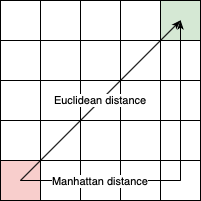
\includegraphics[scale=0.5]{images/distances.png}
  \caption{Euclidean and Manhattan distances. Red square is agent and green square is goal}
  \label{fig:distances}
\end{figure}

It is implemented using a priority queue in which the priorities are a function $f(n) = g(n) + h(n)$, where $h$ is the heuristic function mentioned above and $g$ is a function which represents the total actual distance travelled from the agent to the node $n$. The cost function $c(x, y)$ returns the graph weight cost from node $x$ to node $y$ ($x$ and $y$ have to be connected). The algorithm starts with the agent node in the priority queue. Then, the element with the highest priority (i.e. lowest $f(n)$) is picked and expanded, and its children are inserted into the priority queue. Each child will have a parent $p$, which will help us trace back the path at the end. When we expand a child we set $p(child) = n$. If a path is found, we update the goal parent. We stop the process only when the priority queue is empty or when the next priority is less than or equal to the optimal distance found. All expanded nodes are marked as seen, so we do not have to revisit them. When we expand a node, if any of its children are already in the queue we add them again if the path through the current node gives a higher priority ($g(n) < g(child)$) and update the child's parent ($p(child) = n, g(child) = g(n) + c(n, child)$). It does not matter if we add the children again to the queue as we know that $f_{cur}(child) < f_{old}(child)$ so we will visit the higher priority option first. When we stop, we compute the trace by recursively looking at the next parent from the goal until we find the agent (See Figure \ref{fig:a_star_expansion}, Algorithm \ref{alg: a_star}).

A* finds the shortest path, if and only if, the heuristic function is optimistic. An optimistic heuristic function is always less than or equal to the shortest distance.

The worst case time and space complexity of A* is $\mathcal{O}(b^d)$, where $b$ is the branching factor, and $d$ is the depth of the solution because the underlying algorithm structure is similar to BFS (\textit{Get-Backtrace} is $\mathcal{O}(d)$). However, by using a good heuristic function, the time and space complexity becomes $\mathcal{O}(\hat{b}^d)$ where $\hat{b}$ is the reduced branching factor (i.e. A* prunes the search).

% \todo{Cite wikipedia and stackoverflow??}
% https://en.wikipedia.org/wiki/A*_search_algorithm
% https://cs.stackexchange.com/questions/56176/a-graph-search-time-complexity

The significant advantage of A* is that the search space is pruned quite a lot, but it still shares the same issue as the other graph search planners: the search space grows exponentially with the grid dimension.

One of the major drawbacks is that it is not trivial to find a proper heuristic function for some environments (e.g. maps that do not define a metric space such as networks). In general, the Euclidean distance or the Manhattan distance are good choices for the heuristic function. Lastly, A* is an offline method (the internal state of the algorithm cannot be externally modified) meaning that external updates to the map are forbidden. Therefore, offline algorithms such as A* do not support dynamic and partial knowledge environments.

\pagebreak

\begin{figure}[h!]
  \centering
  \begin{subfigure}[b]{0.2\linewidth}
    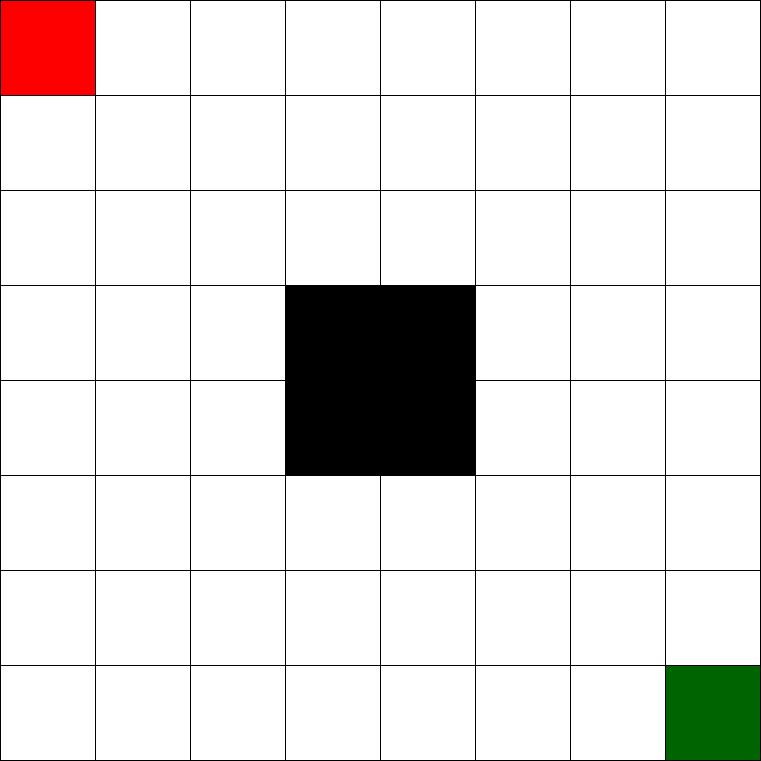
\includegraphics[width=\linewidth]{images/simple_grid.png}
     \caption{Starting 8x8 grid}
  \end{subfigure}
  \hfill
  \begin{subfigure}[b]{0.2\linewidth}
    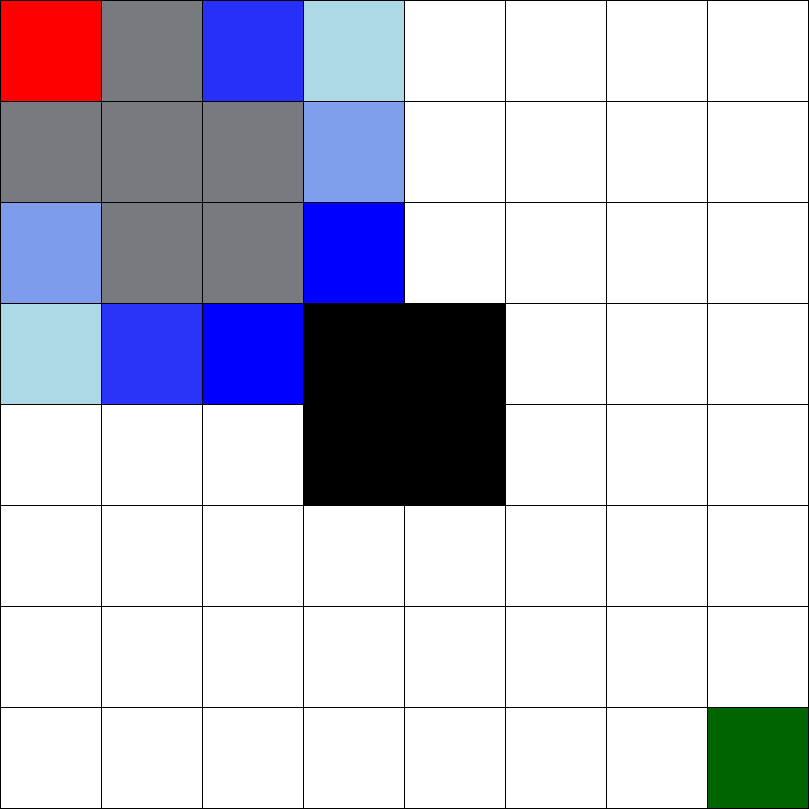
\includegraphics[width=\linewidth]{images/a_star_1.png}
     \caption{Iteration 1}
  \end{subfigure}
  \hfill
  \begin{subfigure}[b]{0.2\linewidth}
    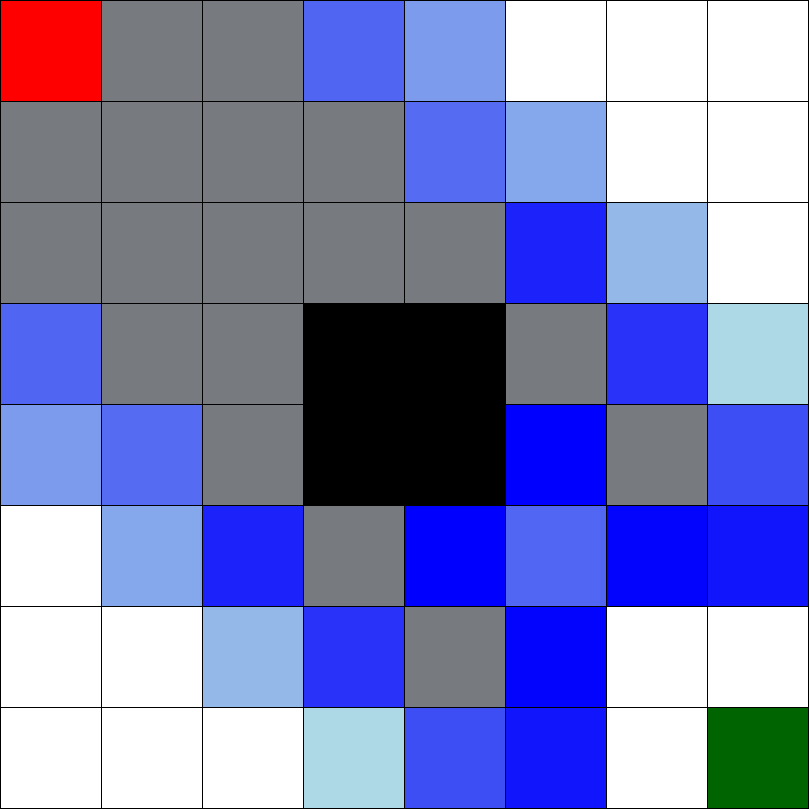
\includegraphics[width=\linewidth]{images/a_star_2.png}
    \caption{Iteration 2}
  \end{subfigure}
  \hfill
  \begin{subfigure}[b]{0.2\linewidth}
    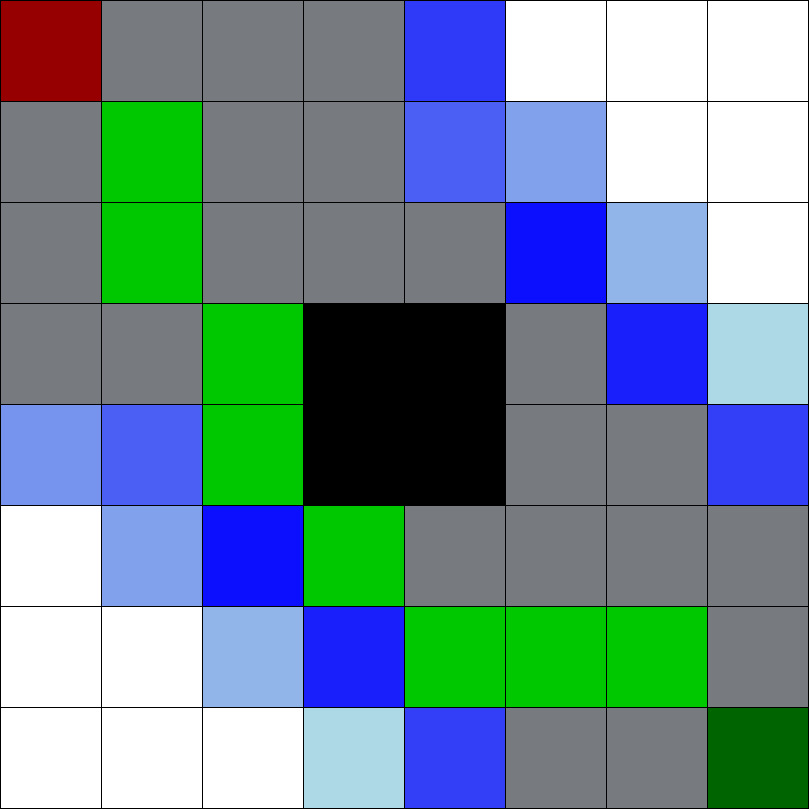
\includegraphics[width=\linewidth]{images/a_star_3.png}
    \caption{Final trace}
  \end{subfigure}
  \caption{A* algorithm run on an 8$\times$8 grid (4 iteration points shown: start, 1, 2, final trace). The red square represents agent start position, the dark green square represents the goal position, black squares represent obstacles, white squares represent the clear path, light green squares represent the final path chosen by the algorithm. The dark grey squares represent the visited set, and the blue squares represent the priority queue (the darker the blue, the higher the priority)}
  \label{fig:a_star}
\end{figure}

\begin{figure}[h!]
  \centering
  \begin{subfigure}[b]{0.2\linewidth}
    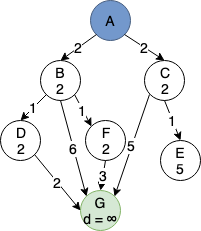
\includegraphics[width=\linewidth]{images/a_star_expansion1.png}
     \caption{Iteration 1}
  \end{subfigure}
  \hfill
  \begin{subfigure}[b]{0.2\linewidth}
    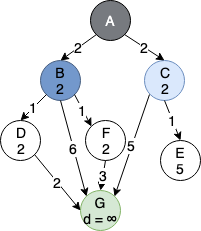
\includegraphics[width=\linewidth]{images/a_star_expansion2.png}
     \caption{Iteration 2}
  \end{subfigure}
  \hfill
  \begin{subfigure}[b]{0.2\linewidth}
    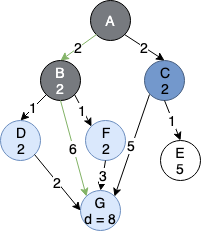
\includegraphics[width=\linewidth]{images/a_star_expansion3.png}
    \caption{Iteration 3}
  \end{subfigure}
  \newline
  \begin{subfigure}[b]{0.2\linewidth}
    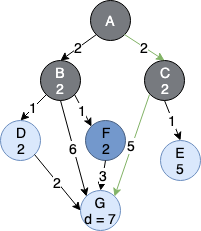
\includegraphics[width=\linewidth]{images/a_star_expansion4.png}
     \caption{Iteration 4}
  \end{subfigure}
  \hfill
  \begin{subfigure}[b]{0.2\linewidth}
    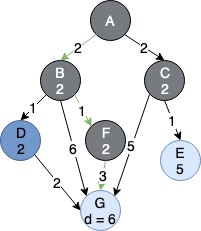
\includegraphics[width=\linewidth]{images/a_star_expansion5.png}
     \caption{Iteration 5}
  \end{subfigure}
  \hfill
  \begin{subfigure}[b]{0.2\linewidth}
    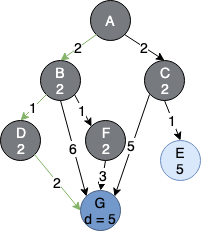
\includegraphics[width=\linewidth]{images/a_star_expansion6.png}
    \caption{Iteration 6}
  \end{subfigure}
  \hfill
  \begin{subfigure}[b]{0.2\linewidth}
    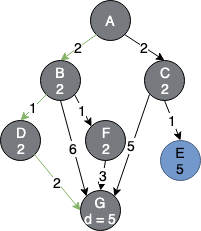
\includegraphics[width=\linewidth]{images/a_star_expansion7.png}
    \caption{Iteration 7}
  \end{subfigure}
  \caption{A* algorithm run on a directed weighted graph. Nodes are labelled with a letter that represents its name (A and G are special nodes agent and goal respectively) and the optimistic heuristic value. Edges have an associated value with them, which represents the actual distance between them. The green node is the goal, dark grey nodes are visited nodes, light blue and dark blue nodes are belonging to the priority queue, dark blue nodes are the next nodes to be expanded, green arrow trace is the optimal solution so far and $d = x$ label is optimal total distance so far}
  \label{fig:a_star_expansion}
\end{figure}

\pagebreak

\begin{algorithm}[h!]
\caption{A*}
\label{alg: a_star}
\begin{algorithmic}[1]

\Procedure{Get-Backtrace}{$p$, $M\colon(A, Os, G)$}
    \State $current \gets$ $G$
    \State $trace \gets [current]$
    \State
    \While {$current$ is not $A$}
        \State $current \gets p[$current$]$
        \State add $current$ to $trace$
    \EndWhile
    \State
    \State \Return reversed $trace$
\EndProcedure
\\

\Procedure{A*}{$M\colon(A, Os, G)$}
    \State Initialize priority queue $pq$ with ($f(A)$, $A$)
    \State $visited \gets \{\}$
    \State $p \gets \{\colon\}$
    \Repeat
        \State $current\_node$ $\gets$ best $n_{best}$ from $pq$ where $\forall n.f(n_{best}) \leq f(n)$
        \State add $current\_node$ to $visited$
        \State
        \If {$current\_node$ is $G$}
            \State follow $\textit{Get-Backtrace}(p, M)$
            \State \Return
        \EndIf
        \State
        \For {\textbf{each} $neighbour$ in $Neighbours(current\_node)$}
            \If {$neighbour$ is not in $visited$ \textbf{or} $g(current\_node) + c(current\_node, neighbour) < g(neighbour)$}
                \State $g(neighbour) \gets g(current\_node) + c(current\_node, neighbour)$
                \State add $neighbour$ to $pq$
                \State update $p[neighbour]$ to $current\_node$
            \EndIf
        \EndFor
    \Until $visited$ is empty
    \State
    \State goal was not found
\EndProcedure
\end{algorithmic}
\end{algorithm}

\subsection{Dijkstra} \label{sec: dijkstra}
The Dijkstra algorithm \cite{choset2005principles, zhang2014multiple} (See Figures \ref{fig:dijkstra}, \ref{fig:dijkstra_expansion}) is a variation of the A* algorithm where we omit the heuristic function ($f(n) = g(n)$). Therefore the algorithm becomes greedy, meaning that we expand the node with lowest distance from the agent position. (See Figure \ref{fig:dijkstra_expansion}). The algorithm is identical to A* (See Algorithm \ref{alg: a_star}), but with $f(n) = g(n)$. Thus, the space and time complexity is the same as A* $(\mathcal{O}(\hat{b}^d))$, but $\hat{b}$ is usually not as efficient as A*.

The major difference between A* and Dijkstra is that, because it is a greedy algorithm, once we expand the goal node, we find the final solution. The solution is optimal in terms of minimal distance because after we expand a node, its distance will not be modified in the future (the invariant holds for all nodes, not only for the goal). 

The drawback of using this method against A* is that it usually explores more than A* and thus the memory gets quite high.

\pagebreak

\begin{figure}[h!]
  \centering
  \begin{subfigure}[b]{0.2\linewidth}
    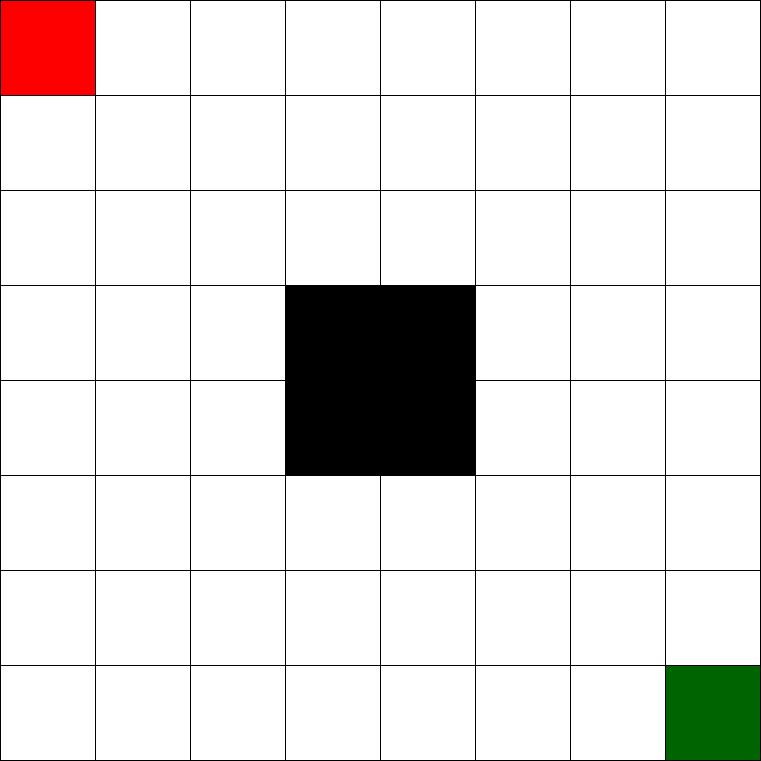
\includegraphics[width=\linewidth]{images/simple_grid.png}
     \caption{Starting 8x8 grid}
  \end{subfigure}
  \hfill
  \begin{subfigure}[b]{0.2\linewidth}
    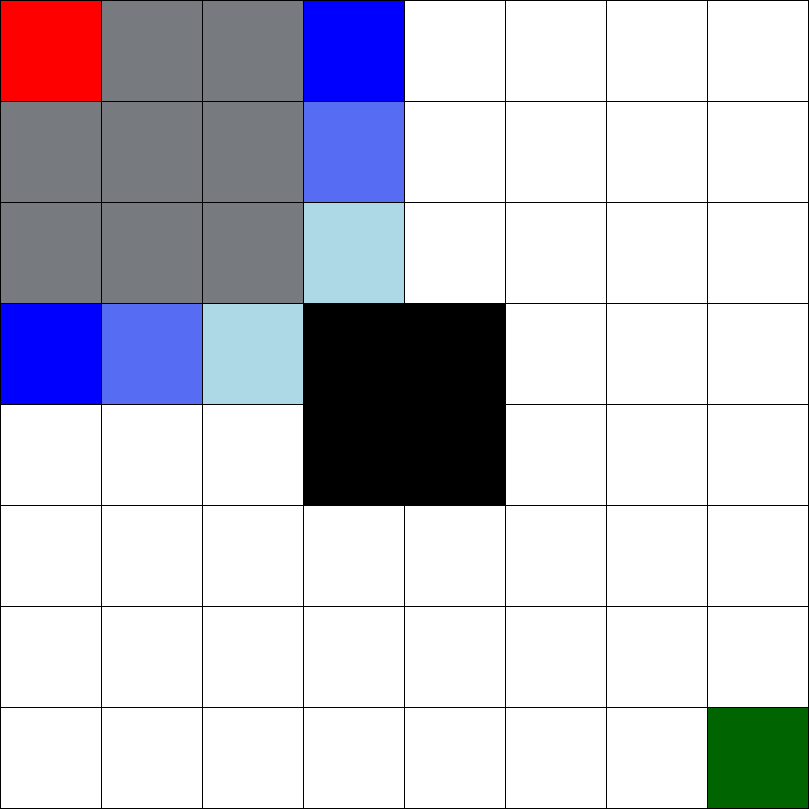
\includegraphics[width=\linewidth]{images/dijkstra1.png}
     \caption{Iteration 1}
  \end{subfigure}
  \hfill
  \begin{subfigure}[b]{0.2\linewidth}
    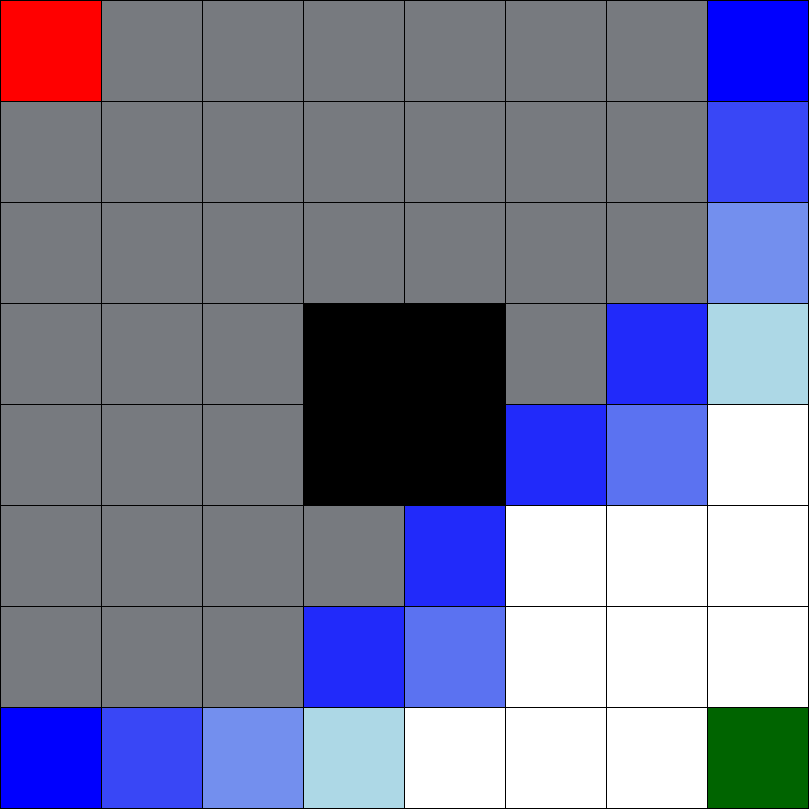
\includegraphics[width=\linewidth]{images/dijkstra2.png}
    \caption{Iteration 2}
  \end{subfigure}
  \hfill
  \begin{subfigure}[b]{0.2\linewidth}
    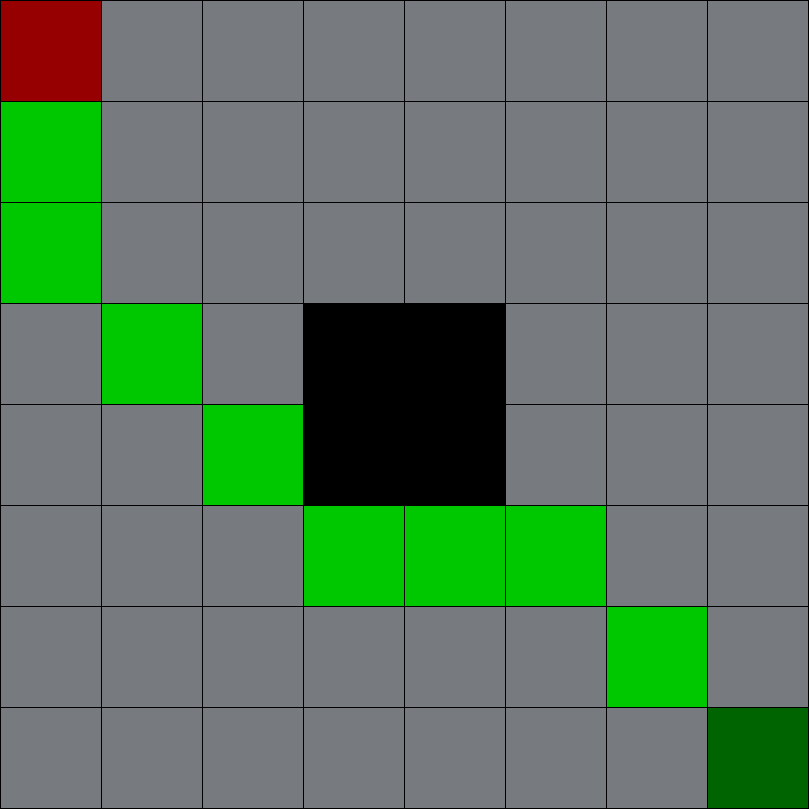
\includegraphics[width=\linewidth]{images/dijkstra3.png}
    \caption{Final trace}
  \end{subfigure}
  \caption{Dijkstra algorithm run on an 8$\times$8 grid (4 iteration points shown: start, 1, 2, final trace). The red square represents the agent start position, the dark green square represents the goal position, black squares represent obstacles, white squares represent the clear path, light green squares represent the final path chosen by the algorithm. The dark grey squares represent the visited set, and the blue squares represent the priority queue (the darker the blue, the higher the priority)}
  \label{fig:dijkstra}
\end{figure}

\begin{figure}[h!]
  \centering
  \begin{subfigure}[b]{0.2\linewidth}
    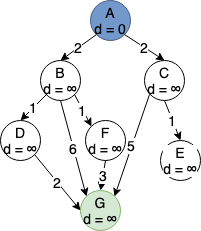
\includegraphics[width=\linewidth]{images/dijkstra_expansion1.png}
     \caption{Iteration 1}
  \end{subfigure}
  \hfill
  \begin{subfigure}[b]{0.2\linewidth}
    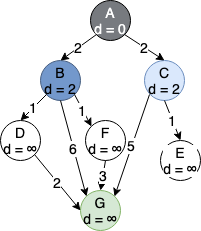
\includegraphics[width=\linewidth]{images/dijkstra_expansion2.png}
     \caption{Iteration 2}
  \end{subfigure}
  \hfill
  \begin{subfigure}[b]{0.2\linewidth}
    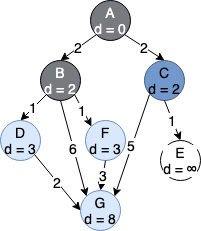
\includegraphics[width=\linewidth]{images/dijkstra_expansion3.png}
    \caption{Iteration 3}
  \end{subfigure}
  \hfill
  \begin{subfigure}[b]{0.2\linewidth}
    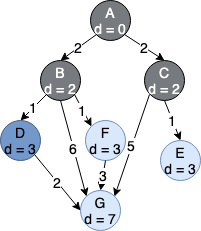
\includegraphics[width=\linewidth]{images/dijkstra_expansion4.png}
     \caption{Iteration 4}
  \end{subfigure}
  \newline
  \begin{subfigure}[b]{0.2\linewidth}
    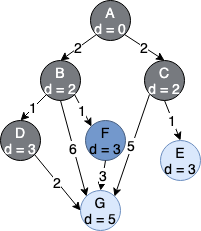
\includegraphics[width=\linewidth]{images/dijkstra_expansion5.png}
     \caption{Iteration 5}
  \end{subfigure}
  \hfill
  \begin{subfigure}[b]{0.2\linewidth}
    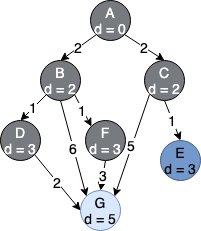
\includegraphics[width=\linewidth]{images/dijkstra_expansion6.png}
    \caption{Iteration 6}
  \end{subfigure}
  \hfill
  \begin{subfigure}[b]{0.2\linewidth}
    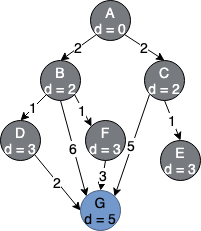
\includegraphics[width=\linewidth]{images/dijkstra_expansion7.png}
     \caption{Iteration 7}
  \end{subfigure}
  \hfill
  \begin{subfigure}[b]{0.2\linewidth}
    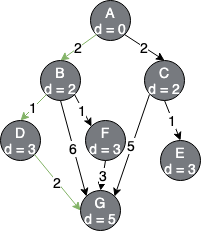
\includegraphics[width=\linewidth]{images/dijkstra_expansion8.png}
    \caption{Iteration 8}
  \end{subfigure}
  \hfill
  \caption{Dijkstra algorithm run on a directed weighted graph. Nodes are labelled with a letter identifier (A and G are special nodes agent and goal respectively) and the current distance. The distance is final when the node is marked as visited. Edges have an associated value with them, which represents edge weight. The green node is the goal, dark grey nodes are visited nodes, light blue and dark blue nodes are belonging to the priority queue, dark blue nodes are the next nodes to be expanded, green arrow trace is the optimal solution}
  \label{fig:dijkstra_expansion}
\end{figure}

\pagebreak

\subsection{Bug Algorithms}
The bug algorithms \cite{choset2005principles, rajko2001pursuit} are one of the earliest and simplest sensor-based solutions for the pathfinding problem, and we will cover two implementations: Bug1 and Bug2. There exist other algorithms which are more advanced such as Tangent Bug described in \cite{choset2005principles, rajko2001pursuit, kamon1998tangentbug}, but we will not cover them as it exceeds the scope of our report.

The idea behind bug algorithms is based on the instinctual behaviour of a bug moving directly towards a destination (goal) and turning around encountered obstacles. The algorithms have two phases: straight line movement (phase 1) and object boundary following (phase 2). We will assume that the agent has a contact sensor that detects if the agent is in the proximity of the boundary of an obstacle.

%We will cover the boundary following algorithm at the end of this section.

The bug algorithms are trivial to implement, not computationally expensive, and it has been shown that their success is guaranteed, meaning that they can find a path to the goal if one exists. However, they do not find the optimal path.

\subsubsection{Bug1} \label{sec: bug1}

First, we label the direction from the agent position to the goal position with $dir_{AG} = \frac{d(A, G)
}{\norm{d(A, G)}} = \frac{(G - A)} {\norm{G - A}}$. In the first phase, the algorithm follows $dir_{A, G}$ until an obstacle is detected and we mark this position as $P_{i}$. Afterwards, it proceeds with the second phase by doing a complete loop around the obstacle while registering the closest distance on the boundary to the goal (find $\hat{Ob} = \argmin{Ob}{d_{Ob, G}}, Ob \in Boundary(O)$) until we reach $P_{i}$. After that, we follow the boundary again until we reach $\hat{Ob}$ and return to the first phase. We repeat this process until the goal is found. If the agent were to move, but it can't from $\hat{Ob}$, then we conclude the algorithm as the goal is unreachable (See Figure \ref{fig:Bug1}, See Algorithm \ref{alg: bug1}) \cite{lumelsky1986dynamic}.

As it is quite hard to estimate the worst case time complexity, we are going to express it as the number of steps upper bound ($\mathcal{O}(upper_{Bug1})$). The upper bound on the number of steps is given by the total distance from the agent to the goal $d(A, G)$, in the case of no obstacles, plus the worst case traversed boundary length for all obstacles $1.5 \sum_{o \in O} length(Boundary(o))$. The space complexity is $\mathcal{O}(1)$ (not counting recursion steps as it can be collapsed in a while loop).

$$upper_{Bug1} = d(A, G) + 1.5 \sum_{o \in O} length(Boundary(o))$$

\begin{figure}[h!]
  \centering
  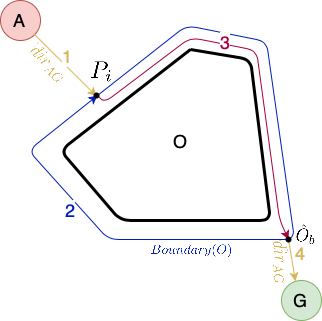
\includegraphics[scale=0.4]{images/Bug1.png}
  \caption{Bug1: Arrows represent the movement direction and numbers represent the traversal order. Yellow arrows represent the first phase. Blue and red arrows represent the second phase}
  \label{fig:Bug1}
\end{figure}

\begin{algorithm}
\caption{Bug1}
\label{alg: bug1}
\begin{algorithmic}[1]
\Procedure{Bug1}{$M\colon(A, Os, G)$}
    \State $\textit{Phase1}(M)$
\EndProcedure
\\
\Procedure{Phase1}{$M\colon(A, Os, G)$}
    \State move agent towards goal along $dir_{A, G}$ until hits $P_i$ or $G$
    \If {$G$ was reached}
        \State \Return
    \EndIf
    \State $\textit{Phase2}(M, P_i)$
\EndProcedure
\\
\Procedure{Phase2}{$M\colon(A, Os, G)$, $P_i$}
    \State find obstacle $O$ with hit point $P_i$ from $Os$
    \State do a full loop around $Boundary(O)$ while computing $\hat{O}b$
    \State follow $Boundary(O)$ until $\hat{O}b$ is reached
    \State
    \If {can't move from $\hat{Ob}$ to $G$}
        \State goal can't be reached
        \State \Return
    \EndIf
    \State
    \State $\textit{Phase1}(M)$
\EndProcedure
\end{algorithmic}
\end{algorithm}

\subsubsection{Bug2} \label{sec: bug2}
The first stage is identical to the one in Bug1, but the second stage follows a greedy approach. Instead of making a full obstacle loop in the second stage, we try to find the point $P \in Boundary(O)$ which belongs to the line segment determined by the original starting agent position and the goal position $P \in LS_{A_{initial}, G}$. $P$ should also be chosen in such a way that it is closer than the original point of contact with the obstacle $P_i$. If $P = P_i$ then the goal can't be reached (See Figure \ref{fig:Bug2}, See Algorithm \ref{alg: bug2}) \cite{lumelsky1986dynamic}.

However, this does not imply that Bug2 outperforms Bug1 in all cases. The time complexity (given as the upper bound) for Bug2 is determined by the total distance from the agent to the goal $d(A, G)$, in the case of no obstacles, plus the worst case traversed boundary length for all obstacles $0.5 \sum_{o \in O} n_{o} \cdot length(Boundary(o))$. The issue here is that, because we follow a greedy approach, we might reencounter the same obstacle, thus $n_{o}$ represents how many times we have encountered obstacle $o$. Therefore, Bug1 might yield better performance in cases where the environment contains complex obstacles. The space complexity is still $\mathcal{O}(1)$.

$$upper_{Bug2} = d(A, G) + 0.5 \sum_{o \in O} n_{o} \cdot length(Boundary(o))$$

\begin{figure}[h!]
  \centering
  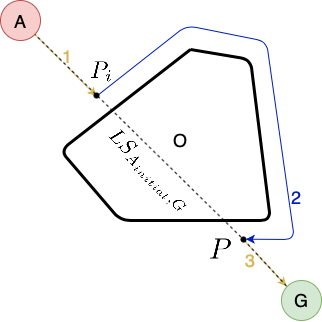
\includegraphics[scale=0.4]{images/Bug2.png}
  
  \caption{Bug2: Arrows represent the movement direction and numbers represent the traversal order. Yellow arrows represent the first phase. Blue arrows represent the second phase}
  \label{fig:Bug2}
\end{figure}

\begin{algorithm}[h]
\caption{Bug2}
\label{alg: bug2}
\begin{algorithmic}[1]
\Procedure{Bug2}{$M\colon(A, Os, G)$}
    \State $\textit{Phase1}()$
\EndProcedure
\\
\Procedure{Phase1}{$M\colon(A, Os, G)$}
    \State move agent towards goal along $LS_{A_{initial}, G}$ until hits $P_i$ or $G$
    \If {$G$ was reached}
        \State \Return
    \EndIf
    \State $\textit{Phase2}(M, P_i)$
\EndProcedure
\\
\Procedure{Phase2}{$M\colon(A, Os, G)$, $P_i$}
    \State find obstacle $O$ with hit point $P_i$ from $Os$
    \State follow $Boundary(O)$ until we hit $P \in LS_{A_{initial}, G}$, $d(P_{i}, G) \geq d(P, G)$
    \State
    \If {$P$ = $P_i$}
        \State goal can't be reached
        \State \Return
    \EndIf
    \State
    \State $\textit{Phase1}(M)$
\EndProcedure
\end{algorithmic}
\end{algorithm}

%\textbf{Tangent Bug}

%\textbf{Curve Tracing}

\subsection{Value Iteration on Markovian Decision Processes (MDP)} \label{sec:vin}
The Markovian Decision Process (MDP) \cite{szepesvari2010algorithms, satia1973markovian} (See Figure \ref{fig:MDPWorld}) represents a state environment in which an agent can transition from one state to the next one until it reaches a terminating state. Whenever the agent chooses an action by moving from a state to another, it is rewarded based on the type of action that it took and the previous and next states. 

Formally, a Markovian Decision Process is a tuple $\langle\mathcal{S}, \mathcal{A}, \mathcal{P}_{s, s'}^a, \mathcal{R}_{s, s'}^a, \gamma \in [0, 1], \pi \rangle$. $\mathcal{S}$ is the state space, $\mathcal{A}$ is the action space (what actions are available to the agent), $\mathcal{P}_{s, s'}^a$ is the probability transition matrix which gives the probability of transitioning with action $a$ from state $s$ to state $s'$, $\mathcal{R}_{s, s'}^a$ is the reward matrix and states the reward for taking action $a$ from state $s$ to state $s'$, $\gamma$ is the discounted rewards factor and $\pi$ is the policy which can be deterministic or stochastic.

\begin{figure}[h!]
  \centering
  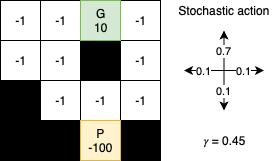
\includegraphics[scale=0.5]{images/MDPWorld.png}
  \caption{An example of an MDP world. White squares represent possible states. The agent can start from \textbf{any} of the white squares. There are 2 special terminal states: the green square represents the goal, and the yellow square represents the penalty state. Each state has an associated reward value which is collected whenever the agent leaves the state (for the terminal states, the reward is collected instantaneously). There are 4 possible actions (up, right, down, left; 4-point connectivity), but each action is stochastic meaning that if the agent chooses a specific direction it will move in that direction with 0.7 probability or it will move to the other directions with equal probability}
  \label{fig:MDPWorld}
\end{figure}

$R_t$ represents the total discounted reward from time step $t$, and it is defined in terms of the collected rewards $r_t$.

$$R_t = r_{t+1} + \gamma r_{t + 2} + \gamma^2 r_{t + 3} + ... = \sum_{k = 0}^{\infty} \gamma^k r_{t + k + 1}$$

The value function $V^{\pi}(s)$, where $\pi$ is the policy,  with signature $V^{\pi} \colon \mathcal{S} \xrightarrow{} \mathbb{R}$ represents a method for assessing how "good" a state is. It is defined as the expected total discounted reward.

$$V^{\pi}(s) = \mathbb{E}_{\pi}[R_t|S_t = s] = \sum_{a \in \mathcal{A}} \pi(s, a) \sum_{s' \in S} \mathcal{P}_{s, s'}^a (\mathcal{R}_{s, s'}^a + \gamma V^{\pi}(s'))$$

The state-action value function $Q^{\pi}(s, a)$ with signature $Q^{\pi} \colon \{ \mathcal{S}, \mathcal{A} \} \xrightarrow{} \mathbb{R}$ represents a method for assessing how "good" a state is, given a certain action.

$$Q^{\pi}(s, a) = \mathbb{E}_{\pi}[R_t|S_t = s, A_t = a] = \sum_{s' \in S} \mathcal{P}_{s, s'}^a (\mathcal{R}_{s, s'}^a + \gamma V^{\pi}(s'))$$

This also means that we can define $V^{\pi}(s)$ in terms of $Q^{\pi}(s, a)$.

$$V^{\pi}(s) = \sum_{a \in \mathcal{A}} \pi(s, a) Q^{\pi}(s, a)$$

\begin{Theo}{Bellman Optimality Equation}{Bellman}
The Bellman Optimality Equation states that the optimal value function is given by the following formula:
\begin{align*}
    V^{\pi^{*}}(s) &= \max_{a} \sum_{s' \in S} \mathcal{P}_{s, s'}^a (\mathcal{R}_{s, s'}^a + \gamma V^{\pi^{*}}(s')) = \max_{a} Q^{\pi^{*}}(s, a)\\
    Q^{\pi^{*}}(s, a) &= \sum_{s' \in S} \mathcal{P}_{s, s'}^a (\mathcal{R}_{s, s'}^a + \gamma V^{\pi^{*}}(s'))
\end{align*}
\end{Theo}

By following the Bellman Optimality Equation (\Cref{Th:Bellman}), we can devise a dynamic programming algorithm called Value Iteration. The algorithm updates $\mathcal{V^{\pi}}$ in place by applying the Bellman Optimality Equation for each state, thus finding better $\mathcal{V^{\pi}}$ on each run. We repeat the process until we see no further changes in $\mathcal{V^{\pi}}$. This means that $\mathcal{V^{\pi}}$ has converged for all $s \in \mathcal{S}$. After that, we return the optimal policy by choosing the optimal action at each state $s \in \mathcal{S}$ (See Algorithm \ref{alg: value_iteration}). If we run the algorithm on the MDP world defined in Figure \ref{fig:MDPWorld}, we will get the results presented in Figure \ref{fig:MDPResults}.

\begin{figure}[h!]
  \centering
  \begin{subfigure}[b]{0.3\linewidth}
    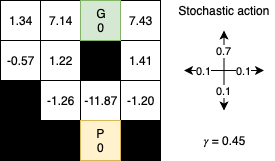
\includegraphics[width=\linewidth]{images/MDPWorldResult.png}
     \caption{Optimal value function}
  \end{subfigure}
  \hspace{1.3cm}
  \begin{subfigure}[b]{0.3\linewidth}
    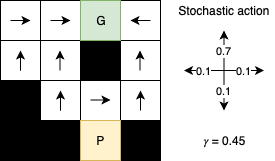
\includegraphics[width=\linewidth]{images/MDPWorldResultPolicy.png}
     \caption{Optimal policy}
  \end{subfigure}
  \caption{The results after applying the Value Iteration algorithm on the MDP World defined in figure \ref{fig:MDPWorld}. On the left, each cell contains the optimal value function $V^{\pi}(s)$. The optimal policy is displayed on the right}
  \label{fig:MDPResults}
\end{figure}

\begin{algorithm}
\caption{Value Iteration}
\label{alg: value_iteration}
\begin{algorithmic}[1]
\Procedure{Value-Iteration}{$\mathcal{S}$, $\mathcal{A}$, $\mathcal{P}$, $\mathcal{R}, \gamma$}
    \State Initialize $\mathcal{V^{\pi}}$, $\pi$ arbitrarily (e.g. all 0)
    \State
    \Repeat
        \For {\textbf{each} $s \in \mathcal{S}$}
            \State $V^{\pi}(s) = \underset{a \in \mathcal{A}}{\max} \hspace{0.1cm} \sum_{s' \in S} \mathcal{P}_{s, s'}^a (\mathcal{R}_{s, s'}^a + \gamma V^{\pi}(s'))$
        \EndFor
    \Until we have no change in $\mathcal{V^{\pi}}$
    \State
    
    \For {\textbf{each} $s \in \mathcal{S}$}
        \State $\pi(s) = \argmax{a \in \mathcal{A}}{\sum_{s' \in S} \mathcal{P}_{s, s'}^a (\mathcal{R}_{s, s'}^a + \gamma V^{\pi}(s'))}$
    \EndFor
    \State \textbf{return} $\pi$
\EndProcedure
\end{algorithmic}
\end{algorithm}

The time complexity is $\mathcal{O}(c|S||\mathcal{A}|)$ and the space complexity is $\mathcal{O}(|S|)$, where $c$ is the convergence rate, $|S|$ is the number of states and $|\mathcal{A}|$ is the number of actions. The time complexity is given by the update rule (which is $\mathcal{O}(|S||\mathcal{A}|)$, for each state we find the maximising action) being run $c$ times (some notebooks state that $c$ is bounded by $|S|$) and the final policy evaluation (which is still $\mathcal{O}(|S||\mathcal{A}|)$). The space complexity is given by the number of elements in $\mathcal{V^{\pi}}$ and $\pi$, which is the number of states $|S|$.

The advantage of using MDPs is that we can model a more complex world for the agent in which we can define areas which should be avoided (such as bridges, because they draw more battery power) by associating a negative reward with them. However, it can also be considered a disadvantage for worlds that cannot be easily modelled, as we have to know the transition probabilities and rewards apriori before we can apply Value Iteration. Not to mention that the number of states can get quite big. For instance, let us assume that we have a robotic arm with 3 joints, and each join can rotate 180\degree. If we discretise each angle into 1\degree angles, we will have a total number of $180^3 \simeq 5.8$ million states. There exist algorithms which can handle a large number of states such as Monte Carlo (sampling episode traces) and Temporal Difference Learning (combines dynamic programming and sampling), but we will not cover them as they are out of the report's scope \cite{szepesvari2010algorithms}.

\section{Sampling Based Planners} \label{B. Sampling based planners}
A significant drawback of using resolution complete (the algorithm is guaranteed to find a path) and resolution optimal (the algorithm will find the shortest path if one is available) graph search planners such as A*, is that they are only suitable for small problem sizes \cite{gammell2014informed}.

The algorithms described in this chapter employ a sampling technique to explore the unknown environment rapidly, thus scaling well with large problem sizes.

\subsection{Rapidly-exploring Random Tree (RRT)} \label{sec: RRT}
The Rapidly-exploring Random Tree (RRT) \cite{lavalle1998rapidly, rodriguez2006obstacle, lavalle2001randomized, karaman2011sampling} is a randomised data structure solution to the pathfinding problem which shares some desirable properties with probabilistic road-maps (PRM) \cite{choset2005principles}, but, unlike PRMs, it is able to handle problems that have non-holonomic constraints (a holonomic robot is a robot which is able to move instantaneously in all available degrees of freedom).

The algorithm starts by creating a graph $G$ with a single vertex containing the agent position. Then, we proceed to incrementally add new vertices until we get to the goal region (the region in which we can assume that we have reached the goal or will be able to safely reach it). At each iteration, we sample a new point on the map which represents a valid position (not intersecting any obstacle, or out of bounds) $x_{rand} \notin Os$. We find the nearest vertex $x_{near}$ from $x_{rand}$ by searching the graph (e.g. graph pruning). We choose the next vertex to be inserted $x_{new}$ based on a predefined $max\_dist$ variable. If we are too far from $x_{near}$ ($d(x_{near}, x_{rand}) > max\_dist$) we choose a point on the line segment defined by $x_{near}$ and $x_{rand}$ that is $max\_dist$ far away from $x_{near}$. If we are too close to $x_{near}$ ($d(x_{near}, x_{rand}) \leq max\_dist$) we simply choose $x_{rand}$ (See Figure \ref{fig:RRT_new_node}). After we have chosen $x_{new}$, we make sure that the path from $x_{near}$ to $x_{new}$ is collision free, and if it is we add $x_{new}$ as a new vertex to the graph $G$ and $(x_{near}, x_{new})$ as a new edge (See Figure \ref{fig:RRT_example}, See Algorithm \ref{alg: RRT}).

It is worth mentioning that there exist some variations which use a dynamic $max\_dist$, usually picking a random number from the interval $[0, max)$ at each new iteration. Furthermore, the algorithm can be extended to different metric spaces by changing the distance function $d$.

\begin{figure}[]
  \centering
  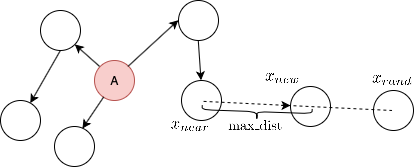
\includegraphics[scale=0.4]{images/RRT_new_node.png}
  \caption{RRT $x_{new}$ decision algorithm, if $x_{rand}$ is too far from $x_{near}$ we interpolate $x_{new}$ between the line segment defined by $x_{near}$ and $x_{rand}$ such that $x_{new}$ is $max\_dist$ away from $x_{near}$}
  \label{fig:RRT_new_node}
\end{figure}

\begin{figure}[]
  \centering
  \begin{subfigure}[b]{0.3\linewidth}
    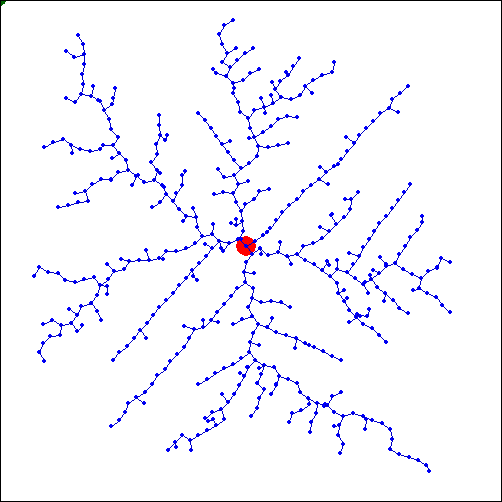
\includegraphics[width=\linewidth]{images/screenshot_40.png}
     \caption{500 iterations}
  \end{subfigure}
  \hfill
  \begin{subfigure}[b]{0.3\linewidth}
    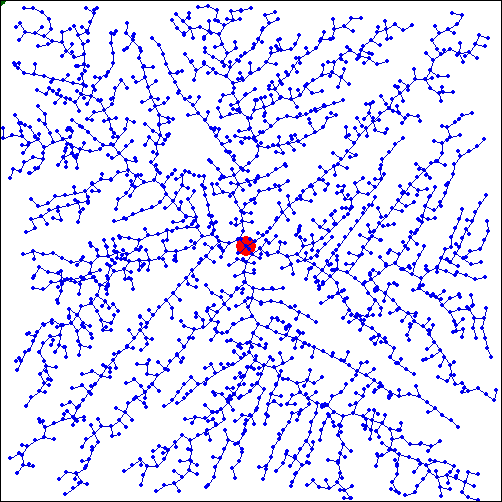
\includegraphics[width=\linewidth]{images/screenshot_41.png}
     \caption{2000 iterations}
  \end{subfigure}
  \hfill
  \begin{subfigure}[b]{0.3\linewidth}
    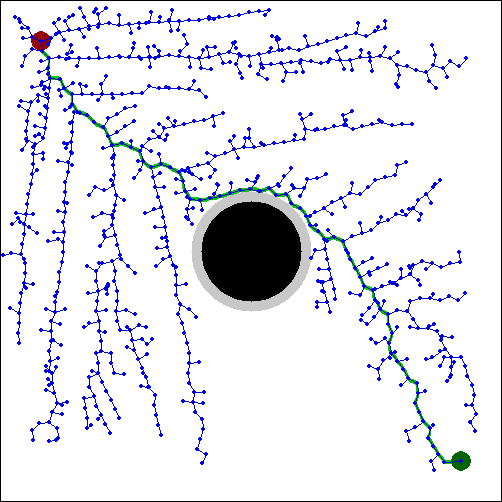
\includegraphics[width=\linewidth]{images/screenshot_39.png}
     \caption{Full RRT}
  \end{subfigure}
  \caption{RRT run with 500 iterations (left) and with 2000 iterations (middle) with $max\_dist$ 10. The whole algorithm can be seen in the right figure. Blue dots represent vertices and blue lines represent edges}
  \label{fig:RRT_example}
\end{figure}

\begin{algorithm}
\caption{Rapidly-exploring Random Tree (RRT)}
\label{alg: RRT}
\begin{algorithmic}[1]

\Procedure{RRT}{$M\colon(A, Os, G)$}
    \State $max\_dist \gets$ maximum distance
    allowed between tree children and sample
    \State $G \gets$ initalize graph with $A$ as vertex
    \While {True}
        \State $x_{rand} \gets \textit{Sample}()$
        \State $x_{near} \gets \textit{GetNearestVertex}(x_{rand})$
        \State $x_{new} \gets \textit{GetNewVertex}(x_{near}, x_{rand}, max\_dist)$
        \State
        \If {$\textit{CollisionFree}(x_{near}, x_{new})$}
            \State add $x_{new}$ as a new vertex to $G$
            \State add $(x_{near}, x_{new})$ as a new edge to $G$
        \EndIf
        \State
        \If {$x_{new}$ is in $G$ region}
            \State follow trace from root $G$ to $x_{new}$
            \State \Return 
        \EndIf
    \EndWhile
\EndProcedure
\end{algorithmic}
\end{algorithm}

Space complexity is $\mathcal{O}(|V| + |E|)$, where $|V|$ is the number of nodes and $|E|$ is the number of edges in graph $G$. Time complexity is given by $\mathcal{O}(i (\mathcal{O}(Sample) + \mathcal{O}(GetNearestVertex) + \mathcal{O}(GetNewVertex) + \mathcal{O}(CollisionFree)))$, where $i$ is the number of iterations and $\mathcal{O}(x)$ is the time complexity of method $x$. $i$ can be bounded by the number of nodes from graph $G$ ($\mathcal{O}(|V|)$) (at each step we add a new node to the graph). $\mathcal{O}(Sample)$ depends on the choice of sampling method (we use uniform random sampling which is $\mathcal{O}(1)$). $\mathcal{O}(GetNearestVertex)$ has DFS time and space complexity which is $\mathcal{O}(b^d)$ and $\mathcal{O}(bd)$, where $b$ is branching factor and $d$ is depth (if pruning is used $b$ becomes $\hat{b}$). $\mathcal{O}(GetNewVertex)$ is $\mathcal{O}(1)$ as it is a simple logical decision. $\mathcal{O}(CollisionFree)$ depends on the collision detection system. There are collision systems that have $\mathcal{O}(n)$ time complexity (for all entities). Because we need to check the path between $x_{near}$ and $x_{new}$ we still have $\mathcal{O}(n)$ time complexity. Therefore, the final time complexity is given by $\mathcal{O}(|V|(\mathcal{O}(b^d) + \mathcal{O}(n)))$.

A major advantage of using this method is that it is quite fast and memory efficient since it is run on a subset of the grid (the samples). Moreover, the algorithm can be coupled with the algorithms described in the Section \ref {C. Interpolating curve planners} (\hyperref[C. Interpolating curve planners]{Interpolating Curve Planners}) by transforming the graph edges into curves, which offers support for non-holonomic robots.

A major disadvantage is that, although the algorithm is probabilistic complete (as more samples are drawn the more likely is to find a path to the goal), it does not find an optimal path and the solution is usually quite jerky.

To overcome this issues, we introduce the RRT* \cite{karaman2011sampling, gammell2014informed} algorithm which has been proven to be asymptotic optimal (as the number of iterations gets larger, the more we approach to the optimal solution). RRT* does this by incrementally modifying the structure of the graph. When a new node is affixed to the graph, the algorithm might choose to rewire the connections in the graph by considering the new node as a replacement parent for the other existing nodes, if the resulting change yields a better solution. 

A major drawback of using RRT* is that, in order to achieve an optimal solution, the number of iterations has to be quite large and therefore, it becomes quickly expensive in higher dimensions. The Informed RRT* \cite{karaman2011sampling} algorithm attempts to solve this issue by adopting an ellipsoid heuristic approach. The algorithm shares the same logic as RRT* and it only improves the performance of finding an optimal path once a solution is found. This is achieved by sampling from the ellipsoidal heuristic. Thus, the number of iterations is reduced, and the optimal search is focused on a smaller region.

% \subsection{RRT*}

% Therefore, we introduce the RRT* \cite{karaman2011sampling} algorithm which is asymptotic optimal (as the problem size gets bigger, the more we approach to the optimal solution).

% % - prefers exploring the unexplored regions, large vornoi gaps
% % - good sampling from a smooth pdf Poisson Disc Sampling
% % - single nearest-neighbour queries

% \subsection{Informed RRT*}
% The informed RRT* \cite{gammell2014informed}
% %\subsection{Basic Probabilistic Road Map (Basic PRM)}
\section{Interpolating Curve Planners} \label{C. Interpolating curve planners}

% \todo{Add more citations}

The algorithms that lie into this section are used in the local planning part of the pathfinding problem. They attempt to find a trajectory that fits a given global description of the path (such as way-points) by taking into account multiple parameters such as feasibility, comfort, vehicle dynamics and efficiency. Interpolation is used to increase the number of data points between the way-points in order to smooth out the trajectory and create easily traversable paths for non-holonomic robots \cite{gonzalez2016review}.

\textbf{Lines and Circles.} Primitives such as lines and circles can be used to describe the local path between two way-points. Figure \ref{fig:c_all_curve_planners}(a) represents the shortest path to execute a 3-step 180\degree turn for a car. Because it can only fit geometric primitives, the algorithm is simple to implement and fast, but it is also quite limited (preferential parameters such as curvature angle and continuation are completely ignored).

\textbf{Clothoid Curves.} The implementation of this algorithm is based on Fresnel integrals, and the resulting curves offer a smoother transition between different curvatures (such as between a straight line and a curve) than Lines and Circles (See Figure \ref{fig:c_all_curve_planners}(b)). The algorithm accounts for multiple constraints such as dynamic and physical vehicle limitations (e.g. steering wheel), thus making it more robust for non-holonomic robots such as a car. Moreover, the algorithm was used in the design of highways and railways.

\textbf{Polynomial Curves.} This type of curves are mainly used to satisfy different preferential parameters such as angle and curvature when drawing the trajectory between two way-points. The main advantage of using this method is that the preferential parameters determine the coefficients of the polynomial, and thus, it is much more flexible. Figure \ref{fig:c_all_curve_planners}(c) represents an example of using polynomial curves to change lanes.

\textbf{Bézier Curves.} This algorithm produces curves based on control points. The control points placement defines the curvature at the beginning and the end of the curve.  The significant advantage of this algorithm is that it has a low computational cost since the shape of the curve is defined by the control points. Therefore, the algorithm has been extensively used in different drawing software applications, technical drawing (they can also be drawn by hand) and trajectory design. Moreover, the curve can be used to approximate clothoid curves. Figure \ref{fig:c_all_curve_planners}(d) represents an example of using 3rd and 4th degree Béziers to find the best curvature estimate based on the current situation.

\textbf{Spline Curves.} The spline curve is sub-divided into multiple parametric patches that can be defined as polynomial curves, clothoid curves and b-splines (Bézier curves). Splines have a high degree of smoothness at each patch joint and can be extended into higher dimensions. Figure \ref{fig:c_all_curve_planners}(e) represents an example of a b-spline with a changing knot (the junction between two sub-segments).

It is worth mentioning that the global description of the path demands to include the collision-free areas in addition to the way-points or provide a collision detection system to be used when drawing the curves to ensure that no collisions are encountered while performing any of the above algorithms.

\begin{figure}[h!]
  \centering
  \begin{subfigure}[b]{0.22\linewidth}
    \includegraphics[width=\linewidth]{images/c_lines_and_circles.png}
     \caption{Lines and Circles \cite{gonzalez2016review}}
  \end{subfigure}
  \hfill
  \begin{subfigure}[b]{0.33\linewidth}
    \includegraphics[width=\linewidth]{images/c_clothoid.png}
     \caption{Clothoid \cite{gonzalez2016review}}
  \end{subfigure}
  \hfill
  \begin{subfigure}[b]{0.38\linewidth}
    \includegraphics[width=\linewidth]{images/c_polynomial.png}
    \caption{Polynomial \cite{gonzalez2016review}}
  \end{subfigure}
  \newline
  \begin{subfigure}[b]{0.28\linewidth}
    \includegraphics[width=\linewidth]{images/c_bezier.png}
     \caption{Bézier \cite{gonzalez2016review}}
  \end{subfigure}
  \hspace{1cm}
  \begin{subfigure}[b]{0.33\linewidth}
    \includegraphics[width=\linewidth]{images/c_splines.png}
     \caption{Spline \cite{gonzalez2016review}}
  \end{subfigure}
  \caption{Examples of the most important interpolating curve planners}
  \label{fig:c_all_curve_planners}
\end{figure}
\section{Numerical Optimization Approaches} \label{D. Numerical optimization approaches}
This category of algorithms describes the path planning problem as a cost function, which is then minimised by using function approximation techniques and machine learning methods.

\subsection{Potential Field Method}
The main concept of the Potential Field Method (PFM) \cite{gonzalez2016review, ge2002dynamic, barraquand1992numerical} algorithm is to fill the map with a potential field $f$ in which the robot is attracted towards the goal and repulsed from obstacles. The potential field $f$ is composed of two functions: $f = a + r$ where $a$ is the attraction function and $r$ is the repulsion function. After the potential function is computed, an optimisation technique of finding the minimum of $f$, such as gradient descent, is applied (See Figure \ref{fig:pfm}). The Wave-front Planner \ref{sec: wave-front} is an example of a potential function $f=a$ where the repulsion function is missing.

The space complexity is $\mathcal{O}(nm)$ where $n$ is the width and $m$ is the height of the map. The time complexity is $\mathcal{O}(\mathcal{O}(f) + \mathcal{O}(gradient\_descent))$. $\mathcal{O}(f) = \mathcal{O}(\mathcal{O}(a) + \mathcal{O}(r))$ depends on the choice of $a$ and $r$. Assuming same $a$ as in the Wave-front Planner, $\mathcal{O}(a) = \mathcal{O}(b^d)$, where $b$ is the branching factor and $d$ is the depth. Assuming that we use a simple $r$ which inflates the obstacle, the time complexity of $\mathcal{O}(r)$ is $\mathcal{O}(xo)$, where $x$ is the inflation rate and $o$ is the average obstacle size. $\mathcal{O}(gradient\_descent)$ is more involved if we use real gradient descent optimisation as it is based on the convergence rate. If we were to use the same gradient descent method from the Wave-front Planner, then $\mathcal{O}(gradient\_descent) = \mathcal{O}(d)$, where $d$ is the depth of the solution. The final time complexity is $\mathcal{O}(b^d + xo + d)$.

This solution is appealing because it is mathematically elegant and simple. It behaves well on complex environments which contain narrow passages, and it keeps a safe distance from the obstacles based on different factors such as relative velocity. Moreover, the algorithm can be extended to highly dynamic environments in which the obstacles and the goal are continually moving. Lastly, we can use vehicle parameters such as velocity and torque, to define $a$ and $r$. Thus, we can avoid collisions based on the velocity of the vehicle (i.e. when the vehicle has a high enough velocity to not being able to exit a collision trajectory) \cite{ge2002dynamic}.

One of the major drawbacks of using this method is that depending on the choice of $f$, local minimum problems might arise. Usually, these problems require particular solutions and rigorous analysis to ensure that there is no situation in which the agent will be trapped forever.

\begin{figure}[h!]
    \centering
    \includegraphics[scale=0.3]{images/pfm.png}
    \caption{Potential field $f = a + r$, where $a$ is the attraction function and $r$ is the repulsion function \cite{inproceedings}}
    \label{fig:pfm}
\end{figure}

\pagebreak

\subsection{LSTM}
Currently, the most important works that have considered LSTMs in this field are \cite{nicola2018lstm, lee2018lstm, inoue2019robot}.

%\cite{nicola2018lstm} uses an LSTM network to generate a path from the agent to the goal. The network was trained using A* on randomly generated maps and tested on maps from the online game Dragon Age. The issue with this approach is that the agent might get lost and will not succeed in finding a path to the goal, if there exists one. It has also been noticed that the algorithm has a higher success rate if the size of the map is relatively small and simple in layout.

Nicola et al. attempt to use an LSTM network to create an online global path planner by generating a low-resolution high-level path from start to goal \cite{nicola2018lstm}. The network was trained on randomly filled generated mazes with different corridor sizes with A* \ref{sec:a_star} as ground truth and tested on maps from the popular game Dragon Age. The primary motivation of using the proposed method from \cite{nicola2018lstm} is that, unlike A* which is offline (directly produces the final output), this method is an online search strategy that takes into account the fact that the environment is usually unknown or too expensive to store. Thus, at each time step, the network is queried for the next action that it should take given the local information of the map and previous choice of action. One of the significant drawbacks is that the rate of success of the algorithm gets lower as the map becomes more complicated (longer corridors, more complex objects).

Lee et al. make use of the LSTM architecture to extend the state of the art Value Iteration Networks (VIN) \cite{lee2018lstm}. VINs are similar to the Value Iteration algorithm described in \label{sec:vin} applied on a 2D grid world, but without making use of pre-defined MDP parameters such as the transition probabilities and rewards. The paper has pointed out that, despite being so successful, there are still issues with the current design of VIN such as the design of the transition model and the large number of recursive calls taken to achieve a reasonable estimate of the optimal path to the goal. The proposed solution replaces the recurrent VIN update rule with an LSTM kernel. \cite{lee2018lstm} has shown that the performance of the new solution has better or at least as good performance as the original VIN.

Inoue et al. aim to use a Convolutional Auto-encoder (CAE) combined with an LSTM to plan a path under a changing environment, by disregarding the unknown environment constraint (the map is fully discovered) \cite{inoue2019robot}. The two network sections are trained individually. Firstly, the CAE is trained on randomly generated maps with obstacles of different sizes. After that, the decoder is discarded, and the encoder is used to encode the same maps in order to extract the main features. Secondly, the LSTM is trained on the encoded maps by using RRT as ground truth. Unlike \cite{nicola2018lstm}, the solution is offline as it produces a full path (which might collide with obstacles), but it can be easily converted to an online solution in order to handle collision detection and prevention. A significant difference between this solution and \cite{nicola2018lstm} is that it has a higher overall success rate, which might arise since the CAE learns the input features as opposed to being hand crafted as in \cite{nicola2018lstm}.

%\cite{inoue2019robot} has a similar approach to \cite{nicola2018lstm}, but, in addition, it compares the LSTM network to a Value Iteration Network. The results show that the LSTM is, overall, better than the Value Iteration Network, but, still, they share the same issues as \cite{nicola2018lstm} (i.e. the algorithm has a low success rate of finding a path to the goal and if it finds one it is usually not optimal).


%\subsection{Machine Learning and Neural Networks methods}
%VIN (Value Iteration Networks)
%LSTMIN (Long Short Term Memory Iteration Networks)
\chapter{Background} \label{Background}

Machine Learning (ML) is a programming approach for creating Artificial Intelligence (AI) systems in non-trivial environments by making use of experiences and a substantial amount of data \cite{ml, Goodfellow-et-al-2016, russell2016artificial, lecun2015deep}. 

One of the most trivial Machine Learning examples is classifying handwritten digits by making use of the MNIST database \cite{mnist}. It is conspicuous that Machine Learning is the only viable option in developing this kind of applications as it is tough (if not impossible) to come up with hard-coded rules for each class case \cite{Goodfellow-et-al-2016}.

\textbf{Notation.} We will follow the same mathematic conventions used in \cite{Goodfellow-et-al-2016} (See Table \ref{tab: notations}).

% \begin{itemize}
%     \item $x$ - A scalar 
%     \item $\boldsymbol{x}$ - A vector 
%     \item $\boldsymbol{M}$ - A matrix 
%     \item $\boldsymbol{M}^T$ - A transposed matrix
%     \item $x_{i}$ - Element $i$ from vector % $\boldsymbol{x}$, starting from 0
%     \item $\boldsymbol{X}_{i}$ - Row $i$ of matrix % $X$
%     \item $X_{i, j}$ - The element with row $i$ and % column $j$ from matrix $X$
%     \item $\boldsymbol{x} * \boldsymbol{y}$ - An % element-wise vector product
% \end{itemize}

\begin{table}[h!]
    \centering
    \begin{tabular}{l l}
        $x$ & A scalar \\
        $\boldsymbol{x}$ & A vector \\
        $\boldsymbol{M}$ & A matrix \\
        $\boldsymbol{M}^T$ & A transposed matrix \\
        $x_{i}$ & Element $i$ from vector $\boldsymbol{x}$, starting from 0 \\
        $\boldsymbol{X_{i}}$/$\boldsymbol{x_{i}}$ & Row $i$ of matrix $\boldsymbol{X}$ \\
        $X_{i, j}$ & The element with row $i$ and column $j$ from matrix $\boldsymbol{X}$ \\
        $\boldsymbol{x} * \boldsymbol{y}$ & An element-wise vector product \\
        $x^{(l)}$/$\boldsymbol{x^{(l)}}$/$\boldsymbol{X^{(l)}}$ & Depends on the context of $l$ \\
    \end{tabular}
    \caption{Notations \cite{Goodfellow-et-al-2016}}
    \label{tab: notations}
\end{table}

The aim of Machine Learning methods is to find a pattern in the features of data $\boldsymbol{X} \in \mathbb{R}^{n \times m}$, where $n$ is the number of data examples and $m$ is the number of features. Machine Learning can be classified into two major categories: supervised and unsupervised, but we are going to focus on supervised ML. Supervised ML operates on data that has been labelled with $\boldsymbol{y} \in \mathbb{R}^{n}$, where each $y_i$ corresponds to a row in $\boldsymbol{X}$, $f(\boldsymbol{x_i}) = y_i$, $f \colon \mathbb{R}^m \xrightarrow{} \mathbb{R}$. Our goal is to find a function $h \colon \mathbb{R}^m \xrightarrow{} \mathbb{R}$ which approximates $f$, $h(\boldsymbol{x_i}) \simeq f(\boldsymbol{x_i})$.

\section{Neural Networks}
(Feed-forward) Neural Networks (NN) \cite{ml, Goodfellow-et-al-2016, russell2016artificial, lecun2015deep} are a type of supervised Machine Learning inspired by real-world biological neurons. Each NN architecture is composed of artificial neurons.

\subsection{Artifical Neuron}

An artificial neuron \cite{ml, russell2016artificial, Goodfellow-et-al-2016} (See Figure \ref{fig:artificial_neuron}) has $m + 1$ inputs $x_{i \in \{0, ..., m\}}$ and $m + 1$ weights $w_{i \in \{0, ..., m\}}$, where input $0$ is a bias (we set $x_0 = 1$ so that $w_0$ becomes bias), with one output $y$. The neuron can be "activated" using an activation function $f$ such as sigmoid ($\sigma(x) = \frac{1}{1 + e^x}$), tanh ($tanh(x) = \frac{e^x - e ^{-x}}{e^x + e ^{-x}}$) or rectified linear unit (ReLU) ($f(x) = \begin{cases} 0, x < 0 \\ x, x \geq 0 \end{cases}$). The big picture is that the weights help the neuron learn a combination of inputs while the bias behaves like a learnable threshold. The idea behind the activation function is that we can define if a neuron is active or non-active based on the output value of $f$ (e.g. for sigmoid $f\colon \mathbb{R} \xrightarrow{} [0, 1]$, if $f < 0.5$ neuron is non-active).

$$y = f(z) = f(\sum_{i = 0}^{m} x_i \cdot w_i) = f(\boldsymbol{x}^T \boldsymbol{w}), x_0 = 1 \text{ and } w_0 \text{ bias}$$

\begin{figure}[h!]
  \centering
  \includegraphics[scale=0.4]{images/artificial_neuron.png}
  \caption{Artificial neuron representation}
  \label{fig:artificial_neuron}
\end{figure}

\subsection{Neural Network Architecture}

We can then combine multiple artificial neurons to create a layered architecture (See Figure \ref{fig:nn}). There are 3 types of layers: the input layer, the output layer and the hidden layer. The input and output layers are mandatory and should match the number of neurons with the size of the input features and respectively output. The number of hidden layers, as well as, their number of neurons are part of the NN architecture, and they are referred to as the depth and respectively the width of the network \cite{ml, russell2016artificial, Goodfellow-et-al-2016}.

\begin{figure}[h!]
  \centering
  \includegraphics[scale=0.4]{images/nn.png}
  \caption{Neural network architecture with 2 hidden layers}
  \label{fig:nn}
\end{figure}

\subsection{Forward-propagation}

Each layer can be then written as $\boldsymbol{a^{(l)}} = f(\boldsymbol{z^{(l)}}) = f(\boldsymbol{W^{(l)}}^T \boldsymbol{a^{(l - 1)}})$, where
$\boldsymbol{a^{(l - 1)}} \in \mathbb{R}^{m + 1}$ is the input to layer $l$,
$\boldsymbol{a^{(l)}} \in \mathbb{R}^d$ is the output of layer $l$,
$\boldsymbol{W^{(l)}} \in \mathbb{R}^{(m + 1) \times d}$ are the weights associated with layer $l$, 
$a^{(l - 1)}_{0} = 1$ and
$\forall i.W^{(l)}_{i, 0}$ is bias. Therefore, each row $r$ in $\boldsymbol{W^{(l)}}$ corresponds to the weights associated with the $r$ neuron in layer $l$. $l = 0$ corresponds to the input layer and $l = L$ is the output layer. Now, we can write the whole architecture as following:

\begin{align*}
    \boldsymbol{y} &= \boldsymbol{a_{L}} \\
    \boldsymbol{a_{0}} &= \boldsymbol{x} \\
    \boldsymbol{a^{(l)}} &= f(\boldsymbol{W^{(l)}}^T \boldsymbol{a^{(l - 1)}}) \\
    \boldsymbol{y} &= f(\boldsymbol{W^{(L)}}^T f(\boldsymbol{W^{(L - 1)}}^T f(...f(\boldsymbol{W^{(0)}}^T \boldsymbol{x})))
\end{align*}

For now we can only (forward) propagate our input through the network and receive a random output, but we do not learn from our data $\boldsymbol{x}$ \cite{ml, russell2016artificial, Goodfellow-et-al-2016}.

\subsection{Back-propagation}

% The idea behind back-propagation is that when we are training the network, we would like to have a method for checking how good are we approximating the output against $\boldsymbol{y}$ and if we are not doing so great "learn" from it \cite{ml, russell2016artificial, Goodfellow-et-al-2016}.

Back-propagation \cite{ml, russell2016artificial, Goodfellow-et-al-2016} is a method in which we perform a backward pass through the network in order to adjust the weights of the neurons. The changing amount depends on how well we currently approximate the output against $\boldsymbol{y}$. If we have a bad approximation we adapt the weights in order to get closer to the true output.

We can develop a cost function $J$ that uses a loss function $L$ which will tell us how close are we to the actual solution. As an example, the least square error is a loss function used in regression $L(\boldsymbol{y^{(l)}}, \boldsymbol{a^{(l)}}) = \frac{1}{n} \sum^{n}_{i = 0} (y^{(l)}_i - a^{(l)}_i) ^ 2$, $J = L$. Our objective is to minimise the cost function $J$, as we would like to be as close as possible to the actual solution, while updating the weights (learn from our mistakes).

In order to update the weights correctly, we are going to use gradient descent (See Figure \ref{fig:learning_rate}), which is an iterative first-order method for finding a local minimum (or maximum as both problems are equivalent) or global minimum if the problem is convex. Therefore the update rule for our weights becomes:

\begin{align*}
    \boldsymbol{W^{(l)}} \gets \boldsymbol{W^{(l)}} - \alpha \frac{\partial J^{(l)}}{\partial \boldsymbol{W^{(l)}}}
\end{align*}

for each layer $l$, where $\alpha$ is the learning rate. The weights are updated starting from the output layer $l=L$ towards the input layer $l=0$ as when we update the layer $l=k$, we need the output of layer $l=k+1$ in order to compute $J^{(l)}$.

\subsection{Learning Rate}
The learning rate \cite{ml} $\alpha$ controls how much we change the weights. We have to be careful when setting the learning rate as if it is too low we might not reach the minimum (if we do not have enough iterations) or if it is too high, we are going to oscillate and might not find the minimum or even diverge (See Figure: \ref{fig:learning_rate}).

There are techniques that deal with this issue such as momentum or exact linear search optimisations for the learning rate: Golden Section or Newton-Raphson methods \cite{chong2013introduction}: 

$$\alpha^{(j)} \in \argmin{\alpha \geq 0} {\boldsymbol{W^{(l)}} - \alpha^{(j)} \frac{\partial J^{(l)}}{\partial \boldsymbol{W^{(l)}}}}\textrm{, for each iteration j}$$

\begin{figure}[]
  \centering
  \begin{subfigure}[b]{0.32\linewidth}
    \includegraphics[width=\linewidth]{images/gradient_descent_just_right.png}
     \caption{Learning rate is just right}
  \end{subfigure}
  \begin{subfigure}[b]{0.32\linewidth}
    \includegraphics[width=\linewidth]{images/gradient_descent_too_small.png}
     \caption{Learning rate is too small}
  \end{subfigure}
  \begin{subfigure}[b]{0.32\linewidth}
    \includegraphics[width=\linewidth]{images/gradient_descent_too_high.png}
     \caption{Learning rate is too high}
  \end{subfigure}
  \caption{Gradient descent with a reasonable, too small or too high learning rate. When the learning rate is reasonable we reach a minimum point, when the learning rate is too small we do not reach a minimum if the number of iterations is not high enough, and when the learning rate is too high we start to oscillate and might even diverge}
  \label{fig:learning_rate}
\end{figure}
\subsection{Training}
Putting it altogether, in order to train the Neural Network, for each training example $\boldsymbol{x_i}$ we:
\begin{itemize}
    \item execute a forward propagation to get $\forall l \in \{0, ..., L\}.\boldsymbol{a^{(l)}}$
    
    \item back-propagate to update the weights $\forall l \in \{0, ..., L\}.\boldsymbol{W^{(l)}}$ following the gradient descent formula
\end{itemize}

However, before training the model, we have to process the data so that we have a mechanism of improving (by tuning the hyper-parameters) and evaluating the model. There are multiple ways of splitting the data, but we are going to focus on the most important ones: holdout and $k$-fold cross validation \cite{ml, russell2016artificial, Goodfellow-et-al-2016}.

The holdout method is mostly used when there is a lot of training data. The training data is split into three subsets: training, validation and testing (usually 60\% training, 20\% validation, 20\% testing). The model is then trained on the training data and evaluated on the validation data in order to improve the performance of the network by tuning the model hyper-parameters. The process of passing the entire training and validation data through the model is known as an epoch. The process can then be repeated $n$ epochs until no further improvement is noticed or over-fitting occurs. When the model is tuned, we run a final evaluation on the testing data to report the final results of our model. We do not tune the model on the testing data as this would contradict our generalisation assumption and will make the evaluation redundant.

In the case of having low amounts of training data, we can opt for the $k$-fold cross validation method. The idea behind this method is that we are going to partition our data set into two groups: training and testing $k$ times. The partitioning is achieved as seen in Figure \ref{fig:cross_fold}. The training process is similar to the holdout method, but the evaluation results are averaged over the splits. It is worth mentioning that there are many variants to this method such as: leave $n$ out, leave one out, $k$-fold cross validation with validation and test set and many more.

\begin{figure}[h!]
  \centering
  \includegraphics[scale=0.5]{images/cross_fold.png}
  \caption{$k$-fold cross validation. Training data is represented with green and testing data is represented with red}
  \label{fig:cross_fold}
\end{figure}


\subsection{Evaluation}
At each evaluation step in our training pipeline, we can report a series of useful statistical measures such as loss over model complexity, precision, accuracy, recall, $F_1$ measure, confusion matrices and others \cite{ml, russell2016artificial, Goodfellow-et-al-2016}.

\subsection{Over-fitting}
Over-fitting \cite{ml, russell2016artificial, Goodfellow-et-al-2016} occurs when the model's predictions are almost perfectly matching the training data targets, meaning that it cannot generalise for unseen data. The opposite phenomenon is under-fitting and happens when the model is under-trained and cannot make any useful predictions. Formally, when the model under-performs, it has high bias, and when the model over-performs, it has high variance (See Figure \ref{fig:overfit}).

\begin{figure}[h!]
  \centering
  \includegraphics[scale=0.32]{images/overfit.png}
  \caption{Over-fitting example. Blue dots represent the actual function we are trying to approximate, the red function is just right, the green function is over-fitting, the blue function is under-fitting. The model was trained on the interval $[0, 0.9]$}
  \label{fig:overfit}
\end{figure}

Over-fitting starts at the point where the cost function starts increasing on the testing data, even though it keeps decreasing on the training data (See Figure \ref{fig:overfit_thresh}).

\begin{figure}[h!]
  \centering
  \includegraphics[scale=0.6]{images/overfit_tresh.png}
  \caption{Over-fitting threshold}
  \label{fig:overfit_thresh}
\end{figure}

\subsection{Regularisation}
To overcome the over-fitting problem we can use different approaches such as: early stopping (manually stop the training process when over-fitting is spotted), dropout (assign a probability that a neuron will "fire"), adding noise to data, L-norm regularisation (add a penalty term to the loss function; e.g. L1, L2, max norm) \cite{ml, russell2016artificial, Goodfellow-et-al-2016}.

L1 regularisation is used to "get rid" of weights by effectively setting them to 0. Intuitively, this means that we are going to only keep meaningful features.

$$J(\boldsymbol{W}) = L(\boldsymbol{y}, \boldsymbol{a}) + \lambda \sum_{w} |w|\textrm{, where $\lambda$ is the regularisation factor}$$

L2 regularisation is used to "punish" large weights, thus favouring small weights. This means that our $h$ will not oscillate that much due to high weights. It should be noted that L2 is more sensible to outliers than L1.

$$J(\boldsymbol{W}) = L(\boldsymbol{y}, \boldsymbol{a}) + \lambda \sum_{w} w^2\textrm{, where $\lambda$ is the regularisation factor}$$

\section{Recurrent Neural Networks}
Neural Networks are great for solving regression, logistic and classifying problems, but they do not handle well time-series problems. One of the reasons why is that time-series problems depend on the previous state and due to the acyclic graph design of the NN architecture, this information cannot be propagated through the network, and it is lost.

Recurrent Neural Networks (RNN) \cite{ml, LSTM_blog} are tackling this sort of issue by introducing a backwards edge from the last hidden layer to the first hidden layer in the NN architecture that carries the previous state information. Thus, if we unfold the RNN architecture, we can notice that each previous outcome is connected to the current one (See Figure \ref{fig:RNN}).

\begin{figure}[h]
  \centering
  \includegraphics[scale=0.30]{images/RNN-unrolled.png}
  \caption{Recurrent Neural Network \cite{LSTM_blog}}
  \label{fig:RNN}
\end{figure}

One of the major issues with RNNs is that they do not train well. They use back-propagation through time, which is a similar training process to the NN one, but it achieved over the length of the time series. This procedure suffers from the vanishing or exploding gradient problem. The vanishing gradient problem states that if the gradient of the weights is less than 1 at time $t$, than as $t \xrightarrow{} 0$ so is $\nabla w^{(t)} \xrightarrow{} 0$. In the case of the weights being matrices, we use the L2 norm $\left\lVert \nabla \boldsymbol{W^{(t)}} \right\rVert = \sqrt{\lambda}$, where $\lambda$ is the largest eigenvalue of $\boldsymbol{W^{(t)}}$. The exploding gradient problem states that if the gradient of the weights is greater than 1 at time $t$, than as $t \xrightarrow{} 0$, $\nabla w^{(t)} \xrightarrow{} \infty$ (analogue for $\boldsymbol{W^{(t)}}$). Therefore, only the first layers from the back are trained properly if the time-series length is even remotely big. A common solution (but not preferred) to this problem is to change the architecture by adding extra backward edges between hidden layers so that we can propagate the gradient more efficiently.

\section{Long Short-Term Memory (LSTM)}
The Long Short-Term Memory (LSTM) \cite{hochreiter1997long, LSTM_blog} is a type of Recurrent Neural Network that solves the vanishing and exploding gradient problem by adding internal gates to the architecture to control the gradient flow during training.

As seen in Figure \ref{fig:LSTM}, the LSTM cell contains four types of internal gates that control the flow of information, and three types of input: $\boldsymbol{x^{(t)}}$ (the actual input at time $t$), $\boldsymbol{c^{(t)}}$ (cell state at time $t$, which we do not expose outside the internal architecture) and $\boldsymbol{h^{(t)}}$ (hidden state at time $t$).

\begin{figure}[h]
  \centering
  \begin{subfigure}[b]{0.6\linewidth}
    \includegraphics[width=\linewidth]{images/lstm_archi_cell.png}
  \end{subfigure}
  \hfill
  \begin{subfigure}[b]{0.6\linewidth}
    \includegraphics[width=\linewidth]{images/LSTM2-notation.png}
  \end{subfigure}
  \caption{LSTM cell \cite{LSTM_blog}}
  \label{fig:LSTM}
\end{figure}

The \textbf{forget} gate $\boldsymbol{f^{(t)}} = \sigma(\boldsymbol{W^{(f)}} \cdot [\boldsymbol{h^{(t - 1)}}, \boldsymbol{x^{(t)}}] + \boldsymbol{b^{(f)}})$, where $\sigma$ is the sigmoid function, $\boldsymbol{W^{(f)}}$ are the weights and $\boldsymbol{b^{(f)}}$ is the bias associated with the \textbf{forget} gate, controls the amount of information that we would like to forget as $\boldsymbol{f^{(t)}} \colon \mathbb{R}^n \xrightarrow{} [0, 1]$, so when $\boldsymbol{f^{(t)}}$ tends to 0 we forget more about the previous states.

The \textbf{input} gate $\boldsymbol{i^{(t)}} = \sigma(\boldsymbol{W^{(i)}} \cdot [\boldsymbol{h^{(t - 1)}}, \boldsymbol{x^{(t)}}] + \boldsymbol{b^{(i)}})$ controls how much information we would like to keep from the input. As in the case of the \textbf{forget} gate, when $\boldsymbol{i^{(t)}}$ tends to 0 we discard more information.

The \textbf{gate} gate $\boldsymbol{g^{(t)}} = tanh(\boldsymbol{W^{(g)}} \cdot [\boldsymbol{h^{(t - 1)}}, \boldsymbol{x^{(t)}}] + \boldsymbol{b^{(g)}}$ decides the importance of the data. Because $\boldsymbol{g^{(t)}}\colon \mathbb{R}^n \xrightarrow{} [-1, 1]$, if $\boldsymbol{g^{(t)}}$ tends to 1 we consider the input to be more important.

The next cell state is given by $\boldsymbol{c^{(t)}} = \boldsymbol{f^{(t)}} * \boldsymbol{c^{(t - 1)}} + \boldsymbol{i^{(t)}} * \boldsymbol{g^{(t)}}$. The cell state combines the output of all internal gates and contains the information that should be carried to the next state.

The \textbf{output} gate $\boldsymbol{o^{(t)}} = \sigma(\boldsymbol{W^{(o)}} \cdot [\boldsymbol{h^{(t - 1)}}, \boldsymbol{x^{(t)}}] + \boldsymbol{b^{(o)}})$ controls how much information we show to the user. As in the case of the \textbf{forget} and \textbf{input} gates, if $\boldsymbol{o^{(t)}}$ tends to 0 we output less information.

The actual output is given by the hidden state $\boldsymbol{h^{(t)}} = \boldsymbol{o^{(t)}} * tanh(\boldsymbol{c^{(t)}})$.

The particular design of this architecture solves the vanishing and exploding gradient problems by making use of the internal cell state $\boldsymbol{c^{(t)}}$. During training, the gradients flow more efficiently along the line defined between $\boldsymbol{c^{(t - 1)}}$  and $\boldsymbol{c^{(t)}}$. Moreover, it can be further extended by adding more LSTM layers by connecting the output at each time step from layer $n - 1$ to the input of layer $n$ to create a stacked architecture that has a similar effect to a Deep Neural Network.

It should be mentioned that there exist various LSTM architectures and extensions that attempt to improve the overall performance of the network such as: Gated Recurrent Units (GRUs), LSTMs with peephole connections and many more. Some of the extended architectures have reduced computational cost due to a lower complexity design (e.g. the GRU has a lower number of internal gates compared to the LSTM architecture), but, they still achieve similar or insignificantly better prediction performance than LSTMs \cite{ml, russell2016artificial, Goodfellow-et-al-2016, hochreiter1997long, LSTM_blog}.
\chapter{PathBench} \label{Simulation Platform}

PathBench is a motion planning platform used to develop, assess, compare and visualise the performance and behaviour of the discussed algorithms. The platform is split into four main components: \textbf{Simulator}, \textbf{Generator}, \textbf{Trainer} and \textbf{Analyzer} joined by the infrastructure section. Additionally, the platform provides a \textit{ROS} real-time extension for interacting with a real-world robot through PathBench (See Figure \ref{fig: sim_platform}). The full architecture can be seen in Figure \ref{fig:sim_architecture}. 

% the platform provides a \textit{ROS} real-time extension which integrates the \textit{gmapping} \textit{ROS} package (SLAM scan) into a dedicated internal map environment (\textbf{RosMap}) controlled by a master node (\textbf{Ros})

\textbf{Notation.} We will use \textit{italic font} for libraries, \textbf{bold font} for classes and \texttt{typewriter font} for code snippets/file names/functions/variables. For types, we use the \textit{python} type hinting system (e.g. a list of integers is defined as \texttt{List[int]}).

% \todo{Mention ROS extension and add ROS components in high overview}

% The \textit{ROS} section provides compatibility with the \textit{ROS} library by integrating the \textit{gmapping} package (SLAM scan) into an internal map environment (\textbf{RosMap}). The \textbf{Ros} component represents the master node which controls the interactions between the robot and PathBench. 

\begin{figure}[h!]
    \centering
    \includegraphics[scale=0.5]{images/sim_high_overview.png}
    \caption{PathBench structure high-overview. Arrows represent information flow/usage ($A \xleftarrow{gets/uses} B$). The Machine Learning section is responsible for training dataset generation and model training. The Environment section controls the interaction between the agent and the map, and supplies graphical visualisation. The \textit{ROS} section provides support for real-time interaction with a real physical robot. The Evaluation section provides benchmarking methods for algorithm assessment}
    \label{fig: sim_platform}
\end{figure}

\textbf{Infrastructure.} This component is responsible for linking all other components and provide general service libraries and utilities (for a comprehensive explanation of the infrastructure sub-components, please refer to Appendix \ref{sec: infra}).

\pagebreak

\textbf{Simulator.} This section is responsible for environment interactions and algorithm visualisation. It provides custom collision detection systems and a graphics framework for rendering the internal state of the algorithms.

\textbf{Generator.} This section is responsible for generating and labelling the training data used to train the Machine Learning models.

\textbf{Trainer.} This section is a class wrapper over the third party Machine Learning libraries. It provides a generic training pipeline based on the holdout method and standardised access to the training data.

\textbf{Analyzer.} The final section manages the statistical measures used in the practical assessment of the algorithms. Custom metrics can be defined as well as graphical displays for visual interpretations.

% the platform provides a \textit{ROS} real-time extension which integrates the \textit{gmapping} \textit{ROS} package (SLAM scan) into a dedicated internal map environment (\textbf{RosMap}) controlled by a master node (\textbf{Ros})

% The \textit{ROS} section provides compatibility with the \textit{ROS} library by integrating the \textit{gmapping} package (SLAM scan) into an internal map environment (\textbf{RosMap}). The \textbf{Ros} component represents the master node which controls the interactions between the robot and PathBench. 

\textbf{ROS Real-time Extension.} The extension provides real-time support for visualisation, coordination and interaction with a physical robot. The extension is split into two main components: \textbf{RosMap} (integrates the \textit{gmapping} \textit{ROS} package (SLAM scan) into a dedicated internal map environment) and \textbf{Ros (master node)}. We explain the \textbf{Ros (master node)} architecture and functionality in Section \ref{sec: robotexp} (\hyperref[sec: robotexp]{Path Planning on Real-world Robot}) in which we evaluate the performance of the proposed solution on a real robot.

\section{Comparison with other motion planner platforms}

Currently, there are a variety of standardised libraries which contain at least two of the mentioned sections (\textbf{Simulator} and \textbf{Analyzer}) such as: \textit{ROS} \cite{Quigley09}, \textit{OMPL} \cite{sucan2012the_open_motion_planning_library}, \textit{MoveIt} \cite{moveit} (has benchmarking capabilities \cite{moll2015benchmarking}).

\textbf{ROS.} The Robot Operating System (ROS) is a platform which contains various simulation environments (including 2D and 3D) for different types of robots: ground robots with different degrees of freedom constraints, flying robots (drones) and manipulator robots (arm robots which interact with different objects). It represents the standard library in robotics for simulation and development.

\textbf{OMPL.} The Open Motion Planning Library (OMPL) is a standalone library which focuses on motion planning exclusively. It is more lightweight than ROS and has reduced capabilities (there is no collision detection). The library of available path planners is limited to sampling-based planners such as RRT or PRM (probabilistic road maps), but there is a variety of optimised implementation for each type of planner.

\textbf{MoveIt.} Combines both ROS and OMPL to create a high-level implementation for cleaner and faster development of new algorithms. It has more capabilities than ROS and OMPL and includes custom benchmarking techniques \cite{moll2015benchmarking}.

\textbf{PathBench (our platform).} Our implementation offers a more abstract overview of the environment and is extremely lightweight compared to the mentioned libraries. We include both a simulation environment (\textbf{Simulator}) and benchmarking techniques (\textbf{Analyser}), but we also include a generator for creating synthetic datasets for Machine Learning applications (\textbf{Generator}) and a ML training pipeline (\textbf{Trainer}) for generic ML models. The \textbf{Analyser} is quite involved and extensible, but the \textbf{Simulator} has limited capabilities in both rendering and environment interaction compared to the other libraries. The main motivation of using our platform and not the existing standardised libraries is that the platform was build to be used in an ideal research environment. Since, we use ML methods, the focus was set on the path generation and not the interaction between the environment and the agent. However, we do provide a clean API interface for the algorithms which makes them portable to the standardised libraries. Moreover, we provide a \textit{ROS} real-time extension which converts the internal map move action into network messages (velocity control commands) using the \textit{ROS} publisher-subscriber APIs (See Table \ref{tab: plat_comparison} for platform comparison).

%\todo{SAJAD: A table showing features (support for ML, etc) vs platform (ROS, OMPLS, etc) would be the best fit for here.}

\begin{table}[h!]
    \footnotesize
    \centerfloat
    \begin{tabular}{|c|M{1.9cm}|M{2cm}|M{1.4cm}|M{1.9cm}|M{1.2cm}|M{1.8cm}|}
         \hline
         \textbf{Platform} & \textbf{Visualisation} & \textbf{Benchmarking} & \textbf{Machine Learning Support} & \textbf{Development Efficiency} & \textbf{Robot Variety} & \textbf{Environment Complexity and Interaction} \\
         \hline
         \textbf{ROS} & \checkmark & \xmark & \xmark & \textbf{Reduced} & \textbf{High} & \textbf{High} \\
         \hline
         \textbf{OMPL} & \checkmark & \xmark & \xmark & \textbf{High} & \textbf{Reduced} & \textbf{Reduced} \\
         \hline
         \textbf{MoveIt} & \checkmark & \checkmark & \xmark & \textbf{Moderate} & \textbf{High} & \textbf{High} \\
         \hline
         \textbf{PathBench} & \checkmark & \checkmark & \checkmark & \textbf{High} & \textbf{Reduced} & \textbf{Reduced} \\
         \hline
    \end{tabular}
    \caption{Platform capabilities comparison chart}
    \label{tab: plat_comparison}
\end{table}

\begin{figure}[h!]
    \centerfloat
    \includegraphics[scale=0.46]{images/simulator_architecture.png}
    \caption{Full platform architecture overview. Arrows with full head represent dependency ($A \xrightarrow{depends\, on/uses} B$) and arrows with hollow head represent inheritance ($A \xrightarrow{inherits\,from} B$). Colours are mapped as follows: purple is infrastructure, orange is simulator, green is generator, red is trainer, yellow is utility/analyser and white is extension}
    \label{fig:sim_architecture}
\end{figure}

\section{Implementation}

Before coding the platform, we have investigated a series of libraries and programming languages and we have decided to write it in \textit{python ver. 3.7.3}, use \textit{pytorch} \cite{paszke2017automatic} for machine learning and \textit{pygame} \cite{pygame} for rendering.

The choice of programming language was straightforward as \textit{python} is the standard in ML and research applications. Moreover, a lot of open source ML libraries are available such as \textit{tensorflow} \cite{tensorflow2015_whitepaper} and \textit{pytorch} which are used both in production software and researching.

For the ML library, we have chosen \textit{pytorch} over \textit{tensorflow}, because \textit{pytorch} was developed with the intent of it being used in research. \textit{tensorflow} is a mature ML library which has extensive community support, and it is used by major companies in production software, but, unlike \textit{pytorch}, it is quite hard to debug, due to the design of the computational graphs. In \textit{tensorflow}, you have to compile the model and use special session variables, while \textit{pytorch} offers the possibility of dynamically changing the computational graphs, which allows the user to debug more easily. This feature is most useful when dealing with RNNs with variable size inputs (in our case the LSTM) \cite{tensorflow_vs_pytorch}.

The simulator was build using the rendering library \textit{pygame}. The other choices included \textit{pyglet} \cite{pyglet} and \textit{Unity 3D} \cite{bartneck2015robot}. \textit{pyglet} is an advanced rendering engine which is based on \textit{OpenGL} \cite{opengl}, but due to the fact that we do not have graphics intensive requirements, a lightweight library such as \textit{pygame} is a better option. Moreover, \textit{pygame} provides useful rendering helper functions which do not require prior knowledge about \textit{OpenGL}, thus making development faster.

\textit{Unity 3D} was considered as an alternative to \textit{pygame} as it provides an additional physics engine which has collision detection and ray casting. Both features were needed in later development stages and had to be manually implemented. The main downside to choosing \textit{Unity 3D} was that we could not use \textit{pytorch} anymore, because \textit{Unity 3D} uses \textit{C\#} as the core programming language. There were multiple solutions to this issue: use \textit{IronPython}\footnote{\textit{IronPython} is a library which provides a \textit{python2} session wrapper that can be directly used in \textit{C\#} code} \cite{foord2009ironpython}, use the \textit{C\#} ML wrappers or create a ML server. However, none of them had a good trade-off to make the switch. Moreover, all solutions required different communication protocols which could have severely affected the performance of the path planners.

\section{Simulator}

The \textbf{Simulator} is both a visualiser tool and an engine for developing \textbf{Algorithm}s (See Figure \ref{fig: sim}). It supports animations and custom \textbf{MapDisplay} components which render the \textbf{Algorithm}'s internal data. Table \ref{tab: sim_commands} from Appendix \ref{sec: app_env} provides a list of user commands which control the simulator during run-time.

A \textbf{Map} contains different entities such as the \textbf{Agent}, \textbf{Goal} and \textbf{Obstacle}s, and provides a clean interface that defines the movement and interaction between them. Therefore, a \textbf{Map} can be extended to support various environments. The downside to this features is that each map has to implement its own physics engine or use a third party one (such as the \textit{pymunk} physics engine \cite{pymunk} or \textit{OpenAI Gym} \cite{OpenAI_Gym}). The current implementation supports three 2D maps: \textbf{DenseMap}, \textbf{SparseMap} and \textbf{RosMap}. 

The \textbf{DenseMap} stores entities in a grid format in order to reduce the time complexity of the APIs (i.e. collision detection, ray casting and line drawing). Collision detection is $\mathcal{O}(1)$, and most operations such as ray casting and line drawing are trivial to implement. When the agent has a radius attached to it, the obstacles are inflated by creating \textbf{ExtendedWall} objects around the obstacle boundary (the method is similar to the repulsion function from Potential Fields; time complexity is $\mathcal{O}(xo)$, where $x$ is the inflation rate and $o$ is the average obstacle size). The agent can overlap the \textbf{ExtendedWall} obstacles as long as the \textbf{ExtendedWall} obstacles do not contain its centre. 

Unlike the \textbf{DenseMap}, the \textbf{SparseMap} stores all entities in a list similar to \textit{Unity 3D}. It does not need obstacle inflation, and it has fast collision detection as only circles are used for each entity (circle collision is $\mathcal{O}(1)$), but it does not implement a pairwise checking algorithm (such as pairwise pruning or sweep and prune) and, thus, the complexity of the whole collision detection system becomes $\mathcal{O}(n^2)$ as all pairs of entities are checked. Thus, the \textbf{SparseMap} is mostly used to create user-defined maps which are then converted to a \textbf{DenseMap}.

% the platform provides a \textit{ROS} real-time extension which integrates the \textit{gmapping} \textit{ROS} package (SLAM scan) into a dedicated internal map environment (\textbf{RosMap}) controlled by a master node (\textbf{Ros})

% The \textit{ROS} section provides compatibility with the \textit{ROS} library by integrating the \textit{gmapping} package (SLAM scan) into an internal map environment (\textbf{RosMap}). The \textbf{Ros} component represents the master node which controls the interactions between the robot and PathBench.

%\todo{Talk about RosMap}
The \textbf{RosMap} extends the \textbf{DenseMap} to integrate the \textit{gmapping} \textit{ROS} package (SLAM scan) by converting the SLAM output image into an internal map environment. Because we extend the \textbf{DenseMap} component, we inherit the collision detection system and all additional functionality from it. The \textbf{RosMap} environment has support for live updates, meaning that algorithms can query an updated view by running a SLAM scan. The map uses simple callback functions to make SLAM update requests and convert movement actions into network messages using the \textit{ROS} publisher-subscriber communication system.

For all maps, movement is allowed in eight directions: horizontal, vertical and diagonal (movement cost is based on the Euclidean distance: horizontal/vertical 1 and diagonal $\sqrt{2}$). It should be noted that, because we are simulating the map environment, we need the full map information for \textbf{SparseMap} and \textbf{DenseMap}. However, because we provide a \textbf{Map} interface, we can define custom maps (such as \textbf{RosMap}) that restrict the agent information access (e.g. in the real world, the robot usually does not has access to the full information of the environment).

Additionally, the \textbf{Simulator} provides animations that are achieved through key frames and synchronisation primitives (the process is described in Appendix \ref{sec: infra}).

\begin{figure}[h]
  \centering
  \begin{subfigure}[b]{0.2\linewidth}
    \includegraphics[width=\linewidth]{images/screenshot_43.png}
     \caption{Wave-front planner (\ref{sec: wave-front})}
  \end{subfigure}
  \hfill
  \begin{subfigure}[b]{0.2\linewidth}
    \includegraphics[width=\linewidth]{images/screenshot_44.png}
    \caption{A* (\ref{sec:a_star}) \newline}
  \end{subfigure}
  \hfill
  \begin{subfigure}[b]{0.2\linewidth}
    \includegraphics[width=\linewidth]{images/screenshot_46.png}
     \caption{Dijkstra (\ref{sec: dijkstra}) \newline}
  \end{subfigure}
  \hfill
  \begin{subfigure}[b]{0.2\linewidth}
    \includegraphics[width=\linewidth]{images/screenshot_47.png}
     \caption{Bug 1 (\ref{sec: bug1}) \newline}
  \end{subfigure}
  \newline
  \begin{subfigure}[b]{0.2\linewidth}
    \includegraphics[width=\linewidth]{images/screenshot_48.png}
     \caption{Bug 2 (\ref{sec: bug2}) \newline}
  \end{subfigure}
  \hfill
  \begin{subfigure}[b]{0.2\linewidth}
    \includegraphics[width=\linewidth]{images/screenshot_49.png}
    \caption{RRT (\ref{sec: RRT}) \newline}
  \end{subfigure}
  \hfill
  \begin{subfigure}[b]{0.2\linewidth}
    \includegraphics[width=\linewidth]{images/screenshot_51.png}
     \caption{Global Way-point LSTM Planner (\ref{sec: way point nav})}
  \end{subfigure}
  \hfill
  \begin{subfigure}[b]{0.2\linewidth}
    \includegraphics[width=\linewidth]{images/screenshot_50.png}
    \caption{A* (\ref{sec:a_star}) on a grid display}
  \end{subfigure}
  \caption{Different planners run on the same map (except Sub-figure (h)). The red entity is the agent, the green entity is the goal, light green entities are traces, black/light grey entities are obstacles and everything else is custom display information (e.g. in Sub-figure (b) dark grey represents search space)}
  \label{fig: sim}
\end{figure}

\pagebreak

\section{Generator} \label{sec: generator}

The \textbf{Generator} can execute five actions: conversion from image to map, map generation, map labelling, map augmentation and map modification.

\textbf{Conversion.} An image can be converted into an internal \textbf{Map} and saved into the maps directory from \textbf{Resources}. The image can be a software drawn image or Simultaneous Localization and Mapping (SLAM) image \cite{dissanayake2001solution} output from a real robot, as long as it follows the conventions imposed by the image converter: an agent represented by a true red circle has to be present, a goal represented by a true green circle has to be present and the obstacles need to be in the grey-black colour range (See Figure \ref{fig: converted map}).

\begin{figure}[h]
  \centering
  \begin{subfigure}[b]{0.3\linewidth}
    \includegraphics[width=\linewidth]{images/map10.png}
     \caption{Original SLAM Image}
  \end{subfigure}
  \hspace{1.5cm}
  \begin{subfigure}[b]{0.3\linewidth}
    \includegraphics[width=\linewidth]{images/screenshot_108.png}
     \caption{Converted \textbf{Map}}
  \end{subfigure}
  \caption{Example of the conversion process from the \textbf{Generator}}
  \label{fig: converted map}
\end{figure}

%\todo{Sajad: do you ever refer to Fig 4.2-h? it seeme like a  repetition of 4.3-b.}
% The repetion is used to hilight that the simulator has a grid display as well, even if it is the same algorithm

%\todo{Sajad: It is very common to use 'Figure X' instead of 'figure X' and 'Algorithm Y' instead of 'Algorithm Y' and 'Table Z' instead of 'table Z' when you want to refer a figure, alg, or table in the text.}

% comment messes latex will put at top

\textbf{Generation.} The generation procedure accepts as input, different hyper-parameters such as the type of generated map, number of generated maps, obstacle fill rate range, number of obstacle range, minimum room size range and maximum room size range, which define the structure of the maps. When a range is given as input, the generator picks a random number between the range and feeds it into the associated map type generator. Currently, the generator can produce three types of maps: uniform random fill map (See Algorithm \ref{alg: Uniform random fill generator}), block map (See Algorithm \ref{alg: Block map generator}) and house map (See Algorithm \ref{alg: House generator}) (See Figure \ref{fig: generated maps}) and it can easily be extended to support different synthetic maps such as mazes and cave generation using cellular automata. All generated maps are placed into a new \textbf{Atlas} directory which is a custom directory that saves files using the index number. It keeps track of the next available index, and thus, when a new file is saved, it is "appended" to it. \textbf{Atlas} directories are used for easier indexing operations such as index loading and index saving (the file system service is described in Appendix \ref{sec: infra}).

\begin{figure}[h!]
  \centering
  \begin{subfigure}[b]{0.3\linewidth}
    \includegraphics[width=\linewidth]{images/screenshot_52.png}
     \caption{Uniform random fill (64x64 dimension, [0.1, 0.3] obstacle fill rate range)\newline}
  \end{subfigure}
  \hfill
  \begin{subfigure}[b]{0.3\linewidth}
    \includegraphics[width=\linewidth]{images/screenshot_54.png}
     \caption{Block map (64x64 dimension, [0.1, 0.3] obstacle fill rate range, [1, 6] number of obstacles range)}
  \end{subfigure}
  \hfill
  \begin{subfigure}[b]{0.3\linewidth}
    \includegraphics[width=\linewidth]{images/screenshot_53.png}
     \caption{House (64x64 dimension, [8, 15] minimum room size range, [35, 45] maximum room size range)}
  \end{subfigure}
  \caption{The current generated maps are: (a) Uniform random fill (10000 samples), (b) Block map (10000 samples), (c) House atlas (10000 samples). We will use magenta colour for the goal for all generated maps as the dark green goal is quite hard to spot}
  \label{fig: generated maps}
\end{figure}

\begin{algorithm}[!htb]
\caption{Uniform random fill generator}
\label{alg: Uniform random fill generator}
\begin{algorithmic}[1]
\Procedure{Generate-Uniform-Random-Fill-Map}{$dimension$, $obstacle\_fill\_rate$}
    \State Initialise empty $map$ of dimension $dimension$
    \State $fill \gets obstacle\_fill\_rate * dimension.width * dimension.height$
    \State $nr\_of\_obstacles \gets 0$
    \State
    \While {$nr\_of\_obstacles < fill$}
        \State $obstacle\_position \gets$ random position within $dimension$
        \If {$obstacle\_position$ is free on $map$}
            \State place unity obstacle at $obstacle\_position$ on $map$
            \State increment $nr\_of\_obstacles$ 
        \EndIf
    \EndWhile
    \State
    \State place agent and goal at random free positions on $map$
    \State \Return $map$
\EndProcedure
\end{algorithmic}
\end{algorithm}

\begin{algorithm}[!htb]
\caption{Block map generator}
\label{alg: Block map generator}
\begin{algorithmic}[1]
\Procedure{Generate-Block-Map}{$dimension$, $obstacle\_fill\_rate$, $nr\_of\_obstacles$}
    \State Initialise empty $map$ of dimension $dimension$
    \State $fill \gets obstacle\_fill\_rate * dimension.width * dimension.height$
    \State
    \For {$i$ in [0, $nr\_of\_obstacles$)}
        \State $next\_obst\_fill \gets$ random value from $fill$
        \While {can't place block}
            \State $first\_side \gets$ random value from $next\_obst\_fill$
            \State $second\_side \gets$ $next\_obst\_fill$ / $first\_side$
            \State try to place block of dimension ($first\_side$, $second\_side$) on random position (blocks may overlap)
        \EndWhile
        \State 
        \State $fill \gets fill - next\_obst\_fill$
    \EndFor
    \State
    \State place agent and goal at random free positions on $map$
    \State \Return $map$
\EndProcedure
\end{algorithmic}
\end{algorithm}

\begin{algorithm}[!htb]
\caption{House generator}
\label{alg: House generator}
\begin{algorithmic}[1]

\Procedure{Subdivide}{$top\_left\_corner, dimension$}
    \If{can't split anymore due to $min\_room\_size$}
        \State place a room at $top\_left\_corner$ with dimension $dimension$
    \EndIf
    \State
    \If{$dimension \leq max\_room\_size$}
        \State 50\% change to place a room at $top\_left\_corner$ with dimension $dimension$
    \EndIf
    \State
    \State random pick vertical or horizontal
    \State random split vertical/horizontal into 2 blocks: $first\_block$, $second\_block$
    \State
    \State $\textit{Subdivide}(first\_block\_top\_left\_corner, first\_block\_dimension)$
    \State $\textit{Subdivide}(second\_block\_top\_left\_corner, second\_block\_dimension)$
\EndProcedure

\Procedure{Generate-House-Map}{$dimension$, $min\_room\_size$, $max\_room\_size$}
    \State Initialise empty $map$ of dimension $dimension$
    \State
    \State $\textit{Subdivide}((-1, -1), dimension + 1)$
    \For{\ \textbf{each} $room$}
        \State get $room$ walls and add doors with probability 25\% (max 1 door per wall)
    \EndFor
    \State
    \State place agent and goal at random free positions on $map$
    \State \Return $map$
\EndProcedure
\end{algorithmic}
\end{algorithm}

\clearpage

\textbf{Labelling.} The labelling procedure takes a map \textbf{Atlas} and converts it into training data by picking only the specified features and labels. The training data is then saved as a \texttt{.pickle} file with name format as \texttt{training\_\{atlas name\}\_\{number of samples\}}. The structure of the training data is based on normal \textit{python} objects (\texttt{List[Dict[str, Any]]}) for quick inspection and analysis. Features/labels are picked by using the \textbf{MapProcessing} component (See Table \ref{tab: gen_label_list} for feature reference). A* is used as ground truth for feature/label generation. All features/labels can be saved as a variable sequence (needed for LSTM) or single global input (needed for auto-encoder).

\begin{table}[h!]
    \centerfloat
    \begin{tabular}{|M{5cm}|M{9cm}|}
        \hline
        \textbf{Feature/Label Key} &  \textbf{Description} \\
        \hline
        agent\_position & The current agent position \\
        \hline
        direction\_to\_goal & The current direction from the agent to the goal \\
        \hline
        direction\_to\_goal\_normalized & The normalised direction from the agent to the goal \\
        \hline
        distance\_to\_goal & The current Euclidean distance from the agent to the goal\\
        \hline
        distance\_to\_goal\_normalized(n) & The current normalised Euclidean distance from the agent to the goal (normalisation is done by clamping the output between [0, n))\\
        \hline
        raycast\_8 & The current distance from agent to obstacles on all eight directions (vertical, horizontal, diagonal) \\
        \hline
        raycast\_8\_normalized(n) & The current normalised distance from agent to obstacles on all eight directions (vertical, horizontal, diagonal) (normalisation is done by clamping the output between [0, n)) \\
        \hline
        agent\_goal\_angle & The current angle defined by the line segment from the agent to the goal (code $torch.atan2(v.y, v.x)$, where $v$ is the line segment)\\
        \hline
        valid\_moves & The current 0-1 tensor which describes in which direction (vertical, horizontal, diagonal) is agent movement available (1 is available) \\
        \hline
        global\_map & The current whole map obstacles given as a normalised 0-1 tensor (1 is obstacle)\\
        \hline
        local\_map & Like global\_map, but it has $9\times9$ dimension and agent is centred \\
        \hline
        next\_position & The next move direction that the agent should take \\
        \hline
        next\_position\_index & The next action that the agent should take given as an index from 0 to 7 \\
        \hline
    \end{tabular}
    \caption{\textbf{Generator} list of features and labels. A* is used as ground truth for label annotation}
    \label{tab: gen_label_list}
\end{table}

\textbf{Augmentation.} The augmentation procedure takes an existing training data file and augments it with the specified extra features and labels. It is used to remove the need for re-generating a whole training set.

\textbf{Modification.} A custom lambda function which takes as input a \textbf{Map} and returns another \textbf{Map} can be defined to modify the underlining structure of the map (e.g. modify the agent position, the goal position, create doors, etc.).
\section{Trainer}

The training pipeline is composed of: data pre-processing, data splitting, training, evaluation, results display and pipeline end. All ML models must inherit from the \textbf{MLModel} class. The model is passed through the pipeline together with a configuration file (\texttt{Dict[str, Any]}) which describes the training process (See Table \ref{tab: pipeline_config} for general configuration hyper-parameters). Each model can define extensions for all pipeline sections and extra configuration parameters. 

\begin{table}[h!]
    \centerfloat
    \begin{tabular}{|M{3.2cm}|M{2.3cm}|M{3.3cm}|M{4.4cm}|}
         \hline
         \textbf{Key} & \textbf{Pipeline Section} & \textbf{Type} & \textbf{Description} \\
         \hline
         data\_features & Data Pre-processing & \texttt{List[str]} & Which sequential features should be picked from training data \\
         \hline
         data\_labels & Data Pre-processing & \texttt{List[str]} & Which sequential labels should be picked from training data \\
         \hline
         data\_single\_features & Data Pre-processing & \texttt{List[str]} & Which single features should be picked from training data \\
         \hline
         data\_single\_labels & Data Pre-processing & \texttt{List[str]} & Which single labels should be picked from training data \\
         \hline
         training\_data & Data Pre-processing & \texttt{List[str]} & Which training data files should be loaded and feature/label picked\\
         \hline
         validation\_ratio & Data Splitting & \texttt{float} & How much validation data should be reserved from data \\
         \hline
         test\_ratio & Data splitting & \texttt{float} & How much evaluation data should be reserved from data \\
         \hline
         epochs & Training & \texttt{int} & How many times should data be passed during training\\
         \hline
         batch\_size & Training & \texttt{int} & Defines the batch size for each epoch \\
         \hline
         loss & Training & \texttt{Callable[[Tensor, Tensor], Tensor]} & Describes the loss function: Arguments(model output, label), Returns(loss value) \\
         \hline
         optimizer & Training & \texttt{Callable[[MLModel], Optimizer]} & Describes the optimizer that should be used: Arguments(model itself), Returns(optimizer) \\
         \hline
         save\_name & Pipeline End & \texttt{str} & The model save name \\
         \hline
    \end{tabular}
    \caption{Training pipeline basic configuration (more algorithm-specific training configurations are provided in Chapter \ref {Evaluation} (\hyperref[Evaluation]{Evaluation}))}
    \label{tab: pipeline_config}
\end{table}

\textbf{Data Pre-processing.} Data is loaded from the specified training sets, and only the features and labels used throughout the model are picked from the training set and converted to a \textit{pytorch} \textbf{Dataset} (in total there can be four datasets: one feature sequence, one single feature tensor, one label sequence and one single label tensor). Sequential data is wrapped into a \textbf{PackedDataset} which sorts the input in reverse order of its sequence length (max length first, min length last). The data is packed into a \textit{pytorch} \textbf{PackedSequence} object using the \texttt{pack\_sequence} function from \textit{pytorch}. The \texttt{pack\_sequence} function only accepts sorted sequences (i.e. the input should be an upper triangular matrix) in order to increase the speed of an LSTM forward pass. The \textbf{PackedDataset} class saves the sequence itself, the lengths and the sorting permutation. If both sequence and single features are available the single feature tensor is sorted as well according to the permutation used in \textbf{PackedDataset} and wrapped into a \textbf{TensorDataset}. Both datasets are returned as a \textbf{CombinedSubsets} object. The resulting \textbf{Dataset} is cached, because data pre-processing takes a long time and consumes a lot of memory (for 30000 samples, over 16 GB of RAM are needed).

\textbf{Data Splitting.} The pre-processed data is shuffled and split into three categories: training, validation and testing (usually 60\%, 20\%, 20\%) according to the Holdout method. The \textbf{CombinedSubsets} object is used to couple the feature dataset and label dataset of the same category into a single dataset. Then, all data is wrapped into its \textbf{DataLoader} object with the same batch size as the training configuration (usually 50).

\textbf{Training.} The training process puts the model into training mode and takes the training \textbf{DataLoader} and validation \textbf{DataLoader} and feeds them through the model $n$ times, where $n$ is the number of specified epochs. The training mode allows the gradients to be updated and at each new epoch, the optimiser sets all gradients to 0. Each model has to extend a special \texttt{batch\_start} hook function which is called on each new batch. The \texttt{batch\_start} function is responsible for passing the data through the network and returning the loss result. The trainer takes the loss result and applies a backward pass by calling the \texttt{.backward()} method from the loss. Afterwards, the optimiser is stepped, and the weights of the model are updated. The statistics, such as the loss over time, for the training and validation sets are logged by two \textbf{EvaluationResults} objects (one for training and one for validation) which are returned to the pipeline. The \textbf{EvaluationResults} class contains several hook functions which are called through the training process at their appropriate times: \texttt{start}, \texttt{epoch\_start}, \texttt{epoch\_finish}, \texttt{batch\_start}, \texttt{batch\_finish}, \texttt{finish}. At each epoch end, the \textbf{EvaluationResults} object prints the latest results.

\textbf{Evaluation.} The evaluation process puts the model into evaluation mode and has a similar structure to the training process. The evaluation mode does not allow gradients to update. The testing dataset is passed only once through the model and an \textbf{EvaluationResults} object containing the final model statistics is returned to the pipeline.

\textbf{Results Display.} This procedure displays the final results from the three \textbf{EvaluationResults} objects (training, validation, testing) and final statistics such as the model loss are printed. The training and validation loss logs are displayed as a \textit{matplotlib} \cite{Hunter:2007} figure. This method can be easily extended to provide more insight into the network architecture (e.g. the \textbf{CAE} model displays a plot which contains the original image, the reconstructed version, the latent space snapshot and the resulting feature maps).

\textbf{Pipeline End.} At the end, the model is saved by serialising the model \texttt{.state\_dict()}, the model configuration, the plots from results display process and the full printing log into a \textbf{ModelSudir} under \textbf{ModelDir}. The save name is formated according to the following convention: \texttt{\{config save\_name\}\_\{config training\_data\}\_model}.

%\newpage
\section{Analyser}

The \textbf{Analyser} is used to assess and compare the performance of the path planners. This is achieved by making use of the \textbf{BasicTesting} component. When a new session is run through the \textbf{AlgorithmRunner}, if a \textbf{BasicTesting} component is attached to it, the session records a series of statistical measures depending on the type of testing (See Table \ref{tab: a_testing_tab}). The \textbf{BasicTesting} component is also linked to the simulator to enable visualisation testing. The key frame feature and synchronisation variable are tied to the \textbf{BasicTesting} component, which allows the user to enhance each key frame and define custom behaviour. Each \textbf{Algortihm} instance can create debugging views called \textbf{MapDisplay}s which can render custom information on the screen such as the the internal state of the \textbf{Algortihm} (e.g. Search Space, Total Fringe) (See Table \ref{tab: map_dsiplays}).

\begin{table}[h!]
    \centerfloat
    \begin{tabular}{|c|M{2.7cm}|M{8cm}|}
         \hline
         \textbf{Name} & \textbf{Supported Algorithms} & \textbf{Description} \\
         \hline
         Map & \texttt{All} & The actual map \\
         \hline
         Trace & \texttt{All} & The actual trace points \\
         \hline
         Map Obstacle Ratio & \texttt{All} & The percentage of obstacles from the map \\
         \hline
         Original Distance & \texttt{All} & The Euclidean distance from agent to goal at the beginning of the algorithm \\
         \hline
         Algorithm Type & \texttt{All} & The type of the algorithm that was run \\
         \hline
         Success Rate & \texttt{All} & The rate of success of finding a path from the agent to the goal \\
         \hline
         Steps & \texttt{All} & The total steps (movements) taken to reach the goal \\
         \hline
         Distance & \texttt{All} & The total distance taken to reach the goal. Steps is different from Distance as the diagonal movement cost is 1, but the diagonal movement cost is $\sqrt{2}$ \\
         \hline
         Time & \texttt{All} & The total time taken to reach the goal \\
         \hline
         Distance Left & \texttt{All} & In case of failure what is the Euclidean distance left from the agent to the goal \\
         \hline
         Search Space & \texttt{A*}, \texttt{Dijkstra} & The search space that was used to find the path (visited set without priority queue) \\
         \hline
         Total Fringe & \texttt{A*}, \texttt{Dijkstra} & The left priority queue size, after the goal was found \\
         \hline
         Total Search & \texttt{Wave-front}, \texttt{A*}, \texttt{Dijkstra} & Total Search = Search Space + Total Fringe \\
         \hline
    \end{tabular}
    \caption{\textbf{Analyser} general statistic measures (more algorithm-specific metrics are provided in Chapter \ref {Evaluation} (\hyperref[Evaluation]{Evaluation}))}
    \label{tab: a_testing_tab}
\end{table}

\begin{table}[h!]
    \centerfloat
    \begin{tabular}{|M{2cm}|M{2.7cm}|M{9.2cm}|}
         \hline
         \textbf{Display Name} & \textbf{Supported Algorithms} & \textbf{Description} \\
         \hline
         Map & \texttt{All} & Displays the map in two modes: grid, normal \\
         \hline
         Entities & \texttt{All} & Displays the map entities: clear tiles (white), agent (red), goal (dark green), obstacles (black), extensions (light grey), trace (light green) \\
         \hline
         Step Grid (gradient) & \texttt{Wave-front} & Displays the step grid (white-dark blue gradient, min is white, max is dark blue) \\
         \hline
         Step Grid (numbers) & \texttt{Wave-front} & Displays the actual numbers from the step grid (simulator has to be launched in grid display mode) \\
         \hline
         Search Space and Total Fringe & \texttt{A*}, \texttt{Dijkstra} & Displays the visited set (dark grey) and the priority queue (fringe) (light blue-dark blue gradient, the darker the blue, the higher the priority) \\
         \hline
         Graph & \texttt{RRT} & Displays the graph edges (blue lines) and graph nodes (blue circles) \\
         \hline
    \end{tabular}
    \caption{\textbf{Algorithm} information displays (more algorithm-specific information displays are provided in Chapter \ref {Evaluation} (\hyperref[Evaluation]{Evaluation}))}
    \label{tab: map_dsiplays}
\end{table}

Instead of manually running a \textbf{Simulator} instance to assess an \textbf{Algorithm}, the \textbf{Analyser} has an extensive algorithmic analysis procedure split into two parts: simple analysis and complex analysis. We also provide a training dataset analysis routine for inspecting the generated maps.

\textbf{Simple Analysis.} $n$ (usually 10) map samples are picked from each generated map type, and $m$ algorithms are assessed on them. The results are averaged and printed.

\textbf{Complex Analysis.} $n$ maps are selected (generated or hand-made), and all $m$ algorithms are run on each map $x$ (usually 50) times with random agent and goal positions. As in the simple analysis stage, the results are averaged and reported. In the end, all $n \times x$ results are averaged and reported.

\textbf{Training Dataset Analysis.} A training set analyser procedure is provided to inspect the training datasets by using the basic metrics defined in Table \ref{tab: a_testing_tab} (e.g. Original Distance, Success Rate, Map Obstacle Ratio).

All printing from the three sections is saved in log files in the \textbf{Resources} directory. In order to view and interpret the results in a friendlier format, the results are tabulated (a latex table generator helper function is used to transfer the results from the log to the report). 

\chapter{Methods} \label{sec: methods}

In this section we are going to present the proposed solutions. We have implemented an existing solution: Online LSTM Planner (replica of \cite{nicola2018lstm}) and developed three proposed solutions: CAE Online LSTM Planner, LSTM Bagging Planner and Global Way-point LSTM Planner. For each solution, we are going to theoretically prove the worst case (average case) space and time complexity, state the optimality conditions, state a few advantages and disadvantages and showcase a few algorithm runs on the synthetically generated maps (i.e. the training datasets). It should be noted that the detailed training information and exhaustive experiments will be presented in Chapter \ref {Evaluation} (\hyperref[Evaluation]{Evaluation}). % follow same convention

\textbf{Online LSTM Planner.} The planner attempts to replicate the solution from \cite{nicola2018lstm}. The algorithm essentially uses an LSTM network to retrieve the next action that the agent should take given the current location data (localisation and local surroundings information). The planner will be later used in the final proposed solution and provides a strong frame of reference for the empirical experiments.

\textbf{CAE Online LSTM Planner.} The algorithm is a hybrid solution between \cite{nicola2018lstm} and \cite{inoue2019robot} which attempts to fix some issues that are present in the Online LSTM Planner (e.g. the algorithm does not know how to navigate between complex obstacles and long corridors). This is done by augmenting the input from the LSTM network with the compressed global image snapshot (when we are dealing with partial knowledge environments, we are still going to use the global image snapshot, but we are going to include the unknown environment as well). The global snapshot is compressed using a Convolutional Auto-encoder (CAE).

\textbf{LSTM Bagging Planner.} It is a solution inspired by ML ensemble methods which combines the previous algorithms (Online LSTM Planner and CAE Online LSTM Planner) into a unique best-of-all kind of algorithm. The planner attempts to boost the performance of the previous algorithms by picking the best solution depending on the layout of the environment.

\textbf{Global Way-point LSTM Planner.} It represents the final proposed solution. The planner uses one local kernel and one global kernel. The global kernel is responsible for suggesting a series of way-points which will guide the agent through the environment and the local kernel is responsible for the actual manoeuvring between way-points. The planner uses the LSTM Bagging Planner as the global kernel by transforming it into a way-point suggestion algorithm. This is achieved by bounding the number of iterations of the LSTM Bagging Planner. Any classic solution can be used as the local planner, but we have decided to use A* as it represents the base algorithmic frame of reference against all other proposed solutions in Chapter \ref {Evaluation} (\hyperref[Evaluation]{Evaluation}).

\pagebreak

\section{Online LSTM Planner}

% The Online LSTM Planner
The Online LSTM Planner algorithm is a close replica of \cite{nicola2018lstm}, with some architectural and logic changes. The planner uses an LSTM network to query the next agent action (next movement) at each time step.

\subsection{LSTM Architecture}

The LSTM architecture takes four types of inputs: the normalised distance between the agent to obstacles on all eight directions (raycast\_8\_normalised(50)), the normalised direction to the goal (direction\_to\_goal\_normalised), the angle defined by the direction to the goal (agent\_goal\_angle) (not required to be normalised as it is already bounded by definition), the normalised distance to the goal (distance\_to\_goal\_normalised(100)) (See Figure \ref{fig:lstm_input_viz}) and returns the next agent action/movement index (next\_position\_index) (See Table \ref{tab: gen_label_list} for reference). No data pre-processing is done as the input is already normalised and we use batch normalisation layers. 

\begin{figure}[h!]
    \centering
    \includegraphics[scale=0.50]{images/paper_input.png}
    \caption{Input visualisation \cite{nicola2018lstm}. $d_{i}$ is raycast\_8\_normalised(50), $\theta_{A\xrightarrow{}G}$ is agent\_goal\_angle and $e_{A\xrightarrow{}G}$ is both direction\_to\_goal\_normalised and distance\_to\_goal\_normalised(100)}
    \label{fig:lstm_input_viz}
\end{figure}

The network uses the cross entropy loss function which combines both log softmax and negative log likelihood into a single function:
\begin{align*}
    L(\boldsymbol{x}, y) = - \log \frac{e^{x_y}}{\sum_j e^{x_j}} \textrm{, where \boldsymbol{x} is the prediction for all classes and y is the actual class}
\end{align*}
The model contains a hidden state and cell state which are initialised at each new batch with a 0 tensor of size $2 \times lstm\_layers \times batch\_size \times lstm\_output\_size$. The architecture has the following structure: one batch normalisation layer, two LSTM layers, one batch normalisation layer and one linear layer (See Figure \ref{fig:lstm_kernel}). 

The architecture of the network is almost identical to the one from \cite{nicola2018lstm}, but we do not feed the previous agent action as the paper does due to performance reasons. The data has to be constantly packed and unpacked before it is fed through the LSTM layers. When the data has to be passed through an LSTM layer, it is packed, and when it has to be passed through a linear layer, it has to be unpacked. If the previous action was added as an input, then the data had to be packed and unpacked for each sequence step from the batch, which is a severe performance downgrade (packing and unpacking is thoroughly described in Appendix \ref{sec: app_methods}). Moreover, because we use an LSTM network, the previous action information lies into the hidden and cell state already.

\textbf{Batch Normalisation Layer.} Unlike the paper, we use batch normalisation layers to speed up the learning process by reducing the covariance shift (the hidden unit values shift). Moreover, the network can generalise better for unseen examples if they belong to the same distribution as the training data (e.g. if we train the model on a dataset composed of black cats, the network will not identify coloured cats, but if we use batch normalisation, since coloured cats belong to the same distribution as black cats (both of them are cats and share the same physical appearance, but have different colour) the network will recognise unseen coloured cats as well) \cite{ioffe2015batch}.

\begin{figure}[h!]
    \centerfloat
    \includegraphics[scale=0.45]{images/lstm_kernel.png}
    \caption{LSTM architecture overview}
    \label{fig:lstm_kernel}
\end{figure}

\textbf{LSTM Layer.} This is the core layer of the network. The layer accepts packed/unpacked sequence data as input, but packed data yields a range of advantages including a training performance boost and input masking which reduces the probability of a preferential action (the exact details are provided in Appendix \ref{sec: app_methods}). We are using two layers as we have to learn non-linear data.

\textbf{Linear Layer.} This is a standard layer from a neural network which contains $n$ weights and one bias. The layer is added to the end of the network to convert the output of the LSTM to an action.

The algorithm itself is trivial as we only need to extract the mentioned features from the map by using the \textbf{MapProcessing} utility class, feed one tensor at a time and execute the given action. The algorithm takes two additional inputs: $model\_name$ and $max\_it$ (with default value $\infty$). The $model\_name$ specifies which model has to be loaded (because the model save name is based on the training set name, we can choose which model we want to use based on the dataset on which it was trained). The $max\_it$ argument states the maximum number of iterations after which the algorithm exits, even if it has not found a path. Before running the main loop, the model has to initialise the hidden and cell state with a 0 tensor of shape $2 \times 2 \times 1 \times 8$ ($batch\_size$ is 1). Sometimes the network will start to oscillate between two points if it cannot find a path (even if one exists). In order to avoid running the algorithm forever, we have implemented a fail-safe mechanism. If a location is visited more than 5 times the algorithm is considered stuck, and it aborts the execution (See Algorithm \ref{alg: lstm}).

%\newpage

\begin{algorithm}[h!]
\caption{Online LSTM Planner}
\label{alg: lstm}
\begin{algorithmic}[1]
\Procedure{Online-LSTM-Planner}{$M\colon(A, Os, G)$, $model\_name$, $max\_it=\infty$}
    \State $model \gets $ load model with save name $model\_name$
    \State Initialise $model$ hidden and cell state with a 0 tensor of shape $2 \times 2 \times 1 \times 8$
    \State $history\_frequency \gets \{\colon\}$
    \State
    \For {$i$ in [0, $max\_it$)}
        \If {G was reached}
            \State \Return
        \EndIf
        %\State
        \State $features \gets$ extract feature tensor from $M$ by using \textbf{MapProcessing} utility class
        \State $next\_action \gets$ $model.forward($features$)$
        %\State
        \If {$next\_action$ is valid}
            \State Move agent $A$ according to $next\_action$
        \EndIf
        \State
        \State $history\_frequency[A] \gets$ 1 (if no value) or $history\_frequency[A] + 1$
        %\State
        \If {history\_frequency[A] > 5}
            \State \Return
        \EndIf
    \EndFor
\EndProcedure
\end{algorithmic}
\end{algorithm}

\subsection{Complexity Analysis}

\begin{Theo}{2-dimensional Complexity}{1_2d_complex}
Worst case time complexity (2D environments; See \Cref{Th:1_1_2d_complex_general} for proof):

\begin{align*}
    \mathcal{O}(OnlineLSTM) = \mathcal{O}(xo + \min(max\_it, d))
\end{align*}

Worst case space complexity (2D environments; See \Cref{Th:1_2_2d_complex_general} for proof):

\begin{align*}
    \mathcal{O}(OnlineLSTM) = \mathcal{O}(1)
\end{align*}

where $xo$ is the inflation pre-process from \textbf{DenseMap} (this is also present in A* when it is run on a \textbf{DenseMap}), $x$ is the inflation rate, $o$ is the average obstacle size and $d$ is the solution depth. 

%where $xo$ is the inflation pre-process from \textbf{DenseMap} (this is also present in A* when it is run on a \textbf{DenseMap}), $x$ is the inflation rate and $o$ is the average obstacle size and $d$ is the solution depth. 
\end{Theo}

% mention special case

\begin{Theo}{D-dimensional Complexity}{1_dd_complex}
Higher dimensional worst case time complexity:

\begin{align*}
    \mathcal{O}(OnlineLSTM) = \mathcal{O}(xo + \min(max\_it, d)\,3^D)
\end{align*}

Higher dimensional worst case space complexity:

\begin{align*}
    \mathcal{O}(OnlineLSTM) = \mathcal{O}(3^D)
\end{align*}

where $xo$ is the inflation pre-process from \textbf{DenseMap} (this is also present in A* when it is run on a \textbf{DenseMap}), $x$ is the inflation rate, $o$ is the average obstacle size, $d$ is the solution depth and $D$ is the dimension size. 

\begin{Proof}{}{test}
In higher dimensions, raycasting is increased to the number of edges in the dimension. Thus, in a 3D world we need 26 raycasts instead of 8. $\mathcal{O}(raycast\_8\_normalised(50))$ becomes $\mathcal{O}(raycast(D, 50)) = \mathcal{O}(3^D \times 50) = \mathcal{O}(3^D)$. Thus, the worst case time complexity becomes $\mathcal{O}(OnlineLSTM) = \mathcal{O}(xo + \min(max\_it, d)\,3^D)$ and the worst case space complexity becomes $\mathcal{O}(OnlineLSTM) = \mathcal{O}(3^D)$.
\end{Proof}

\end{Theo}

\begin{Theo}{General 2-dimensional Worst Case Time Complexity}{1_1_2d_complex_general}
The general worst case time complexity (2D environments) is:

\begin{align*}
    \mathcal{O}(OnlineLSTM) = \mathcal{O}(xo + \min(max\_it, d)\,(\mathcal{O}(collision\_detection) + \\ \mathcal{O}(movement\_action) + \\ \mathcal{O}(feature\_extraction) + \\ \mathcal{O}(network\_pass)))
\end{align*}

where $xo$ is the inflation pre-process from \textbf{DenseMap} (this is also present in A* when it is run on a \textbf{DenseMap}), $x$ is the inflation rate, $o$ is the average obstacle size and $d$ is the solution depth. 

\begin{Proof}{}{test}
$\mathcal{O}(collision\_detection)$ is $\mathcal{O}(1)$ as we are using the \textbf{DenseMap} component. 

$\mathcal{O}(movement\_action)$ (moving the agent to an adjacent location) is $\mathcal{O}(1)$.

\begin{align*}
    \mathcal{O}(feature\_extraction) = \mathcal{O}(\mathcal{O}(raycast\_8\_normalised(50)) + \\ \mathcal{O}(direction\_to\_goal\_normalised) + \\ \mathcal{O}(agent\_goal\_angle) + \\ \mathcal{O}(distance\_to\_goal\_normalised(100)))
\end{align*}

$\mathcal{O}(raycast\_8\_normalised(50))$ is $\mathcal{O}(8 \times 50) = \mathcal{O}(1)$ (one raycast is $\mathcal{O}(n)$, in our case $n=50$ and we compute 8 raycasts; it should be noted that this operation is a bit more expensive in practice, but it is bounded).

\begin{align*}
    \mathcal{O}(direction\_to\_goal\_normalised) &= \mathcal{O}(agent\_goal\_angle) \\ &= \mathcal{O}(distance\_to\_goal\_normalised(100)) \\ &= \mathcal{O}(1)
\end{align*}

Therefore, $\mathcal{O}(feature\_extraction)$ is $\mathcal{O}(1)$.

\begin{align*}
    \mathcal{O}(network\_pass) = \mathcal{O}(\mathcal{O}(packing) + \mathcal{O}(unpacking) + \\ 2\mathcal{O}(batch\_norm) + 2\mathcal{O}(lstm) + \mathcal{O}(linear))
\end{align*}

$\mathcal{O}(packing) + \mathcal{O}(unpacking)$ is $\mathcal{O}(n\log n)$ (in our case $n=1$ so complexity is $\mathcal{O}(1)$).
\\

$\mathcal{O}(batch\_norm)$ is $\mathcal{O}(n)$ where $n$ is the size of the 1D tensor (in our case $n = 12$ and $8$; $\mathcal{O}(12) = \mathcal{O}(8) = \mathcal{O}(1)$, so batch normalisation pass is $\mathcal{O}(1)$). 
\\

$\mathcal{O}(linear)$ is $\mathcal{O}(batch\_size \times input\_size \times output\_size)$ (matrix multiplication) (in our case, $batch\_size = 1$, $input\_size = 8$ and $output\_size = 8$, so $\mathcal{O}(linear) = \mathcal{O}(8 \times 8) = \mathcal{O}(1)$). $\mathcal{O}(lstm)$ is $\mathcal{O}(sequence\_size \times \mathcal{O}(linear))$, but in our case $sequence\_size = 1$ and therefore $\mathcal{O}(lstm) = \mathcal{O}(1)$. 
\\

Lastly, $\mathcal{O}(network\_pass) = \mathcal{O}(1)$ (it should be noted that even if time complexity is $\mathcal{O}(1)$, this operation takes a bit of time, but it is bounded). 
\end{Proof}

\end{Theo}

\begin{Theo}{General 2-dimensional Worst Case Space Complexity}{1_2_2d_complex_general}
The general worst case space complexity (2D environments) is:

\begin{align*}
    \mathcal{O}(OnlineLSTM) = \mathcal{O}(\mathcal{O}(model\_size) + \mathcal{O}(map\_features) + \mathcal{O}(network\_pass) + \\ \mathcal{O}(hidden\_cell\_state))
\end{align*}

\begin{Proof}{}{test}
$\mathcal{O}(model\_size)$ is the loaded model architecture size which can be treated as $\mathcal{O}(1)$.
\\

$\mathcal{O}(map\_features)$ is $\mathcal{O}(12) = \mathcal{O}(1)$ (we extract 12 features: 8 raycast\_8\_normalised(50), 2 direction\_to\_goal\_normalised, 1 agent\_goal\_angle, 1 distance\_to\_goal\_normalised(100)). 
\\

$\mathcal{O}(network\_pass)$ is the maximum size of the transformed input which is $\mathcal{O}(12) = \mathcal{O}(1)$. 
\\

$\mathcal{O}(hidden\_cell\_state)$ is $\mathcal{O}(2 \times lstm\_layers \times batch\_size \times lstm\_output\_size)$ (in our case, $\mathcal{O}(hidden\_cell\_state)$ = $\mathcal{O}(2 \times 2 \times 1 \times 8) = \mathcal{O}(1)$). 
\end{Proof}

\end{Theo}

\subsection{General Discussion}

This solution does not usually find the optimal path, but it is relatively close to the performance of A*. When running the algorithm in simple environments (maps that contain several simple obstacles that resemble primitives (circles, squares) with/without clear sections (areas where the path is not obstructed by any obstacle)) the optimal performance is equal (most of the time) or insignificantly smaller than A*.

A major advantage over A* is that this method uses significantly less memory as no exploration is done ($\mathcal{O}(OnlineLSTM) = \mathcal{O}(1)$ < $\mathcal{O}(A*) =  \mathcal{O}(\hat{b}^d)$) (See Figure \ref{fig: lstm path success}). When the map size is small ($64 \times 64$) the algorithm is usually slower than A*, due to the feature extraction and network pass, but when the map size gets bigger ($600 \times 600$ after empirical run, but could be smaller), as it usually is the case in the real world, the algorithm is faster than A* (and will be for larger maps as well). This is intuitively and theoretical correct as we can notice that if we inspect the complexities of both algorithms: $\mathcal{O}(Online LSTM) = \mathcal{O}(xo + \min(max\_it, d)) < \mathcal{O}(A*) = \mathcal{O}(xo + \hat{b}^d)$. The exponential time and space complexity increase in higher dimensions is reduced as well (time: $\mathcal{O}(Online LSTM) = \mathcal{O}(xo + \min(max\_it, d)\,3^D) < \mathcal{O}(A*) = \mathcal{O}(xo + (3^D)^d)$, space: $\mathcal{O}(OnlineLSTM) = \mathcal{O}(3^D)$ < $\mathcal{O}(A*) = \mathcal{O}((3^D)^d)$). It should be noted that A* still reduces the time and space complexity even in higher dimensions ($\mathcal{O}(\hat{b}^d) < \mathcal{O}((3^D)^d$), but it highly depends on the heuristic choice. Lastly, the algorithm is online (supports external updates to the internal state), meaning that it supports dynamic and partial knowledge environments, unlike A*.

By following the paper implementation, we have inherited some issues. The major drawback is that the algorithm is quite greedy (due to the nature of the A* heuristic) and it does not know how to go around big obstacles and long corridors. Therefore, when the environment contains complex obstacles, the algorithm might not find a path to the goal (See Figure \ref{fig: lstm path fail}). Moreover, it is quite hard to infer the obstacle shape from the model input and adding more hard-coded features to describe the shape of the obstacle (e.g. the length of the obstacle boundary, the bounding box size of the obstacle and so on) is not feasible and increases the computational cost.

\pagebreak

% Original size was 0.4

\begin{figure}[h!]
  %\centering
  \centerfloat
  \begin{subfigure}[b]{0.33\linewidth}
    \includegraphics[width=\linewidth]{images/lstm_1_all.png}
     \caption{Goal found}
  \end{subfigure}
  \hfill
  \begin{subfigure}[b]{0.33\linewidth}
    \includegraphics[width=\linewidth]{images/lstm_2_all.png}
     \caption{Goal found}
  \end{subfigure}
  \hfill
  \begin{subfigure}[b]{0.33\linewidth}
    \includegraphics[width=\linewidth]{images/lstm_3_all.png}
     \caption{Goal found}
  \end{subfigure}
  \caption{Successful Online LSTM Planner trained on all 30000 generated maps paths}
  \label{fig: lstm path success}
\end{figure}

\begin{figure}[h!]
  \centerfloat
  \begin{subfigure}[b]{0.33\linewidth}
    \includegraphics[width=\linewidth]{images/lstm_1_all_fail.png}
     \caption{Goal not found \newline}
  \end{subfigure}
  \hfill
  \begin{subfigure}[b]{0.33\linewidth}
    \includegraphics[width=\linewidth]{images/lstm_2_all_fail.png}
     \caption{Path too long \newline}
  \end{subfigure}
  \hfill
  \begin{subfigure}[b]{0.33\linewidth}
    \includegraphics[width=\linewidth]{images/lstm_4_all.png}
     \caption{Goal not found due to long corridors}
  \end{subfigure}
  \caption{Failed Online LSTM Planner 
  trained on all 30000 generated maps paths}
  \label{fig: lstm path fail}
\end{figure}

\pagebreak

\section{CAE Online LSTM Planner}

The Convolutional Auto-encoder (CAE) Online LSTM Planner is a hybrid architecture based on the Online LSTM Planner and \cite{inoue2019robot}. The algorithm attempts to solve the big obstacle navigation issue mentioned in the previous section by supplying extra features that describe the environment to the model (the global image snapshot). This is done by using a Convolutional Auto-encoder (CAE) to encode the global map features and feed the encoder output to the LSTM model (See Figure \ref{fig:caelstm_full}).

\begin{figure}[h!]
    \centering
    \includegraphics[scale=0.5]{images/caelstm_full.png}
    \caption{CAE and LSTM network architecture overviews}
    \label{fig:caelstm_full}
\end{figure}

\subsection{CAE Architecture}

In order to avoid obstacle hard-coded features, we can make use of a CAE \cite{holden2015learning, ml} or Principal Component Analysis (PCA) \cite{jolliffe2011principal, wold1987principal} model to extract the most representative features from the global map. Thus, we save computational performance and we do not need to manually examine each obstacle. The CAE was chosen over PCA as the training pipeline had to be slightly modified to feed the batched input to the PCA by following a similar approach to the \textbf{IncrementalPCA} model from \textit{sklearn}. Moreover, if batches were removed, we would have probably run out of memory as the training set is quite large (500 MB for 10000 $64\times64$ uniform random fill maps). Lastly, \cite{inoue2019robot} has achieved great success rate results by using a CAE.

We have chosen a Convolutional Auto-encoder (AE) instead of a normal Linear AE because we would like to learn reproducible patterns from the input image. By creating convolution layers we learn different sets of localised patterns in the image \cite{holden2015learning, ml}.

The CAE is trained on the map training datasets, but it can also be trained on different standard datasets such as MNIST \cite{mnist} (implemented), CIFAR-10 \cite{cifar_10} (can be extended). The CAE includes a specialised results display procedure. Depending on the training dataset, it displays two plots with row size equal to the number of different classes of maps and each row contains three images: the original image, the reconstructed version and the latent space viewed as a 2D grey scale image (the latent space is reshaped). The reason why we display two plots is that we would like to inspect how the latent space varies on maps that are within the same class. It also applies the same procedure if the MNIST dataset is used instead, but it only displays one plot with the first three samples. Furthermore, we plot the feature maps (each convolution output) for the three types of maps.

%\todo{Latent space vriation??}
% The performance of the CAE is assessed by comparing the input and output images and computing the loss between them (L1 loss was used to compare the two images)

The CAE model architecture contains two sections: the Encoder and the Decoder (See Figure \ref{fig:caelstm_all_sections}). The CAE uses the L1 loss function:

$$L(\boldsymbol{x}, \boldsymbol{y}) = \norm{\boldsymbol{x} - \boldsymbol{y}}_{1}\textrm{, where \boldsymbol{x} is the prediction and \boldsymbol{y} is the target}$$

The scope of the CAE is to compress the given image into a small sized vector (the latent space) which contains the most significant features of the image and then reconstruct it back. We pre-process the data by normalising the image with mean 0.5 and standard deviation 0.5. Thus, the input is in the range [-1, 1]. We provide a flag that enables or disables skip connections between a convolution and the mirror de-convolution. By using skip-connection, we make use of the data that was lost during compression to reconstruct the image and thus, the performance improves (the Encoder learns more information as well).

\begin{figure}[h!]
    \centerfloat
    \includegraphics[scale=0.5]{images/caelstm_all_sections.png}
    \caption{CAE model architecture overview}
    \label{fig:caelstm_all_sections}
\end{figure}

The CAE Encoder contains four convolutional layers and one linear layer as seen in Figure \ref{fig:caelstm_section_cae_kernel_encoder}. Each convolution layer is composed of multiple layers placed in this following order: convolutional layer, batch normalisation layer, max pool and leaky ReLU as the activation function. The final layer of the encoder is a linear layer with another batch normalisation layer. 

\begin{figure}[h!]
    \centerfloat
    \includegraphics[scale=0.45]{images/caelstm_section_cae_kernel_encoder.png}
    \caption{CAE Encoder architecture}
    \label{fig:caelstm_section_cae_kernel_encoder}
\end{figure}

\textbf{Convolutional Layer.} The convolutional layer uses a kernel window with learnable weights and bias, which is applied to the input image to extract the localised features. In our model, the kernel window has $(c)\times(i)\times3\times3$ dimension where $c$ is the number of output channels, and $i$ is the number of input channels (the window is applied to all input channels). The padding parameter defines how much the image is padded with 0s (in our case, we have 1 padding for all convolutions). The stride parameter defines how much the kernel window is shifted along the image (in our case, we use the default value 1). By using a $3\times3$ kernel and 1 padding, we preserve the image dimensions and change the number of channels.

\textbf{Batch Normalisation Layer.} We use batch normalisation layers for the same reason described in the the Online LSTM Planner.

\textbf{Max Pool.} The max pool layer has the same arguments as the convolutional layer (kernel, padding, stride), but the kernel has no learnable parameters. By using a max pool layer with kernel size 2, padding 0 and stride 2, we reduce the image dimension by half. Max pooling is applied to all channels and thus, the number of output channels is identical to the number of input channels.

\textbf{Leaky ReLU.} The activation function breaks the linearities between two layers. Thus, the layers cannot be collapsed into a single layer. The Leaky ReLU function ($f(x) = \begin{cases} a \cdot x, x < 0 \\ x,\,\,\,\,\,\,\,\, x \geq 0 \end{cases}$) is a modified version of the ReLU function which allows clamped negative values. The variable that defines the clamping ($a$) is a learnable parameter, and it is updated during back-propagation. After running a series of empirical evaluations on the training routine, we have decided to use Leaky ReLU (instead of ReLU) as the extra learnable parameter has improved the overall performance of the network.

\textbf{Linear Layer.} We include a linear layer at the end to convert the final image (by reshaping it along with all channels) into the latent vector.

The CAE Decoder contains one linear layer and four de-convolutional layers as seen in Figure \ref{fig:caelstm_section_cae_kernel_decoder}.  Each de-convolutional layer is composed of multiple layers placed in the following order: de-convolutional layer, batch normalisation layer (used for the same reason as described above) and ReLU activation function. The last de-convolutional layer has Tanh activation function as the input is normalised in the range [-1, 1] and the output of Tanh matches it.

\begin{figure}[h!]
    \centerfloat
    \includegraphics[scale=0.45]{images/caelstm_section_cae_kernel_decoder.png}
    \caption{CAE Decoder architecture}
    \label{fig:caelstm_section_cae_kernel_decoder}
\end{figure}

\textbf{Linear Layer.} The initial linear layer converts the latent space back to the compressed image.

\textbf{De-convolutional Layer.} De-convolution is achieved by using the \textbf{ConvTranspose2d} module (kernel size 2, stride 2, padding 0) from \textit{pytorch}. It represents the inverse operation of a convolution and, in our case, it acts as a layer that contains a convolutional layer with max pool that increases the image size by half (instead of reducing it).

\textbf{ReLU.} Again, after running empirical evaluations, we have noticed that ReLU achieves better performance. Moreover, by not allowing negative values, we force the encoder to learn and the network will not reconstruct the image only from the decoder (by having a 0 latent space).

\pagebreak

\subsection{LSTM Architecture}

The LSTM network is identical to the LSTM architecture of the Online LSTM Planner and uses the same loss function (cross entropy loss). The only difference is that we feed the CAE Encoder output along with all inputs of the LSTM network (See Figure \ref{fig:caelstm_section_lstm_kernel}). We define a different model because we have to pre-process the input and join sequence data with single global images. Global images are replicated $n_i$ times where $n_i$ is the sequence length of sample $i$. Afterwards, the images are sorted according to the permutation that was used to sort the sequence input and joined together into a single tensor feature (per sample, per sequence).

\begin{figure}[h!]
    \centerfloat
    \includegraphics[scale=0.45]{images/caelstm_section_lstm_kernel.png}
    \caption{LSTM network architecture overview}
    \label{fig:caelstm_section_lstm_kernel}
\end{figure}

The algorithm itself is identical to the Online LSTM Planner (See Algorithm \ref{alg: lstm}), but we load the LSTM model associated with this planner instead. When we load the LSTM model, we cache the \textbf{encoded} global map snapshot scaled to $64\times64$ size (regardless if it is smaller or bigger). At each LSTM network pass, we concatenate the cached encoded map to the extracted features. It should be noted that the algorithm is theoretically online as it uses the same model as the Online LSTM Planner. However, because we cache the map in the beginning to increase the time performance, the algorithm might have inferior execution results when we discover more areas within the map. A simple solution to maintain the same performance as the Online LSTM Planner would be to take global map snapshots at each time step instead of caching the first result, while trading time efficiency. Nonetheless, we have made this choice due to the design of the final proposed solution, Global Way-point LSTM Planner.

%As a possible memory optimisation we can only take the localised 64x64 map when the map size is bigger than 64x64 (this is valid as the network was trained on normalised inputs; we learn the data distribution, not the actual data itself), but this operation cannot be cached and has to be executed at each feature extraction step.

\newpage

\subsection{Complexity Analysis}

\begin{Theo}{2-dimensional Complexity}{2_2d_complex}
Worst case time complexity (2D environments; See \Cref{Th:2_1_2d_complex_general} for proof):
\begin{align*}
    \mathcal{O}(CAEOnlineLSTM) = \mathcal{O}(xo + nm \log nm + \min(max\_it, d))
\end{align*}

Worst case space complexity (2D environments; See \Cref{Th:2_2_2d_complex_general} for proof):
\begin{align*}
    \mathcal{O}(CAEOnlineLSTM) = \mathcal{O}(1)
\end{align*}

where $xo$ is the inflation pre-process from \textbf{DenseMap} (this is also present in A* when it is run on a \textbf{DenseMap}), $x$ is the inflation rate, $o$ is the average obstacle size, $d$ is the solution depth and $n$, $m$ are the global image snapshot dimensions.

\end{Theo}

\begin{Theo}{D-dimensional Complexity}{1_dd_complex}
Higher dimensional worst case time complexity:

\begin{align*}
    \mathcal{O}(CAEOnlineLSTM) = \mathcal{O}(xo + n^D \log n^D + 64^D \log 64^D + \min(max\_it, d)\,3^D)
\end{align*}

Higher dimensional worst case space complexity:

\begin{align*}
    \mathcal{O}(CAEOnlineLSTM) = \mathcal{O}(64^D)
\end{align*}

where $xo$ is the inflation pre-process from \textbf{DenseMap} (this is also present in A* when it is run on a \textbf{DenseMap}), $x$ is the inflation rate, $o$ is the average obstacle size, $d$ is the solution depth, $D$ is the dimension size and $n^D$ is the global image snapshot dimensions

\begin{Proof}{}{test}
In higher dimensions, the global snapshot is increased to $64^D$, where $D$ is the dimension number and the raycasting increase is inherited from the Online LSTM algorithm. $\mathcal{O}(CAE\_pass)$ becomes $\mathcal{O}(64^D \log 64^D)$ and $\mathcal{O}(scaling)$ becomes $\mathcal{O}(n^D \log n^D)$, where $n$ is the average dimension length of the original map. Therefore, the time complexity becomes $\mathcal{O}(CAEOnlineLSTM) = \mathcal{O}(xo + n^D \log n^D + 64^D \log 64^D + \min(max\_it, d)\,3^D)$ (latent space is still 100) and the space complexity becomes $\mathcal{O}(CAEOnlineLSTM) = \mathcal{O}(64^D)$. Moreover, the architecture has to be changed to support higher dimensions by using higher dimension convolutions or reshaping the input. We can notice that is quickly becomes an infeasible solution. A solution would be to decrease the global image size ($64^D$) to something smaller, but since we are dealing with real robots we can stop at 3D dimensions (which is still feasible with the current architecture and 3D convolutions). Furthermore, we can even keep the global image size to $64\times64$ in higher dimensions (by projecting the environment onto a $64\times64$ plane or using PCA). This procedure incurs a performance loss (due to the loss of data in the projection), but achieves better real world applicability.
\end{Proof}
\end{Theo}

\begin{Theo}{General 2-dimensional Worst Case Time Complexity}{2_1_2d_complex_general}
The general worst case time complexity (2D environments) is:

\begin{align*}
    \mathcal{O}(CAEOnlineLSTM) = \mathcal{O}(xo + \mathcal{O}(pre\_process) + \\ \min(max\_it, d)(\mathcal{O}(collision\_detection) + \mathcal{O}(movement\_action) + \\ \mathcal{O}(feature\_extraction) + \mathcal{O}(lstm\_network\_pass)))
\end{align*}

where $xo$ is the inflation complexity and $d$ is the solution depth.

\begin{Proof}{}{test}
$\mathcal{O}(collision\_detection) = \mathcal{O}(movement\_action) = \mathcal{O}(feature\_extraction) = \mathcal{O}(1)$ as in OnlineLSTM (for $\mathcal{O}(feature\_extraction)$ we extract the same old features and concatenate them with the cahced encoded map). 

\begin{align*}
    \mathcal{O}(pre\_process) &= \mathcal{O}(\mathcal{O}(scaling) + \mathcal{O}(CAE\_pass))\\
    \mathcal{O}(CAE\_pass) &= \mathcal{O}(4\mathcal{O}(convolution) + 4\mathcal{O}(deconvolution) + 2\mathcal{O}(linear))
\end{align*}

Kernel based convolutions are realised by making use of the Fast Fourier Transform (FFT) method which is $\mathcal{O}(n \log n)$. Because we encode a $64\times64$ image (the input is bounded) we can consider this to be $\mathcal{O}(CAE\_pass) = \mathcal{O}(1)$ (in practice, this step is quite expensive, but the input is bounded and it is only run once). We can scale using a kernel window (similar to max pooling), in our case scaling is two dimensional and depends on the image size. Therefore the scaling complexity becomes $\mathcal{O}(scaling) = \mathcal{O}(nm \log nm)$, where $n$ is the width and $m$ is the height of the original map image, so $\mathcal{O}(pre\_process)$ = $\mathcal{O}(nm \log nm)$ (the encoded map is cached; encoding is $\mathcal{O}(1)$).
\\

$\mathcal{O}(lstm\_network\_pass)$ takes a 112 sized input (100 encoded latent space and 12 old features), but it is still $\mathcal{O}(1)$ (in practice this takes longer than the OnlineLSTM network pass, but it is bounded). 

\end{Proof}

\end{Theo}

% For local snapshot solution, no pre-processing is used so $\mathcal{O}(pre\_process) = \mathcal{O}(1)$, but $\mathcal{O}(global\_map) = \mathcal{O}(64\times64) = \mathcal{O}(1)$ (simple local iteration), so $\mathcal{O}(feature\_extraction) = \mathcal{O}(1)$.
% and $\mathcal{O}(CAEOnlineLSTM) = \mathcal{O}(xo) + \mathcal{O}(\min(max\_it, d)$ for the local snapshot solution.

% $\mathcal{O}(pre\_process)$ and $\mathcal{O}(global\_map)$ depend on the type of global map extraction: scaling (memory unoptimised), local snapshot (memory optimised).

\begin{Theo}{General 2-dimensional Worst Case Space Complexity}{2_2_2d_complex_general}
The general worst case space complexity (2D environments) is:
\begin{align*}
    \mathcal{O}(CAEOnlineLSTM) = \mathcal{O}(\mathcal{O}(model\_size) + \mathcal{O}(scaling) + \mathcal{O}(map\_features) + \\ \mathcal{O}(cae\_network\_pass) + \mathcal{O}(lstm\_network\_pass) + \mathcal{O}(hidden\_cell\_state))
\end{align*}

\begin{Proof}{}{test}
$\mathcal{O}(model\_size) = \mathcal{O}(map\_featrues) = \mathcal{O}(lstm\_network\_pass) = \mathcal{O}(hidden\_cell\_state) = \mathcal{O}(1)$ as in OnlineLSTM (for $\mathcal{O}(map\_features)$ we have 112 features which is still $\mathcal{O}(1)$).
\\

$\mathcal{O}(scaling)$ is bounded by the scaled image size which is $64\times64$. Therefore, $\mathcal{O}(scaling) = \mathcal{O}(1)$.
\\

$\mathcal{O}(cae\_network\_pass)$ is bounded by the largest feature map in the network, which is $64\times32\times32$ and therefore $\mathcal{O}(cae\_network\_pass) = \mathcal{O}(1)$. 
\end{Proof}
\end{Theo}

% The space complexity is the same as the Online LSTM algorithm which is $\mathcal{O}(1)$. We have 112 features and the combined CAE and LSTM network transformed features does not exceed 64x32x32 features at one time. This property holds for both the memory optimised and memory unoptimised versions.

\subsection{General Discussion}

The CAE Online LSTM Planner shares the same advantages as the Online LSTM Planner. It is quite hard to argue if the implementation is better than A* in time and space complexity as the dimension increases, but it is better on 2D and 3D worlds. Lastly, it is a theoretically online solution, and therefore, it supports dynamic environments and partial knowledge. As mentioned above, in order to make it practically online, we have to feed a new global map snapshot at each time step. Because the extracted map is bounded, the worst case space complexity remains the same, but the worst case time complexity becomes $\mathcal{O}(CAEOnlineLSTM) = \mathcal{O}(xo + \min(max\_it, d)(nm \log nm))$ as we have to extract the global map snapshot and scale it at each time step.

The performance of the algorithm seems to be worse than the Online LSTM overall (See Figure \ref{fig: cae lstm path success}), but it has a significant advantage. The algorithm is less greedy and attempts to go around obstacles more often, but it usually gets lost in the later stages (after a few iterations) (See Figure \ref{fig: cae lstm vs lstm}). This is quite important for the LSTM Bagging Planner from the next section.

% original size was 45

\begin{figure}[h!]
  \centerfloat
  \begin{subfigure}[b]{0.33\linewidth}
    \includegraphics[width=\linewidth]{images/cae_lstm_1_block.png}
     \caption{Goal not found}
  \end{subfigure}
  \hfill
  \begin{subfigure}[b]{0.33\linewidth}
    \includegraphics[width=\linewidth]{images/cae_lstm_2_block.png}
     \caption{Goal found}
  \end{subfigure}
  \hfill
  \begin{subfigure}[b]{0.33\linewidth}
    \includegraphics[width=\linewidth]{images/cae_lstm_3_block.png}
     \caption{Goal not found}
  \end{subfigure}
  \caption{CAE Online LSTM Planner trained on 10000 block maps paths. The map agent and goal position are identical to the one from figure \ref{fig: lstm path success}}
  \label{fig: cae lstm path success}
\end{figure}

\begin{figure}[h!]
  \centerfloat
  \begin{subfigure}[b]{0.40\linewidth}
    \includegraphics[width=\linewidth]{images/lstm_4_all.png}
     \caption{Online LSTM Planner}
  \end{subfigure}
  \hfill
  \begin{subfigure}[b]{0.40\linewidth}
    \includegraphics[width=\linewidth]{images/cae_lstm_4_block.png}
     \caption{CAE Online LSTM Planner}
  \end{subfigure}
  \caption{Online LSTM Planner vs CAE Online LSTM Planner}
  \label{fig: cae lstm vs lstm}
\end{figure}

\pagebreak

\section{LSTM Bagging Planner}

We currently have two solutions: Online LSTM Planner and CAE Online LSTM Planner. Both algorithms behave differently depending on the map layout. Moreover, we can notice the same behaviour variability when training the models on uncorrelated datasets. Thus, we introduce the LSTM Bagging Planner, which combines the performance of multiple models and picks the best behaving model depending on the map layout.

The idea was inspired by Ensemble Machine Learning methods \cite{dietterich2000ensemble}. Ensemble ML methods use multiple weak learners (other weak ML models such as Decision Stumps or Decision Trees) and, based on a majority voting consensus, outputs the classification choice. Ensemble ML is split into two categories: sequential and parallel. Sequential ensemble ML (e.g. AdaBoost) trains the weak learners sequentially on the same dataset. However, in order to make the learners independent of each other, the dataset is weighted. After training the first weak learner, if an example was wrongly classified, the weight associated with that particular sample will be increased (boosted) so that the next weak learner will classify the sample correctly (if an example was classified correctly, the weight is decreased). We are going to focus on the parallel ensemble methods which train all weak learners at the same time in parallel, but on different training datasets sampled from the original dataset. Thus, the weak learners are not correlated, and each one of them learns different features. Lastly, by having multiple uncorrelated weak learners, the voting procedure increases the accuracy of the predictions.

In our case, we use the Online LSTM and CAE Online LSTM Planners as our weak learners. Because the models can be trained on different generated training datasets (uniform random fill map, block map, house map) each weak learner learns how to behave in different environments (by extracting different features) and are uncorrelated.

The algorithm takes as input two arguments: $kernel\_names$ and $max\_it$. $kernel\_names$ defines the names of the weak learners (the name is based on the model type and training dataset). $max\_it$ is used to initialise all weak learners ((CAE) Online LSTM Planner takes $max\_it$ as input) and has the same effect as the $max\_it$ from the (CAE) Online LSTM Planner. Weak learners (kernels) are loaded and executed in parallel on the map. If any/multiple kernels have found the goal we pick the one which has lower traversed length. Otherwise, we pick the kernel which has made the furthest progress (longest traversed length). If at any point we have multiple kernels that satisfy the best kernel conditions, we pick the one that occurs first in $kernel\_names$ (i.e. higher priority is given to the first kernels). Lastly, we follow the best kernel path (See Algorithm \ref{alg: lstm bagging}).

\begin{algorithm}[]
\caption{LSTM Bagging Planner}
\label{alg: lstm bagging}
\begin{algorithmic}[1]
\Procedure{LSTM-Bagging-Planner}{$M\colon(A, Os, G)$, $kernel\_names$, $max\_it=\infty$}
    \State $kernels \gets$ load all $kernel\_names$ with maximum iterations $max\_it$
    \State $results \gets$ run all $kernels$ in parallel on $M$
    \State $best\_results \gets$ []
    \State
    \For{$result$ in $results$}
        \If{$result$ has reached $G$}
            \State append $result$ to $best\_results$
        \EndIf
    \EndFor
    \State
    \State $best\_result \gets \exists r1,\forall r2 \in best\_results. r1$ traversed length
    $\leq r2$ traversed length
    \State
    \If{$best\_result$ exists}
        \State execute $best\_result$ trace
        \State \Return
    \EndIf
    \State
    \State $best\_result \gets \exists r1,\forall r2 \in best\_results. r1$ traversed length
    $\geq r2$ traversed length
    \State
    \State execute $best\_result$ trace
\EndProcedure
\end{algorithmic}
\end{algorithm}

\pagebreak

\subsection{Complexity Analysis}

\begin{Theo}{2-dimensional Complexity}{3_2d_complex}
Worst case time complexity (2D environments; See \Cref{Th:3_1_2d_complex_general} for proof)):

\begin{align*}
    \mathcal{O}(LSTMBagging) = \mathcal{O}(xo + nm \log nm + \min(max\_it, d))
\end{align*}


%\begin{align*}
%    \mathcal{O}(LSTMBagging) = %\mathcal{O}(kernel\_number \, %(\mathcal{O}(OnlineLSTM) + %\mathcal{O}(CAEOnlineLSTM)))
%\end{align*}

Worst case space complexity (2D environments; See \Cref{Th:3_2_2d_complex_general} for proof)):

\begin{align*}
    \mathcal{O}(LSTMBagging) = \mathcal{O}(kernel\_number).
\end{align*}

where $xo$ is the inflation pre-process from \textbf{DenseMap} (this is also present in A* when it is run on a \textbf{DenseMap}), $x$ is the inflation rate, $o$ is the average obstacle size, $d$ is the solution depth and $n$, $m$ are the global image snapshot dimensions.

\end{Theo}

\begin{Theo}{General 2-dimensional Worst Case Time Complexity}{3_1_2d_complex_general}
The general worst case time complexity (2D environments) is:

\begin{align*}
    \mathcal{O}(LSTMBagging) = \mathcal{O}(kernel\_number \, (\mathcal{O}(OnlineLSTM) + \\ \mathcal{O}(CAEOnlineLSTM)))
\end{align*}

\begin{Proof}{}{test}

Because we run the kernels in parallel, the worst case time complexity becomes:

\begin{align*}
    \mathcal{O}(LSTMBagging) &= \mathcal{O}(\mathcal{O}(OnlineLSTM) + \mathcal{O}(CAEOnlineLSTM)) \\ &= \mathcal{O}(CAEOnlineLSTM) \\ &= \mathcal{O}(xo + nm \log nm + \min(max\_it, d))
\end{align*}

\end{Proof}

\end{Theo}

\begin{Theo}{General 2-dimensional Worst Case Space Complexity}{3_2_2d_complex_general}
The general worst case space complexity (2D environments) is:

\begin{align*}
    \mathcal{O}(LSTMBagging) = \mathcal{O}(kernel\_number \, (\mathcal{O}(OnlineLSTM) +\\ \mathcal{O}(CAEOnlineLSTM)))
\end{align*}

\begin{Proof}{}{test}
$\mathcal{O}(\mathcal{O}(OnlineLSTM) + \mathcal{O}(CAEOnlineLSTM)) = \mathcal{O}(1)$. 
\\

Thus, the worst case space complexity becomes: 
\begin{align*}
    \mathcal{O}(LSTMBagging) = \mathcal{O}(kernel\_number).
\end{align*}

It should be noted that, in the actual implementation we clone the map $kernel\_number$ times and feed each clone to the associated kernel, but this is due to the design of the simulator and it can easily be changed to use the same initial map.
\end{Proof}
\end{Theo}

\subsection{General Discussion}

The algorithm inherits all properties from the Online LSTM Planner and CAE Online LSTM Planner. Therefore, the optimal path is relatively close to the A* performance, and it is even improved as we pick the shortest suggested path (if one is found).

The advantage of using this method is that the success rate of finding the goal is significantly increased compared to the Online LSTM and CAE Online LSTM Planners due to the reasons mentioned above (i.e. weak learners are uncorrelated). Moreover, it shares the same time complexity as a single kernel (See Figure \ref{fig: LSTM Bagging Planner runs}) while inheriting the properties of all kernels.

The disadvantage is that, in practice, even if we run the kernels in parallel, there is a heavier resource load and the algorithm is usually slower than a single kernel. Lastly, there has been an implementation problem with \textit{python} threads. \textit{python} threads work differently than threads from other programming languages and usually do not improve the performance if the tasks are not interrupt driven (e.g. I/O tasks). Therefore, we have tried to replace threads with processes, but we could not do it as there was an issue when passing the data through the \textit{pytroch} modules. The issue has not been fixed, and we are running the kernels sequentially, but it should be noted that switching to a parallel architecture is plausible (\textit{pytroch} states that it supports multi-threading).

\begin{figure}[h!]
  \centerfloat
  \begin{subfigure}[b]{0.33\linewidth}
    \includegraphics[width=\linewidth]{images/lstm_bagging_1.png}
     \caption{Goal found. Best kernel: CAE Online LSTM (\texttt{house\_10000})\newline \newline \newline}
  \end{subfigure}
  \hfill
  \begin{subfigure}[b]{0.33\linewidth}
    \includegraphics[width=\linewidth]{images/lstm_bagging_2.png}
     \caption{Path is shorter. Best kernel: CAE Online LSTM (\texttt{uniform\_random\_fill\_10000}, \texttt{block\_map\_10000}, \texttt{house\_10000})\newline}
  \end{subfigure}
  \hfill
  \begin{subfigure}[b]{0.33\linewidth}
    \includegraphics[width=\linewidth]{images/lstm_bagging_3.png}
     \caption{Goal not found, but is close to the goal. Best kernel: CAE Online LSTM (\texttt{uniform\_random\_fill\_10000}, \texttt{block\_map\_10000)}}
  \end{subfigure}
  \caption{LSTM Bagging Planner with 10 kernels (kernel configuration is described in Table \ref{tab:LSTM Bagging Planner config}) paths. The maps are identical to the ones used in the failed Online LSTM Planner runs (See figure \ref{fig: lstm path fail}). The parenthesis value represents the training dataset on which the planner was trained on}
  \label{fig: LSTM Bagging Planner runs}
\end{figure}

\begin{table}[h!]
    \centering
    \begin{tabular}{|c|c|}
         \hline
         \textbf{Kernel} & \textbf{Training Data} \\
         \hline
         \hline
         CAE Online LSTM & \texttt{block\_map\_10000} \\
         \hline
         CAE Online LSTM & \texttt{uniform\_random\_fill\_10000} \\
         \hline
         CAE Online LSTM & \texttt{house\_10000} \\
         \hline
         CAE Online LSTM & \texttt{uniform\_random\_fill\_10000\_block\_map\_10000\_house\_10000} \\
         \hline
         CAE Online LSTM & \texttt{uniform\_random\_fill\_10000\_block\_map\_10000} \\
         \hline
         \hline
         Online LSTM & \texttt{uniform\_random\_fill\_10000} \\
         \hline
         Online LSTM & \texttt{block\_map\_10000} \\
         \hline
         Online LSTM & \texttt{house\_10000} \\
         \hline
         Online LSTM & \texttt{uniform\_random\_fill\_10000\_block\_map\_10000} \\
         \hline
         Online LSTM & \texttt{uniform\_random\_fill\_10000\_block\_map\_10000\_house\_10000} \\
         \hline
    \end{tabular}
    \caption{LSTM Bagging Planner kernel configuration in priority order}
    \label{tab:LSTM Bagging Planner config}
\end{table}

\pagebreak

\section{Global Way-point LSTM Planner} \label{sec: way point nav}
% move statistics at the end
% move statistics to evaluation
% describe loss
After running empirical evaluations, we have noticed that the algorithms from previous sections get lost when the sequence size is too large. In order to overcome this issue, we introduce the Global Way-point LSTM Planner.

The Global Way-point LSTM Planner is a solution which makes use of two types of algorithms (kernels): local and global. The global kernel is responsible for producing a series of suggested global way-points and the local kernel is responsible for planning the trajectory between the way-points. For our scope, we are going to use one of the previous ML solutions (Online LSTM Planner, CAE Online LSTM Planner or LSTM Bagging Planner) as the global kernel. We can use any existing path planning solution for the local kernel, but we are going to use A* as it represents the main comparison frame of reference in Chapter \ref {Evaluation} (\hyperref[Evaluation]{Evaluation}).

The algorithm accepts three inputs: the $local\_kernel$, $global\_kernel$ and $gk\_max\_it$. $gk\_max\_it$ is used to initialise the $global\_kernel$ and is correlated with the distance between way-points. At each iteration, the $local\_kernel$ and $global\_kernel$ are reset. If the last way-point is not the goal itself, the local kernel is run one more time from the last way-point to the goal. As in the Online LSTM planner, we have included a fail-safe mechanism which breaks the main loop if a location is visited more than 5 times (See Algorithm \ref{alg: way-point}).

\begin{algorithm}[]
\caption{Global Way-point LSTM Planner}
\label{alg: way-point}
\begin{algorithmic}[1]
\Procedure{Global-Way-point-LSTM-Planner}{$M\colon(A, Os, G)$, $local\_kernel$, $global\_kernel$, $gk\_max\_it$}
    \State
    \State Initialise $local\_kernel$
    \State Initialise $global\_kernel$ with $gk\_max\_it$
    \State $history\_frequency \gets \{\colon\}$
    \State
    \While{True}
        \State $trace \gets$ execute $global\_kernel$
        \State $way\_point \gets$ last $trace$ position
        \State $trace \gets$ execute $local\_kernel$ from $A$ to $way\_point$
        \State follow $trace$
        \State
        \State $history\_frequency[A] \gets 1$ (if no value) or $history\_frequency[A] + 1$
        \State
        \If {$history\_frequency[A] > 5$}
            \State \textbf{break}
        \EndIf
        \State
        \If {goal was reached}
            \State \textbf{break}
        \EndIf
    \EndWhile
    \State
    \If {goal was not reached}
        \State $trace \gets$ execute $local\_kernel$
        \State follow $trace$
    \EndIf
\EndProcedure
\end{algorithmic}
\end{algorithm}

\subsection{Complexity Analysis}

\begin{Theo}{2-dimensional Worst Case Complexity}{4_2d_complex}
The worst case time and space complexities (2D environments) are inherited from the local and global kernel:

\begin{align*}
    \mathcal{O}(GlobalWaypointLSTM) = \mathcal{O}(\mathcal{O}(local\_kernel) + \mathcal{O}(global\_kernel))
\end{align*}

It should be noted that the map is cloned when passed over to the kernels, but this is due to the simulator design and can easily be switched to passing a reference to the map instead.
\end{Theo}

\begin{Theo}{2-dimensional Average Case Complexity}{4_2d_complex_average}
The average case time and space complexity (2D environments) is: 

\begin{align*}
    \mathcal{O}(GlobalWaypointLSTM) = \mathcal{O}(\frac{gk\_max\_it}{d}\,(\mathcal{O}(local\_kernel) + \mathcal{O}(global\_kernel)))
\end{align*}

where $d$ is the solution depth. 
\\

The complexity is equivalent to the average session complexity of the local and global kernel.
\end{Theo}

\subsection{General Discussion}

The major advantage of using this method is that we can transform the Online LSTM, CAE Online LSTM or LSTM Bagging Planners into way-point suggestion algorithms and thus, the sequence size is reduced, and the performance is improved. Moreover, we can use A* as our local kernel to ensure that we always find a path if we fail to place the last way-point on the goal. The local kernel can even be switched with a randomized kinodynamic solution (a planning solution which takes into account vehicle constraints such as velocity and torque) such as RRT. Because we use online global kernel solutions, we support partial information environments as the map can be queried again when we reach a new way-point. In order to support dynamic environments, we can switch the local kernel with an online planner that supports dynamic environments (we can even use Online LSTM, CAE Online LSTM or LSTM Bagging Planners themselves). Furthermore, the worst case time and space complexity of the algorithm is equal to A*: $\mathcal{O}(GlobalWaypointLSTM) = \mathcal{O}(\mathcal{O}(local\_kernel) + \mathcal{O}(global\_kernel)) = \mathcal{O}(\mathcal{O}(A*) + \mathcal{O}(global\_kernel)) = \mathcal{O}(A*)$. Lastly, the average time and space complexity is less than or equal to A*: $\mathcal{O}(GlobalWaypointLSTM) = \mathcal{O}(\frac{gk\_max\_it}{d}\,(\mathcal{O}(local\_kernel) + \mathcal{O}(global\_kernel))) = \mathcal{O}(\frac{gk\_max\_it}{d}\,(\mathcal{O}(A*) + \mathcal{O}(global\_kernel))) \leq \mathcal{O}(A*)$ (if the way-points are well distributed the performance is improved quite a lot) (See Figure \ref{fig: Way runs} and Figure \ref{fig: Way runs comp}).

The major disadvantage to this approach is that the algorithm does not usually find the optimal path if the global kernel does not suggest optimal way-points, but because we are using the Online LSTM, CAE Online LSTM or LSTM Bagging Planners as the global kernel we receive a close to optimal path. Nonetheless, if we are using the A* local kernel, we have an optimal path between way-points.

\pagebreak

\begin{figure}[h!]
  \centerfloat
  \begin{subfigure}[b]{0.33\linewidth}
    \includegraphics[width=\linewidth]{images/way-point_nav_1.png}
     \caption{Goal found. Distance: 57.36 \newline} %Pick Ratio: [0.0\%, 66.67\%, 0.0\%, 0.0\%, 0.0\%, 0.0\%, 0.0\%, 33.33\%, 0.0\%, 0.0\%]}
  \end{subfigure}
  \hfill
  \begin{subfigure}[b]{0.33\linewidth}
    \includegraphics[width=\linewidth]{images/way-point_nav_2.png}
     \caption{Path is insignificantly shorter. Distance: 95.11} % Pick Ratio: [100.0\%, 0.0\%, 0.0\%, 0.0\%, 0.0\%, 0.0\%, 0.0\%, 0.0\%, 0.0\%, 0.0\%]}
  \end{subfigure}
  \hfill
  \begin{subfigure}[b]{0.33\linewidth}
    \includegraphics[width=\linewidth]{images/way-point_nav_3.png}
     \caption{Goal found. Distance: 99.30 \newline}% Pick Ratio: [75.0\%, 0.0\%, 25.0\%, 0.0\%, 0.0\%, 0.0\%, 0.0\%, 0.0\%, 0.0\%, 0.0\%]}
  \end{subfigure}
  \caption{Global Way-point LSTM Planner with local kernel A* and global kernel LSTM Bagging Planner (kernel configuration is described in Table \ref{tab:LSTM Bagging Planner config}). The maps are identical to the ones used in the failed Online LSTM runs (See figure \ref{fig: lstm path fail}). The produced path highly depends on the kernel priority. It should be noted that we display \textbf{all} memory used, but the average session memory is significantly smaller}
  \label{fig: Way runs}
\end{figure}

\begin{figure}[h!]
  \centerfloat
  \begin{subfigure}[b]{0.33\linewidth}
    \includegraphics[width=\linewidth]{images/a_star_1_map.png}
    \caption{Path is a bit shorter. Distance: 54.04. A* memory uses more memory}
  \end{subfigure}
  \hfill
  \begin{subfigure}[b]{0.33\linewidth}
    \includegraphics[width=\linewidth]{images/a_star_2_map.png}
    \caption{Path is shorter. Distance: 68.38. A* uses more memory \newline}
  \end{subfigure}
  \hfill
  \begin{subfigure}[b]{0.33\linewidth}
    \includegraphics[width=\linewidth]{images/a_star_3_map.png}
    \caption{Path is a bit shorter. Distance: 87.74. A* uses more memory\newline}
  \end{subfigure}
  \caption{A* comparison to figure \ref{fig: Way runs}}
  \label{fig: Way runs comp}
\end{figure}

\pagebreak
\chapter{Evaluation} \label{Evaluation}
%We will be using \textit{python} version \textit{3.7.2} to develop the LSTM %pruning algorithm and a simulator to test its performance. When developing the %solution we are going to use the \textit{Keras} framework from %\textit{tensorflow}.
%
%A simulator will be developed using the \textit{pygame} library and will have a %graphical user interface\footnote{We will be using Model-View-Controller (MVC) %pattern} as well as a lightweight testing mode (so that we will have exclusive %access to resources).
%
%We will also have to generate the training data for the LSTM by converting %images generated by simultaneous localization and mapping (SLAM) devices to %simulator environments.
%
%When testing, the following aspects will be taken into account:
%\begin{itemize}
%    \item Total distance travelled
%    \item Success rate of finding a path
%    \item Total time taken in seconds
%    \item Total search space used
%    \item Environment statistics such as obstacle occupancy percentage
%    \item Machine Learning specific metrics such as training time, accuracy, %precision, F1 Score, loss
%    \item Data set metrics such as average environment statistics, mean/median %shortest distance.
%\end{itemize}

%\begin{table}[h]
%\begin{tabular}{@{}|l|l|@{}}
%\toprule
%\multicolumn{2}{|c|}{Timetable}                                                 %                      \\ \midrule
%\multicolumn{1}{|c|}{Deadline} & Task                                           %                      \\ \midrule
%26 April                       & Develop basic simulator                        %                      \\ \midrule
%03 May                         & Implement eligible algorithms                  %                      \\ \midrule
%10 May                         & Add graphical extensions of the simulator      %                      \\ \midrule
%17 May                         & Generate training data                         %                      \\ \midrule
%24 May                         & Implement LSTM architecture and solution       %                      \\ \midrule
%31 May                         & Create testing platform for proposed solution %and classic algorithms \\ \midrule
%7 June                         & Finish evaluation                              %                      \\ \midrule
%14 June                        & Final changes                                  %                      \\ \bottomrule
%\end{tabular}
%\end{table}

\section{Methodology}

In this chapter, we are going to present the empirical evaluation results. We will first inspect the synthetic generated training datasets, analyse the training procedure for the ML algorithms (Online LSTM Planner and CAE Online LSTM Planner), and lastly, we will run some experiments using the \textbf{Analyser} simple and complex evaluation procedures in order to review the performance of the proposed solution. We will analyse a variety of combinations of algorithms and training datasets described in Table \ref{tab: evalalgorithms}. 

\begin{table}[h!] 
\footnotesize 
\centerfloat
\begin{tabular}{|cc|M{4.6cm}|c|}
\hline
    \multicolumn{2}{|c|}{\textbf{Nr.}} & \textbf{Planner} & \textbf{Training Data}\\
    \hline
    \hline
    \multicolumn{2}{|c|}{\cellcolor{lightgray!20} 0} & A* & n/a\\
    \hline
    \hline
    \multicolumn{2}{|c|}{\cellcolor{red!40} 1} & Online LSTM (\cite{nicola2018lstm}) & \texttt{uniform\_random\_fill\_10000}\\
    \hline
    \multicolumn{2}{|c|}{\cellcolor{red!20} 2} & Online LSTM & \texttt{block\_map\_10000}\\
    \hline
    \multicolumn{2}{|c|}{\cellcolor{red!20} 3} & Online LSTM & \texttt{house\_10000}\\
    \hline
    \multicolumn{2}{|c|}{\cellcolor{red!20} 4} & Online LSTM & \texttt{uniform\_random\_fill\_10000\_block\_map\_10000}\\
    \hline
    \multicolumn{2}{|c|}{\cellcolor{red!20} 5} & Online LSTM & \texttt{uniform\_random\_fill\_10000\_block\_map\_10000\_house\_10000}\\
    \hline
    \hline
    \multicolumn{2}{|c|}{\cellcolor{blue!20} 6} & CAE Online LSTM & \texttt{uniform\_random\_fill\_10000}\\
    \hline
    \multicolumn{2}{|c|}{\cellcolor{blue!40} 7} & CAE Online LSTM (\cite{inoue2019robot}) & \texttt{block\_map\_10000}\\
    \hline
    \multicolumn{2}{|c|}{\cellcolor{blue!20} 8} & CAE Online LSTM & \texttt{house\_10000}\\
    \hline
    \multicolumn{2}{|c|}{\cellcolor{blue!20} 9} & CAE Online LSTM & \texttt{uniform\_random\_fill\_10000\_block\_map\_10000}\\
    \hline
    \multicolumn{2}{|c|}{\cellcolor{blue!20} 10} & CAE Online LSTM & \texttt{uniform\_random\_fill\_10000\_block\_map\_10000\_house\_10000}\\
    \hline
    \hline
    \multicolumn{2}{|c|}{\cellcolor{orange!40} 11} & LSTM Bagging & See Table \ref{tab: eval_lstm_bagging} \\
    \hline
    \hline
    \multicolumn{1}{|M{0.15cm}}{\cellcolor{cyan!40}} & \multicolumn{1}{M{0.15cm}|}{\cellcolor{blue!40} \hspace*{-0.5cm}12} & Global Way-point LSTM GK: CAE Online LSTM & \texttt{block\_map\_10000}\\
    \hline
    \multicolumn{1}{|M{0.15cm}}{\cellcolor{cyan!40}} & \multicolumn{1}{M{0.15cm}|}{\cellcolor{red!40} \hspace*{-0.5cm}13} & Global Way-point LSTM GK: Online LSTM & \texttt{uniform\_random\_fill\_10000\_block\_map\_10000\_house\_10000}\\
    \hline
    \multicolumn{1}{|M{0.15cm}}{\cellcolor{cyan!40}} & \multicolumn{1}{M{0.15cm}|}{\cellcolor{orange!40} \hspace*{-0.5cm}14} & Global Way-point LSTM GK: LSTM Bagging (proposed solution) & See Table \ref{tab: eval_lstm_bagging} \\
    \hline
    \end{tabular}
\caption{Evaluated algorithms and their respective training dataset. All algorithms are colour-coded: A* is light-grey, Online LSTM Planner is red (solution with same training dataset as \cite{nicola2018lstm} is darker red), CAE Online LSTM Planner is blue (solution with same training dataset as \cite{inoue2019robot} is darker blue), LSTM Bagging Planner is orange, Global Way-point LSTM Planner is half cyan and half global kernel colour (e.g. Algorithm 14 has both cyan and orange colours as it uses the LSTM Bagging Planner as the GK)}
\label{tab: evalalgorithms} 
\end{table}

In the future sections we will use a shorthand notation based on the algorithm index when talking about a particular solution, and we will reduce the number of inspected algorithms based on their performance. The proposed solution (Algorithm \hyperref[tab: evalalgorithms]{14}) has local kernel A* (Algorithm \hyperref[tab: evalalgorithms]{0}) and global kernel LSTM Bagging Planner (Algorithm \hyperref[tab: evalalgorithms]{11}). The kernel configuration for Algorithms \hyperref[tab: evalalgorithms]{11} and \hyperref[tab: evalalgorithms]{14} is described in Table \ref{tab: eval_lstm_bagging}. A* (Algorithm \hyperref[tab: evalalgorithms]{0}) is used as ground truth when training the ML models, and represents the comparison standard against all other algorithms. Algorithm \hyperref[tab: evalalgorithms]{1} has the same training dataset as \cite{nicola2018lstm}, and Algorithm \hyperref[tab: evalalgorithms]{7} has same training dataset as \cite{inoue2019robot}. Algorithms \hyperref[tab: evalalgorithms]{12} and \hyperref[tab: evalalgorithms]{13} use Algorithms \hyperref[tab: evalalgorithms]{7} and \hyperref[tab: evalalgorithms]{5} (Algorithm \hyperref[tab: evalalgorithms]{5} was chosen over \hyperref[tab: evalalgorithms]{1} as it has better results) respectively as their global kernel. The reason behind evaluating Algorithms \hyperref[tab: evalalgorithms]{12} and \hyperref[tab: evalalgorithms]{13} is that we would like to inspect if the results of using the Global Way-point LSTM Planner with global kernel Online LSTM Planner and CAE Online LSTM Planner respectively achieve better results than the proposed solution (which uses the LSTM Bagging Planner as the global kernel).

%Algorithm \hyperref[tab: evalalgorithms]{14} is the proposed solution: Global Way-point LSTM Planner with A* local kernel and LSTM Bagging Planner global kernel. The kernel configuration for Algorithms \hyperref[tab: evalalgorithms]{11} and \hyperref[tab: evalalgorithms]{14} is described in Table \ref{tab: eval_lstm_bagging}. Algorithm \hyperref[tab: evalalgorithms]{0} (A*) is used as ground truth when training the ML models and we will compare the performance of other algorithms against it. Algorithm \hyperref[tab: evalalgorithms]{1} is a close representation of \cite{nicola2018lstm} and Algorithm \hyperref[tab: evalalgorithms]{7} is a close representation of \cite{inoue2019robot}. Algorithms \hyperref[tab: evalalgorithms]{12} and \hyperref[tab: evalalgorithms]{13} use Algorithms \hyperref[tab: evalalgorithms]{7} and \hyperref[tab: evalalgorithms]{5} respectively as their global kernel. The reason behind evaluating \hyperref[tab: evalalgorithms]{12} and \hyperref[tab: evalalgorithms]{13} is that we would like to inspect if the results of combining the Global Way-point LSTM Planner with the paper solutions (\cite{nicola2018lstm} and \cite{inoue2019robot}) achive better results.

\begin{table}[h!]
    \centerfloat
    \begin{tabular}{|M{2cm}|c|c|}
         \hline
         \textbf{Kernel} & \textbf{Training Data} & \textbf{Algorithm}\\
         \hline
         \hline
         CAE Online LSTM & \texttt{block\_map\_10000} & \cellcolor{blue!40} \hyperref[tab: evalalgorithms]{7} \\
         \hline
         CAE Online LSTM & \texttt{uniform\_random\_fill\_10000} & \cellcolor{blue!20} \hyperref[tab: evalalgorithms]{6} \\
         \hline
         CAE Online LSTM & \texttt{house\_10000} & \cellcolor{blue!20} \hyperref[tab: evalalgorithms]{8} \\
         \hline
         CAE Online LSTM & \texttt{uniform\_random\_fill\_10000\_block\_map\_10000\_house\_10000} & \cellcolor{blue!20} \hyperref[tab: evalalgorithms]{9} \\
         \hline
         CAE Online LSTM & \texttt{uniform\_random\_fill\_10000\_block\_map\_10000} & \cellcolor{blue!20} \hyperref[tab: evalalgorithms]{10} \\
         \hline
         \hline
         Online LSTM & \texttt{uniform\_random\_fill\_10000} & \cellcolor{red!40} \hyperref[tab: evalalgorithms]{1} \\
         \hline
         Online LSTM & \texttt{block\_map\_10000} & \cellcolor{red!20} \hyperref[tab: evalalgorithms]{2} \\
         \hline
         Online LSTM & \texttt{house\_10000} & \cellcolor{red!20} \hyperref[tab: evalalgorithms]{3} \\
         \hline
         Online LSTM & \texttt{uniform\_random\_fill\_10000\_block\_map\_10000} & \cellcolor{red!20} \hyperref[tab: evalalgorithms]{4} \\
         \hline
         Online LSTM & \texttt{uniform\_random\_fill\_10000\_block\_map\_10000\_house\_10000} & \cellcolor{red!20} \hyperref[tab: evalalgorithms]{5} \\ 
         \hline
    \end{tabular}
    \caption{LSTM Bagging Planner (Algorithms  \hyperref[tab: evalalgorithms]{11} and \hyperref[tab: evalalgorithms]{14}) kernel configuration in priority order}
    \label{tab: eval_lstm_bagging}
\end{table}

\section{Synthetic Training Datasets Analysis}

We have three types of generated synthetic maps: uniform random fill map, block map and house map. The map generation process is described in the Section \ref {sec: generator} (\hyperref[sec: generator]{Generator}). The generated maps are described in Figure \ref{fig: eval_generated maps}. The analysis of the training datasets can be found in Table \ref{tab: eval_maps}.

%\begin{itemize}
%    \item 10000 uniform\_random\_fill (64x64 dimension, [0.1, 0.3] obstacle fill rate range, 430 MB disk size)
%    \item 10000 block\_map (64x64 dimension, [0.1, 0.3] obstacle fill rate range, [1, 6] number of obstacles range, 400 MB disk %size)
%    \item 10000 house (64x64 dimension, [8, 15] minimum room size range, [35, 45] maximum room size range, 230 MB disk size)
%\end{itemize}

\begin{figure}[h!]
  \centering
  \begin{subfigure}[b]{0.30\linewidth}
    \includegraphics[width=\linewidth]{images/screenshot_52.png}
     \caption{Uniform random fill map ([0.1, 0.3] obstacle fill rate range, 430 MB disk size)\newline}
  \end{subfigure}
  \hfill
  \begin{subfigure}[b]{0.30\linewidth}
    \includegraphics[width=\linewidth]{images/screenshot_54.png}
     \caption{Block map ([0.1, 0.3] obstacle fill rate range, [1, 6] number of obstacles range, 400 MB disk size)}
  \end{subfigure}
  \hfill
  \begin{subfigure}[b]{0.30\linewidth}
    \includegraphics[width=\linewidth]{images/screenshot_53.png}
     \caption{House map ([8, 15] minimum room size range, [35, 45] maximum room size range, 230 MB disk size)}
  \end{subfigure}
  \caption{Synthetic generated maps (10000 samples of $64\times64$ dimension for each map)}
  \label{fig: eval_generated maps}
\end{figure}

\pagebreak

\begin{table}[h!] 
\small
\centerfloat
    \begin{tabular}{|c|M{1.5cm}|M{1.5cm}|M{1.5cm}|M{1.5cm}|M{1cm}|}
    \hline
    \textbf{Training Dataset Name} & \textbf{Path Available} & \textbf{Obstacles} & \textbf{Original Distance} & \textbf{Optimal Travel Distance} & \textbf{Disk Size} \\
    \hline
    \texttt{uniform\_random\_fill\_10000} & 99.97\% & 19.95\% & 33.55 & 36.07 & 2GB \\
    \hline
    \texttt{block\_map\_10000} & 99.99\% & 18.68\% & 34.35 & 38.92 & 2GB \\
    \hline
    \texttt{house\_10000} & 96.88\% & 8.25\% & 33.54 & 41.06 & 2GB \\
    \hline
    \end{tabular}
\caption{Synthetic training datasets evaluation (all results are averaged)}
\label{tab: eval_maps}
\end{table}

\section{Training Analysis}
The training pipeline was run in the Google Colab environment (See Table \ref{tab: colab specs}).

\begin{table}[h!]
    \centerfloat
    \begin{tabular}{|c|M{13cm}|}
         \hline
         \textbf{Name} & \textbf{Value} \\
         \hline
         GPU & GPU 0: NVIDIA Tesla T4 (2496 CUDA cores, Compute 3.7,  12GB(11.439GB Usable) GDDR5 VRAM) \\
         \hline
         CPU & Intel(R) Xeon(R) CPU @ 2.30GHz (No Turbo Boost, 1 Core, 2 Threads, 45 MB Cache) \\
         \hline
         RAM & \textasciitilde12.6 GB \\
         \hline
         Disk & \textasciitilde320 GB \\
         \hline
    \end{tabular}
    \caption{Google Colab machine specifications \cite{colab_specs}}
    \label{tab: colab specs}
\end{table}

All training data was synthetically generated and we have a total of 30000 maps. It would have been better if we would have used a SLAM image dataset and convert it to internal maps as we would have had real-world data (e.g. the SUNCG dataset \cite{song2017semantic}). However, due to time restrictions, we had to generate the training data as it was faster. Moreover, we have control over the type of map and map parameters (obstacle fill rate, number of obstacles, min-max room size).

The training process is different from \cite{nicola2018lstm} and \cite{inoue2019robot}. In \cite{nicola2018lstm}, the authors use four types of maps: mazes with corridor having 4 steps width, mazes with corridor having 2 steps width, random filled for 25\% map size and random filled for 40\% of the map size. The number of maps is 5 for the training set and 3 for the validation set. Paths are generated using A* and are randomly selected from the available maps. The final training process results are: 0.3208 loss, 89.97\% train accuracy and 88.60\% validation accuracy. In \cite{inoue2019robot}, the authors state that a large amount of environmental images that contain randomly placed block obstacles (similar to our block map generated maps) has been used to train the CAE section, and 10 hard-codded maps with 10000 random paths for each map have been used to train the LSTM section. It should be noted that the paths are generated using RRT instead of A* and are modified by using a trajectory refinement method to extract high-quality paths. No training results have been provided.

Our training process uses three types of maps: uniform random fill map, block map and house map. We have a total of 30000 maps and separate datasets which use a subset of the maps based on the map type or the whole 30000 maps. We only generate a single path using A* for each map and we do not refine the trajectory. It should be noted that could have boosted the training dataset by sampling more paths from each map, but 30000 samples were enough (or a subset depending on the type of dataset). A major difference between our training procedure and the above training procedures is that we use a large number of environments for training the models and thus, we avoid over-fitting. Moreover, we can run experiments on a larger subset of maps and thus, we are more confident that our results are accurate and generalise well on different unseen environments.

\subsection{Online LSTM Planner}

The Online LSTM Planner has extra training configuration options described in Table \ref{tab: lstm_extra_config}. 

\begin{table}[h!]
    \centerfloat
    \begin{tabular}{|M{3.4cm}|c|M{2.0cm}|M{5cm}|}
         \hline
         \textbf{Key} & \textbf{Pipeline Section} & \textbf{Type} & \textbf{Description} \\
         \hline
         num\_layers & Model Loading & \texttt{int} & Number of LSTM layers\\
         \hline
         lstm\_input\_size & Model Loading & \texttt{int} & LSTM input size \\
         \hline
         lstm\_output\_size & Model Loading & \texttt{int} & LSTM output size\\
         \hline
    \end{tabular}
    \caption{Online LSTM Planner extra training configuration options}
    \label{tab: lstm_extra_config}
\end{table}

The training parameters for the Online LSTM model are given in Table \ref{tab: eval_training_online_lstm}. All Online LSTM models use the same training configuration. We are going to evaluate each model training and report the following statistics: Training Loss (last training epoch loss), Validation Loss (last validation epoch loss), Evaluation Loss (test loss), Accuracy (evaluation accuracy), Precision (evaluation precision), Recall (evaluation recall), F1 (evaluation F1) and Confusion Matrix (confusion matrix of the predicted actions; actions are: 0 (go right), 1 (go top right), 2 (go top), 3 (go top left), 4 (go left), 5 (go bottom left), 6 (go bottom) and 7 (go bottom right) (See Figure \ref{fig: confusion_matrix})) (See Table \ref{tab: gen_online_lstm_final_tr_res}). The \textit{sklearn} library \cite{sklearn_api} has been used to produce all measurements and because we are using multi-class classification (we have 8 actions), we have used macro averaging for all statistics, which is a more "severe" measurement (outliers are equally punished and not weighted).

\begin{table}[h!]
    \centerfloat
    \begin{tabular}{|c|M{11cm}|}
        \hline
        \textbf{Key} & \textbf{Value} \\
        \hline
     	data\_features & [distance\_to\_goal\_normalized, raycast\_8\_normalized, direction\_to\_goal\_normalized, agent\_goal\_angle] \\
     	\hline
    	data\_labels & [next\_position\_index] \\
    	\hline
    	data\_single\_features & [] \\
    	\hline
    	data\_single\_labels & [] \\
    	\hline
    	epochs & 100 \\
    	\hline
    	loss & \texttt{CrossEntropyLoss} \\
    	\hline
    	optimizer & \texttt{lambda model: Adam(model.parameters(), lr=0.01)} \\
    	\hline
    	validation\_ratio & 0.2 \\
    	\hline
    	test\_ratio & 0.2 \\
    	\hline
    	save\_name & \texttt{tile\_by\_tile} \\
    	\hline
    	training\_data & See Table \ref{tab: evalalgorithms} \\
    	\hline
    	batch\_size & 50 \\
    	\hline
    	num\_layers & 2 \\
    	\hline
    	lstm\_input\_size & 12 \\
    	\hline
    	lstm\_output\_size & 8 \\
    	\hline
    \end{tabular}
    \caption{Online LSTM Planner training configuration}
    \label{tab: eval_training_online_lstm}
\end{table}

\begin{table}[h!]
    \footnotesize
    \centerfloat
    \begin{tabular}{|c|M{1.5cm}|M{1.5cm}|M{1.5cm}|c|c|c|c|M{1.5cm}|}
         \hline
         \textbf{Model} & \textbf{Training Loss} & \textbf{Validation Loss} & \textbf{Evaluation Loss} & \textbf{Accuracy} & \textbf{Precision} & \textbf{Recall} & \textbf{F1} & \textbf{Confusion Matrix} \\
         \hline
         \cellcolor{red!40} \hyperref[tab: evalalgorithms]{1} & 0.033805 & 0.225089 & 0.141824 & 0.96 & 0.96 & 0.96 & 0.96 & See Table \ref{tab: gen_cm_online_lstm_1} \\
         \hline
         \cellcolor{red!20} \hyperref[tab: evalalgorithms]{2} & 0.032614 & 0.105727 & 0.077589 & 0.98 & 0.97 & 0.97 & 0.97 & See Table \ref{tab: cm_online_lstm_2} \\
         \hline
         \cellcolor{red!20} \hyperref[tab: evalalgorithms]{3} & 0.110707 & 0.430041 & 0.357634 & 0.91 & 0.91 & 0.91 & 0.91 & See Table \ref{tab: cm_online_lstm_3} \\
         \hline
         \cellcolor{red!20} \hyperref[tab: evalalgorithms]{4} & 0.029944 & 0.090220 & 0.071301 & 0.97 & 0.97 & 0.97 & 0.97 & See Table \ref{tab: cm_online_lstm_4} \\
         \hline
         \cellcolor{red!20} \hyperref[tab: evalalgorithms]{5} & 0.025989 & 0.114388 & 0.115875 & 0.92 & 0.92 & 0.92 & 0.92 & See Table \ref{tab: cm_online_lstm_5} \\
         \hline
    \end{tabular}
    \caption{Online LSTM Planner final training statistics}
    \label{tab: gen_online_lstm_final_tr_res}
\end{table}

\pagebreak

\begin{figure}[h!]
    \centering
    \includegraphics[scale=0.30]{images/confusion_matrix.png}
    \caption{Confusion matrix visualisation \cite{conf_mat}}
    \label{fig: confusion_matrix}
\end{figure}

\begin{table}[h!]
\centering
\small
    \begin{tabular}{|c|c|cccccccc|} 
    \hline & \multicolumn{9}{c|}{\textbf{Predicted}} \\ 
    \hline
    \multirow{9}{*}{\rotatebox{90}{\textbf{Actual}}} & \textbf{Action} & \multicolumn{1}{c|}{0} & \multicolumn{1}{c|}{1} & \multicolumn{1}{c|}{2} & \multicolumn{1}{c|}{3} & \multicolumn{1}{c|}{4} & \multicolumn{1}{c|}{5} & \multicolumn{1}{c|}{6} & 7  \\ 
    \cline{2-10} & \multicolumn{1}{c|}{0} & 175 &   0 &  7 &   0 &   0 &   1 &   3 &   0 \\
    \cline{2-2}  & \multicolumn{1}{c|}{1} &   4 & 207 &  2 &   0 &   0 &   0 &   0 &   0 \\
    \cline{2-2}  & \multicolumn{1}{c|}{2} &   0 &   0 & 97 &   0 &   2 &   0 &   0 &   0 \\
    \cline{2-2}  & \multicolumn{1}{c|}{3} &   0 &   0 &  0 & 202 &   1 &   0 &   0 &   0 \\
    \cline{2-2}  & \multicolumn{1}{c|}{4} &   0 &   0 &  0 &   0 & 135 &   1 &   0 &   0 \\
    \cline{2-2}  & \multicolumn{1}{c|}{5} &   0 &   0 &  1 &   0 &   0 & 227 &   5 &   1 \\
    \cline{2-2}  & \multicolumn{1}{c|}{6} &   0 &   0 &  0 &   1 &   1 &   0 & 160 &   0 \\
    \cline{2-2}  & \multicolumn{1}{c|}{7} &   7 &   0 &  1 &   0 &   0 &   3 &   5 & 164 \\
    \hline
    \end{tabular}
    \caption{Confusion matrix for Algorithm \hyperref[tab: evalalgorithms]{1}}
        \label{tab: gen_cm_online_lstm_1}
\end{table}

\begin{figure}[h!]
  \centerfloat
  \begin{subfigure}[b]{0.35\linewidth}
    \includegraphics[width=\linewidth]{images/trained_online_lstm/tile_by_tile_training_uniform_random_fill_10000_model_loss.png}
     \caption{Training/Validation Loss}
  \end{subfigure}
  \hfill
  \begin{subfigure}[b]{0.35\linewidth}
    \includegraphics[width=\linewidth]{images/trained_online_lstm/tile_by_tile_training_uniform_random_fill_10000_model_training_stats.png}
     \caption{Training Statistics}
  \end{subfigure}
  \hfill
  \begin{subfigure}[b]{0.35\linewidth}
    \includegraphics[width=\linewidth]{images/trained_online_lstm/tile_by_tile_training_uniform_random_fill_10000_model_validation_stats.png}
     \caption{Validation Statistics}
  \end{subfigure}
  \caption{Training statistics for Algorithm \hyperref[tab: evalalgorithms]{1}}
  \label{fig: gen_train_olnine_lstm_1}
\end{figure}

\FloatBarrier

From the training results (See Figure \ref{fig: gen_train_olnine_lstm_1}) we can notice that the models have not experienced over-fitting. All models have higher accuracy than \cite{nicola2018lstm} (which has 89.97\% training accuracy and 88.60\% validation accuracy). Best trained models are Algorithms \hyperref[tab: evalalgorithms]{2} and \hyperref[tab: evalalgorithms]{4}, but the other models are not far away. The confusion matrix (See Table \ref{tab: gen_cm_online_lstm_1}) shows that we do not have a preferred action. For the full training statistics please refer to Appendix \ref{sec: app_evaluation}.

\subsection{CAE Online LSTM Planner}

We will begin by assessing the CAE model training performance by inspecting the training loss graph, the feature maps and the latent space variation. After that, we will study the LSTM model training performance.

The CAE model includes extra training configuration options described in Table \ref{tab: cae_extra_config}.


\begin{table}[h!]
    \centerfloat
    \begin{tabular}{|M{3.5cm}|M{2.3cm}|M{2.7cm}|M{4.4cm}|}
    	\hline
    	\textbf{Key} & \textbf{Pipeline Section} & \textbf{Type} & \textbf{Description} \\
    	\hline
    	use\_mnist\_instead & Data Pre-processing & \texttt{bool} & Describes if the MNIST dataset should be used instead (used for performance comparison) \\
    	\hline
    	mnist\_size & Data Pre-processing & \texttt{Optional[int]} & Describes the size of the MNIST dataset (\texttt{None} for all) \\
    	\hline
    	with\_skip\_connections & Model Loading  & \texttt{int} & Describes if the architecture should use skip connections \\
    	\hline
    	in\_dim & Model Loading  & \texttt{List[int]} & The size of the input image ([width, height]) \\
    	\hline
    	latent\_dim & Model Loading & \texttt{int} & The size of the latent vector \\
    	\hline
    \end{tabular}
    \caption{CAE Online LSTM Planner: CAE model extra training configuration options}
    \label{tab: cae_extra_config}
\end{table}

\pagebreak

The default CAE Encoder used in the LSTM network from the CAE Online LSTM Planner is the CAE model trained on the same dataset as the LSTM network. The intuition behind this choice is that each CAE will learn separate features depending on the type of map. However, we are going to inspect only the CAE associated with the CAE Online LSTM Planner which has been trained on the same training dataset as \cite{inoue2019robot} (Algorithm \hyperref[tab: evalalgorithms]{7}; block map). The training configuration for all CAEs is described in Table \ref{tab: eval_training_cae_online_lstm_cae}.

\begin{table}[h!]
    \centerfloat
    \begin{tabular}{|c|M{10.5cm}|}
        \hline
        \textbf{Key} & \textbf{Value} \\
        \hline
     	data\_features & [] \\
     	\hline
    	data\_labels & [] \\
    	\hline
    	data\_single\_features & [global\_map] \\
    	\hline
    	data\_single\_labels & [global\_map] \\
    	\hline
    	epochs & 100 \\
    	\hline
    	loss & \texttt{L1Loss} \\
    	\hline
    	optimizer & \texttt{lambda model: Adam(model.parameters(), lr=0.01)} \\
    	\hline
    	validation\_ratio & 0.2 \\
    	\hline
    	test\_ratio & 0.2 \\
    	\hline
    	save\_name & \texttt{caelstm\_section\_cae} \\
    	\hline
    	training\_data & [\texttt{uniform\_random\_fill\_10000}, \texttt{block\_map\_10000}, \texttt{house\_10000}] \\
    	\hline
    	batch\_size & 50 \\
    	\hline
    	use\_mnist\_instead & \texttt{False} \\
    	\hline
    	mnist\_size & \texttt{None} \\
    	\hline
    	with\_skip\_connections & \texttt{True} \\
    	\hline
    	in\_dim & [64, 64] \\
    	\hline
	    latent\_dim & 100 \\
	    \hline
    \end{tabular}
    \caption{CAE Online LSTM Planner: CAE model training configuration}
    \label{tab: eval_training_cae_online_lstm_cae}
\end{table}

\pagebreak

% algo 7

\begin{figure}
    \centerfloat
    \includegraphics[scale=0.6]{images/cae_online_lstm/caelstm_section_cae_training_block_map_10000_model_loss.png}
    \caption{Training/Validation Loss for CAE model (Algorithm \hyperref[tab: evalalgorithms]{7}) (Train Loss: 0.000002, Validation Loss: 0.000005, Evaluation Loss: 0.000005)}
    \label{fig: gen_cae_7_train}
\end{figure}

\begin{figure}
    \centerfloat
    \begin{subfigure}[b]{1.25\linewidth}
        \includegraphics[width=\linewidth]{images/cae_online_lstm/caelstm_section_cae_training_block_map_10000_model_network_analysis_0.png}
    \end{subfigure}
    \\[-1.5cm]
    \begin{subfigure}[b]{1.25\linewidth}
        \includegraphics[width=\linewidth]{images/cae_online_lstm/caelstm_section_cae_training_block_map_10000_model_network_analysis_1.png}
    \end{subfigure}
    
    \caption{CAE model (Algorithm \hyperref[tab: evalalgorithms]{7}) network analysis}
    \label{fig: gen_cae_7_net_analysis}
\end{figure}


\begin{figure}
    \centering
    \begin{subfigure}[b]{0.40\linewidth}
        \includegraphics[width=\linewidth]{images/cae_online_lstm/caelstm_section_cae_training_block_map_10000_model_feature_maps_map_0_0_3.png}
    \end{subfigure}
    \hfill
    \begin{subfigure}[b]{0.40\linewidth}
        \includegraphics[width=\linewidth]{images/cae_online_lstm/caelstm_section_cae_training_block_map_10000_model_feature_maps_map_0_0_2.png}
    \end{subfigure}
    \\[-0.5cm]
    \begin{subfigure}[b]{0.40\linewidth}
        \includegraphics[width=\linewidth]{images/cae_online_lstm/caelstm_section_cae_training_block_map_10000_model_feature_maps_map_0_0_1.png}
    \end{subfigure}
    \hfill
    \begin{subfigure}[b]{0.40\linewidth}
        \includegraphics[width=\linewidth]{images/cae_online_lstm/caelstm_section_cae_training_block_map_10000_model_feature_maps_map_0_0_0.png}
    \end{subfigure}
    \\[-0.5cm]
    \caption{CAE model (Algorithm \hyperref[tab: evalalgorithms]{7}) first map from Figure \ref{fig: gen_cae_7_net_analysis} feature maps}
    \label{fig: gen_cae_7_feature_maps_1}
\end{figure}

\begin{figure}
    \centering
    \begin{subfigure}[b]{0.4\linewidth}
        \includegraphics[width=\linewidth]{images/cae_online_lstm/caelstm_section_cae_training_block_map_10000_model_feature_maps_map_1_0_3.png}
    \end{subfigure}
    \hfill
    \begin{subfigure}[b]{0.4\linewidth}
        \includegraphics[width=\linewidth]{images/cae_online_lstm/caelstm_section_cae_training_block_map_10000_model_feature_maps_map_1_0_2.png}
    \end{subfigure}
    \\[-0.5cm]
    \begin{subfigure}[b]{0.4\linewidth}
        \includegraphics[width=\linewidth]{images/cae_online_lstm/caelstm_section_cae_training_block_map_10000_model_feature_maps_map_1_0_1.png}
    \end{subfigure}
    \hfill
    \begin{subfigure}[b]{0.4\linewidth}
        \includegraphics[width=\linewidth]{images/cae_online_lstm/caelstm_section_cae_training_block_map_10000_model_feature_maps_map_1_0_0.png}
    \end{subfigure}
    \\[-0.5cm]
    \caption{CAE model (Algorithm \hyperref[tab: evalalgorithms]{7}) second map from Figure \ref{fig: gen_cae_7_net_analysis} feature maps}
    \label{fig: gen_cae_7_feature_maps_2}
\end{figure}

\FloatBarrier

The CAE has effectively 0 loss for all datasets (training, validation, evaluation) (See Figure \ref{fig: gen_cae_7_train}). The converted representation is identical to the original image, due to the skip connections which help pass the lost compressed data over to the decoder (See Figure \ref{fig: gen_cae_7_net_analysis}). However, if the losses are 0 it does not necessarily mean that the models have perfect performance. The model performance should be assessed based on the variability of the latent space and feature maps.

The scope of presenting the structure of the CAE network for different maps is to assess if the network actually learns the patterns in the data. This is achieved by inspecting how much the latent space varies between same type maps with different layouts. 

After analysing the CAE network (See Figures \ref{fig: gen_cae_7_net_analysis}, \ref{fig: gen_cae_7_feature_maps_1} and \ref{fig: gen_cae_7_feature_maps_2}), we can notice that the block map CAE has reasonable latent space variability which is a sign of good generalisation and efficient feature extraction. Appendix \ref{sec: app_evaluation} contains the full training analysis of the CAE Online LSTM Planner. By comparing the block map CAE against the uniform random fill and house CAEs, we have observed that the uniform random fill CAE has the worst performance due to the limited variability of the latent space. Intuitively, this happens because the uniform random fill map is very sparse and quite similar between other uniform random fill maps (even for the human eye is quite hard to spot the differences between this kind of maps), therefore less significant features can be extracted from the map. The other CAEs perform better because both types of maps (block and house maps) have a clear structure (block maps have block obstacles, house maps have rooms and doors), and thus, more significant features can be extracted from them.

We can also notice that the majority of feature maps have redundant features (e.g. the diagonal of all feature maps is almost identical) which is a sign that the CAE might be too deep for the current maps (See Figures \ref{fig: gen_cae_7_feature_maps_1} and \ref{fig: gen_cae_7_feature_maps_2}). However, this does not affect our model performance as redundant data only increases the training process time.

% start LSTM

The LSTM model includes extra training configuration options described in Table \ref{tab: cae_lstm_section_extra_config}.

\begin{table}[h!]
    \centerfloat
    \begin{tabular}{|M{2.8cm}|M{1.8cm}|M{2.6cm}|M{6cm}|}
    	\hline
    	\textbf{Key} & \textbf{Pipeline Section} & \textbf{Type} & \textbf{Description} \\
    	\hline
    	custom\_encoder & Model Loading & \texttt{Optional[str]} & Normally, the CAE with the same training dataset as this model is used, but custom\_encoder specifies if another encoder should be used instead (when custom\_encoder is \texttt{None}, it uses the default behaviour) \\
    	\hline
    \end{tabular}
    \caption{CAE Online LSTM Planner: LSTM model extra training configuration options}
    \label{tab: cae_lstm_section_extra_config}
\end{table}

All LSTM models share the same training configuration (See Table \ref{tab: gen_eval_training_cae_online_lstm_lstm}), with the exception of the epochs number for reasons described below. The LSTM section follows a similar pattern to the training analysis of the Online LSTM Planner and is summarised in Table \ref{tab: gen_cae_online_lstm_final_tr_res}.

\begin{table}[h!]
    \centerfloat
    \begin{tabular}{|c|M{10.8cm}|}
        \hline
        \textbf{Key} & \textbf{Value} \\
        \hline
     	data\_features & [distance\_to\_goal\_normalized, raycast\_8\_normalized, direction\_to\_goal\_normalized, agent\_goal\_angle] \\
     	\hline
    	data\_labels & [next\_position\_index] \\
    	\hline
    	data\_single\_features & [] \\
    	\hline
    	data\_single\_labels & [] \\
    	\hline
    	epochs & See Table \ref{tab: cae_online_lstm_final_tr_res} \\
    	\hline
    	loss & \texttt{CrossEntropyLoss} \\
    	\hline
    	optimizer & \texttt{lambda model: Adam(model.parameters(), lr=0.01)} \\
    	\hline
    	validation\_ratio & 0.2 \\
    	\hline
    	test\_ratio & 0.2 \\
    	\hline
    	save\_name & \texttt{caelstm\_section\_lstm} \\
    	\hline
    	training\_data & See Table \ref{tab: evalalgorithms} \\
    	\hline
    	batch\_size & 50 \\
    	\hline
    	custom\_encoder & \texttt{None} \\ %caelstm\_section\_cae\_training\_uniform\_random\_fill\_10000\_
    	%block\_map\_10000\_house\_10000\_model \\
    	\hline
    	num\_layers & 2 \\
    	\hline
    	lstm\_input\_size & 112 \\
    	\hline
    	lstm\_output\_size & 8 \\
    	\hline
    \end{tabular}
    \caption{CAE Online LSTM Planner: LSTM model training configuration}
    \label{tab: gen_eval_training_cae_online_lstm_lstm}
\end{table}

\pagebreak

\begin{table}[h!]
    \footnotesize
    \centerfloat
    \begin{tabular}{|c|c|M{1.3cm}|M{1.5cm}|M{1.5cm}|c|c|c|c|M{0.7cm}|}
         \hline
         \textbf{Model} & \textbf{Epochs} & \textbf{Training Loss} & \textbf{Validation Loss} & \textbf{Evaluation Loss} & \textbf{Accuracy} & \textbf{Precision} & \textbf{Recall} & \textbf{F1} & \textbf{CM} \\
         \hline
         \cellcolor{blue!20}\hyperref[tab: evalalgorithms]{6} & 34 & 0.042641 & 0.153901 & 0.178480 & 0.96 & 0.96 & 0.95 & 0.95 & See Table \ref{tab: cm_online_lstm_6} \\
         \hline
         \cellcolor{blue!40}\hyperref[tab: evalalgorithms]{7} & 25 & 0.031109 & 0.169480 & 0.145604 & 0.96 & 0.96  & 0.95 & 0.95 & See Table \ref{tab: gen_cm_online_lstm_7} \\
         \hline
         \cellcolor{blue!20}\hyperref[tab: evalalgorithms]{8} & 45 & 0.146206 & 0.393990 & 0.610441 & 0.87 & 0.88 & 0.88 & 0.88 & See Table \ref{tab: cm_online_lstm_8} \\
         \hline
         \cellcolor{blue!20}\hyperref[tab: evalalgorithms]{9} & 37 & 0.019767 & 0.066242 & 0.097563 & 0.95 & 0.95 & 0.94 & 0.94 & See Table \ref{tab: cm_online_lstm_9} \\
         \hline
         \cellcolor{blue!20}\hyperref[tab: evalalgorithms]{10} & 50 & 0.033152 & 0.118695 & 0.096448 & 0.92 & 0.92 & 0.92 & 0.92 & See Table \ref{tab: cm_online_lstm_10} \\
         \hline
    \end{tabular}
    \caption{CAE Online LSTM Planner final training statistics (CM is short-hand for Confusion Matrix)}
    \label{tab: gen_cae_online_lstm_final_tr_res}
\end{table}

\begin{table}[h!]
\centering
\small
    \begin{tabular}{|c|c|cccccccc|} 
    \hline & \multicolumn{9}{c|}{\textbf{Predicted}} \\ 
    \hline
    \multirow{9}{*}{\rotatebox{90}{\textbf{Actual}}} & \textbf{Action} & \multicolumn{1}{c|}{0} & \multicolumn{1}{c|}{1} & \multicolumn{1}{c|}{2} & \multicolumn{1}{c|}{3} & \multicolumn{1}{c|}{4} & \multicolumn{1}{c|}{5} & \multicolumn{1}{c|}{6} & 7  \\ 
    \cline{2-10} & \multicolumn{1}{c|}{0} & 294 &   1 &   0 &   0 &   4 &   0 &   0 &   0 \\
    \cline{2-2}  & \multicolumn{1}{c|}{1} &   2 & 106 &   3 &   1 &   0 &   0 &   0 &   2 \\
    \cline{2-2}  & \multicolumn{1}{c|}{2} &   0 &   0 & 235 &   0 &   0 &   0 &  11 &   0 \\
    \cline{2-2}  & \multicolumn{1}{c|}{3} &   0 &   0 &   0 & 130 &   2 &   0 &   0 &   0 \\
    \cline{2-2}  & \multicolumn{1}{c|}{4} &   5 &   0 &   0 &   1 & 186 &   0 &   0 &   0 \\
    \cline{2-2}  & \multicolumn{1}{c|}{5} &   0 &   0 &   0 &   5 &   4 & 192 &   3 &   1 \\
    \cline{2-2}  & \multicolumn{1}{c|}{6} &   0 &   0 &   3 &   0 &   0 &   1 & 396 &   2 \\
    \cline{2-2}  & \multicolumn{1}{c|}{7} &   3 &   5 &   1 &   0 &   0 &   0 &  10 & 194 \\
    \hline
    \end{tabular}
    \caption{Confusion matrix for Algorithm \hyperref[tab: evalalgorithms]{7}}
        \label{tab: gen_cm_online_lstm_7}
\end{table}

\pagebreak

\begin{figure}[h!]
  \centerfloat
  \begin{subfigure}[b]{0.35\linewidth}
    \includegraphics[width=\linewidth]{images/cae_online_lstm/caelstm_section_lstm_training_block_map_10000_model_loss.png}
     \caption{Training/Validation Loss}
  \end{subfigure}
  \hfill
  \begin{subfigure}[b]{0.35\linewidth}
    \includegraphics[width=\linewidth]{images/cae_online_lstm/caelstm_section_lstm_training_block_map_10000_model_training_stats.png}
     \caption{Training Statistics}
  \end{subfigure}
  \hfill
  \begin{subfigure}[b]{0.35\linewidth}
    \includegraphics[width=\linewidth]{images/cae_online_lstm/caelstm_section_lstm_training_block_map_10000_model_validation_stats.png}
     \caption{Validation Statistics}
  \end{subfigure}
  \caption{Training statistics for Algorithm \hyperref[tab: evalalgorithms]{7}}
  \label{fig: gen_train_olnine_lstm_7}
\end{figure}

\FloatBarrier

We can notice from the training graph (See Figure \ref{fig: gen_train_olnine_lstm_7}) that the LSTM section model is prone to over-fitting and has to be manually early stopped to the best validation loss score. We can also observe that the majority of the CAE Online LSTM Planner training statistics (See Table \ref{tab: gen_cae_online_lstm_final_tr_res}) have lower validation loss than the ones from (See Table \ref{tab: gen_online_lstm_final_tr_res}). However, most of the CAE Online LSTM Planner results have higher evaluation loss (which is also reflected in the accuracy metric) than the Online LSTM Planner results. This is a sign that the CAE Online LSTM Planner network has worse generalisation properties than the Online LSTM Planner network. But, the difference between them is really small and it does not has a significant impact on the overall performance of the network. The results from the confusion matrix (See Table \ref{tab: gen_cm_online_lstm_7}) is identical to the results from the Online LSTM Planner: all actions are well distributed and there is no preferred action.

\section{Experiments}

In this section, we are going to run the \textbf{Analyser} pipeline which consists of two steps: simple and complex analysis. All experiments have been run on a MacBook Pro (Retina, 13-inch, Early 2015) (See Table \ref{tab: mac spec}). 

\begin{table}[h!]
    \centering
    \begin{tabular}{|c|c|}
         \hline
         \textbf{Name} & \textbf{Value} \\
         \hline
         Model & MacBook Pro (Retina, 13-inch, Early 2015) \\
         \hline
         GPU & Intel Iris Graphics 6100 1536 MB \\
         \hline
         CPU & 2.7 GHz Intel Core i5 \\
         \hline
         RAM & 8 GB 1867 MHz DDR3 \\
         \hline
         Disk & 256 GB (SSD) \\
         \hline
    \end{tabular}
    \caption{Mac Book Pro specifications}
    \label{tab: mac spec}
\end{table}

The LSTM Bagging Planner defines custom statistic measures described in Table \ref{tab: LSTM Bagging Planner testing_tab}.

\begin{table}[h!]
    \centerfloat
    \begin{tabular}{|c|c|M{8cm}|}
         \hline
         \textbf{Name} & \textbf{Supported Algorithms} & \textbf{Description} \\
         \hline
         Kernels & \texttt{LSTM Bagging Planner} & The name of all kernels in priority order \\
         \hline
         Pick Ratio & \texttt{LSTM Bagging Planner} & The "best behaving" kernel picked by the algorithm \\
         \hline
    \end{tabular}
    \caption{LSTM Bagging Planner statistic measure}
    \label{tab: LSTM Bagging Planner testing_tab}
\end{table}

The Global Way-point LSTM Planner defines custom display information (See Table \ref{tab: WayPointNavigation map_dsiplays}) and custom statistic measures (See Table \ref{tab: WayPointNavigation testing_tab}).

\begin{table}[h!]
    \centerfloat
    \begin{tabular}{|M{2cm}|M{2.7cm}|M{9cm}|}
         \hline
         \textbf{Display Name} & \textbf{Supported Algorithms} & \textbf{Description} \\
         \hline
         Way-points & \texttt{Global Way-point LSTM Planner} & Displays the global kernel suggested way-points with cyan squares/circles (depending if the map is displayed as a grid or not) \\
         \hline
         Total Search Space & \texttt{Global Way-point LSTM Planner} & Displays the Total Search Space of the local kernel as dark-grey entities (local kernel has to be from A* family) \\
         \hline
    \end{tabular}
    \caption{Global Way-point LSTM Planner information displays}
    \label{tab: WayPointNavigation map_dsiplays}
\end{table}

\begin{table}[h!]
    \centerfloat
    \begin{tabular}{|M{2.7cm}|M{2.7cm}|M{8cm}|}
         \hline
         \textbf{Name} & \textbf{Supported Algorithms} & \textbf{Description} \\
         \hline
         GK Improvement & \texttt{Global Way-point LSTM Planner} & How much did the global kernel contributed to the final path. It is the local kernel travelled distance from the first way-point to the last way-point as a percentage from the total travelled distance \\
         \hline
         GK Steps & \texttt{Global Way-point LSTM Planner} & The total steps (movements) taken by the local kernel from the first way-point to the last way-point \\
         \hline
         GK Distance & \texttt{Global Way-point LSTM Planner} & The total local kernel travelled distance from the first way-point to the last way-point \\
         \hline
         GK Distance Left & \texttt{Global Way-point LSTM Planner} & The Euclidean distance between the last way-point and the goal  \\
         \hline
         GK Calls & \texttt{Global Way-point LSTM Planner} & The number of global kernel calls \\
         \hline
         WP & \texttt{Global Way-point LSTM Planner} & The number of suggested way-points (we use this over the GK Calls as they are correlated) \\
         \hline
         WP In-Between Distance & \texttt{Global Way-point LSTM Planner} & The average Euclidean distance between way-points \\
         \hline
         Pick Ratio & \texttt{Global Way-point LSTM Planner} & The kernel pick percentages from the global kernel (global kernel has to be an LSTM Bagging Planner) \\
         \hline
         Search Space & \texttt{Global Way-point LSTM Planner} & The search space (visited set) that was used to find the path (without priority queue) (local kernel has to be from A* family) \\
         \hline
         Total Fringe & \texttt{Global Way-point LSTM Planner} & The left priority queue size, after the goal was found (local kernel has to be from A* family) \\
         \hline
         Total Search & \texttt{Global Way-point LSTM Planner} & Total Search = Search Space + Total Fringe (local kernel has to be from A* family) \\
         \hline
         Session Search Space & \texttt{Global Way-point LSTM Planner} & The average session search space (visited set) that was used to find the path (without priority queue) (local kernel has to be from A* family) \\
         \hline
         Session Fringe & \texttt{Global Way-point LSTM Planner} & The average session left priority queue size, after the goal was found (local kernel has to be from A* family) \\
         \hline
         Session Search & \texttt{Global Way-point LSTM Planner} & Session Search = Session Search Space + Session Fringe (local kernel has to be from A* family) \\
         \hline
    \end{tabular}
    \caption{Global Way-point LSTM Planner statistic measures}
    \label{tab: WayPointNavigation testing_tab}
\end{table}

\FloatBarrier

While analysing the algorithms, we will make use of the statistic measures defined in Tables \ref{tab: a_testing_tab}, \ref{tab: LSTM Bagging Planner testing_tab} and \ref{tab: WayPointNavigation testing_tab}. 

%For convenience we have provided a pruned table which contains all used statistical measures (See table \ref{tab: eval_stats}).

%\begin{table}[h!] 
%\centerfloat
%\begin{tabular}{|M{2.2cm}|M{3.3cm}|M{8cm}|}
%\hline
%         \textbf{Name} & \textbf{Supported %Algorithms} & \textbf{Description} \\
%         \hline
%         Map Obstacle Ratio & \texttt{All} & The %percentage of obstacles from the map \\
%         \hline
%         Original Distance & \texttt{All} & The %euclidean distance from agent to goal at %the beginning of the algorithm \\
%         \hline
%         Algorithm Type & \texttt{All} & The type of %the algorithm that was run \\
%         \hline
%         Success Rate & \texttt{All} & The rate of %success of finding a path from the agent to %the goal \\
%         \hline
%         Distance & \texttt{All} & The total %distance taken to reach the goal. Steps is %different from Distance as diagonal step is %considered 1, but diagonal distance is %considered $\sqrt{2}$ \\
%         \hline
%         Time & \texttt{All} & The total time taken to reach the goal \\
%         \hline
%         Distance Left & \texttt{All} & In case of %failure what is the euclidean distance left %from agent to goal \\
%         \hline
%         GK Improvement & \texttt{Way-Point %Navigation Planner} & How much did the %global kernel contributed to the final %path. It is the travelled distance by the %local kernel from the first way-point to %the last way-point as a percentage from the %total travelled distance \\
%         \hline
%         GK Distance & \texttt{Global Way-point LSTM Planner %Planner} & The total local kernel travelled %distance from the first way-point to the %last way-point \\
%         \hline
%         GK Distance Left & \texttt{Way-Point %Navigation Planner} & The euclidean %distance between the last way-point and the %goal  \\
%         \hline
%         WP & \texttt{Global Way-point LSTM Planner} %& The number of suggested way-points (we use this over the GK Calls as they are correlated) \\
%         \hline
%         WP In-Between Distance & \texttt{Way-Point %Navigation Planner} & The average euclidean %distance between way-points \\
%         \hline
%         Kernels & \texttt{LSTM Bagging Planner}, %\texttt{Global Way-point LSTM Planner} & The %name of all kernels from the global kernel %(global kernel has to be an LSTM Bagging %Planner) \\
%         \hline
%         Pick Ratio & \texttt{Global Way-point LSTM Planner %Planner} & The kernel pick percentages from %the global kernel (global kernel has to be %an LSTM Bagging Planner) \\
%         \hline
%         Fringe & \texttt{Global Way-point LSTM Planner %Planner} & The left priority queue size, %after the goal was found (local kernel has %to be from A* family) \\
%         \hline
%         Total Search & \texttt{Global Way-point LSTM Planner %Planner} & Total Search Space = Search %Space + Fringe (local kernel has to be from %A* family) \\
%         \hline
%         Session Fringe & \texttt{A*}, %\texttt{Dijkstra}, \texttt{Way-Point %Navigation Planner} & The average session %left priority queue size, after the goal %was found (local kernel has to be from A* %family) \\
%         \hline
%         Session Total Search & \texttt{A*}, %\texttt{Dijkstra}, \texttt{Way-Point %Navigation Planner} & Session Total Search %= Session Search Space + Session Fringe %(local kernel has to be from A* family) \\
%         \hline
%    \end{tabular}
%\caption{\textbf{Used} evaluation statistic metrics}
%\label{tab: eval_stats} 
%\end{table}

For each routine, we are going to produce four tables similar to Table \ref{tab: eval_simple_analysis}. The first table describes the general performance of all algorithms compared to A* (Algorithm \hyperref[tab: evalalgorithms]{0}). It should be mentioned that the time statistics for the LSTM Bagging Planner (Algorithm \hyperref[tab: evalalgorithms]{11}) and the proposed solution (Algorithm \hyperref[tab: evalalgorithms]{14}) are significantly higher due to the parallelism issue (algorithms were run sequentially). The second table refers to the pick percentages of the internal kernels (See Table \ref{tab: eval_lstm_bagging} for kernel reference) of the LSTM Bagging Planner (Algorithm \hyperref[tab: evalalgorithms]{11}) and the proposed solution (Algorithm \hyperref[tab: evalalgorithms]{14})  and is used to check the kernel pick distribution. The third table is associated with the Global Way-point LSTM Planner algorithms only and displays statistics which showcase the global kernel efficiency. For instance, if the WP In-Between Distance is higher, than we are more confident that the global kernel has proposed more efficient way-points. The final table displays the used memory space of the local kernel. We use four statistics: Total Search (the total local kernel memory (including fringe)), Total Fringe (the total local kernel fringe space), Session Search (the average local kernel session exploration (including fringe)) and Session Fringe (the average local kernel session fringe space).

The simple analysis stage is run on 30 maps (10 of each type) and the results are averaged (See Table \ref{tab: eval_simple_analysis}). The complex analysis stage is run on 6 maps (3 generated and 3 hand crafted; See Figures \ref{fig: rep_Uniform Random Fill Map}, \ref{fig: rep_Block Map}, \ref{fig: rep_House Map}, \ref{fig: rep_Hand Crafted Map 1}, \ref{fig: rep_Hand Crafted Map 2} and \ref{fig: rep_Hand Crafted Map 3}). For each map we sample 50 random positions (agent and goal) and average the results of all 50 runs. At the end the overall results are reported in Table \ref{tab: eval_complex_analysis_overall}.

As a frame of reference the comprehensive results from \cite{nicola2018lstm} are shown in Table \ref{tab: nicola_results}. The authors from \cite{nicola2018lstm} state that they have used 50 equally selected paths from 10 different maps for each environment type when evaluating their proposed solution. The authors from \cite{inoue2019robot} state that they have achieved over 98\% in 8 out of 10 environment maps. Moreover, the authors from \cite{inoue2019robot} state that the generalisation property to unknown environments has been checked and confirmed. The results showed that the planner from \cite{inoue2019robot} still has a high success rate in unknown maps, but path generation fails under environments which are significantly different from the trained environments. It should be mentioned that \cite{inoue2019robot} associates a fail with a path that has found the goal, but overlaps obstacles. This is because their solution is offline and the network returns the full generated path, which consequently might collide with other obstacles. Therefore, the path generation fail under unknown environments does not theoretically contradict the robustness to unknown environments (since a path to the goal has been found). However, we should emphasise that our evaluation methods and results refer only to completely successful paths (i.e. collision-free trajectories). Lastly, the authors from \cite{nicola2018lstm} use the same collision-free evaluation constraint and therefore, we can relate and make comparisons against their results.

\begin{table}[h!]
    \centerfloat
    \begin{tabular}{|M{1.4cm}|M{2.3cm}|M{1.3cm}|M{1.3cm}|c|M{1.8cm}|M{1.7cm}|}
       \hline
       \textbf{Planner} & \textbf{Maps} & \textbf{Nr. of Paths} & \textbf{Nr. of Maps} & \textbf{Success Rate} & \textbf{Average Time (s)} & \textbf{Average Length} \\
       \hline
       A* & Dragon Age & 50 & 10 & 100\% & $3.37 \cdot 10^{-4}$ & 45.82 \\
       \hline
       Online LSTM & Dragon Age & 50 & 10 & 68\% (I: -32\%) & $1.69 \cdot 10^{-3}$ & 53.39 (I:-16.52\%) \\
       \hline
       A* & Mazes with corridor 8 steps long & 50 & 10 & 100\% & $2.96 \cdot 10^{-4}$ & 50.90\\
       \hline
       Online LSTM & Mazes with corridor 8 steps long & 50 & 10 & 26\% (I: -74\%) & $1.98 \cdot 10^{-3}$ & 61.71 (-21.24\%) \\
       \hline
       A* & Random filled & 50 & 10 & 100\% & $2.84 \cdot 10^{-4}$ & 61.60 \\
       \hline
       Online LSTM & Random filled & 50 & 10 & 82\% (I: -18\%) & $2.04 \cdot 10^{-3}$ & 71.60 (I: -16.23\%) \\
       \hline
    \end{tabular}
    \caption{\cite{nicola2018lstm} results (50 paths selected equally from 10 different maps for each environment type). The parenthesis value with prefix I: is the improvement rate against A*}
    \label{tab: nicola_results}
\end{table}

\pagebreak

\input{evaluation/simple_analysis_table.tex}
\input{evaluation/complex_analysis_table_map_1.tex}
\input{evaluation/complex_analysis_table_map_2.tex}
\input{evaluation/complex_analysis_table_map_3.tex}
\input{evaluation/complex_analysis_table_map_4.tex}
\input{evaluation/complex_analysis_table_map_5.tex}
\input{evaluation/complex_analysis_table_map_6.tex}
\input{evaluation/complex_analysis_overall_table.tex}

\FloatBarrier

% As a frame of reference \cite{nicola2018lstm} states that they have achieved 68\% success rate on Dragon Age maps, 26\% success rate on mazes with corridor 8 steps long and 82\% success rate on random filled maps, \cite{inoue2019robot} states that they have achieved over 98\% in 8 our 10 environment maps.

Lastly, Figure \ref{fig: comparison_a*_waypoint} contains more example runs of the Global Way-point LSTM Planner against A* which emphasise the memory/optimal distance trade-off.

\begin{figure}[h]
  \centering
  \begin{subfigure}[b]{0.48\linewidth}
    \includegraphics[width=\linewidth]{images/screenshot_51.png}
    \caption{Global Way-point LSTM Planner}
  \end{subfigure}
  \hfill
  \begin{subfigure}[b]{0.48\linewidth}
    \includegraphics[width=\linewidth]{images/screenshot_44.png}
    \caption{A*}
  \end{subfigure}
  \newline
  \begin{subfigure}[b]{0.48\linewidth}
    \includegraphics[width=\linewidth]{images/screenshot_104.png}
    \caption{Global Way-point LSTM Planner}
  \end{subfigure}
  \hfill
  \begin{subfigure}[b]{0.48\linewidth}
    \includegraphics[width=\linewidth]{images/screenshot_105.png}
    \caption{A*}
  \end{subfigure}
  \caption{Global Way-point LSTM Planner and A* examples which showcase the memory/optimal distance trade-off}
  \label{fig: comparison_a*_waypoint}
\end{figure}

\pagebreak

\input{evaluation/real_world_evaluation.tex}
\chapter{Conclusion} \label{Conclusion}

% As a frame of reference \cite{nicola2018lstm} states that they have achieved 68\% success rate on Dragon Age maps, 26\% success rate on mazes with corridor 8 steps long and 82\% success rate on random filled maps, \cite{inoue2019robot} states that they have achieved over 98\% in 8 our 10 environment maps.

In this chapter, we are going to summarise our findings and address future work.

\section{Summary}

In conclusion, we have successfully applied Machine Learning methods to the pathfinding problem. We have developed a hybrid solution which combines classic and ML methods to solve the path planning problem while maintaining support in full and partial knowledge environments, reducing the memory load compared to A*, generalising well in unknown environments and theoretically satisfying the real-world industrial application requirements.

%We have created an extensible simulation platform for visualising robotic path planners, a map generator, a training environment for machine learning path planning models and an analyser tool to study the performance of the current and proposed solutions. We have developed a flexible algorithm which boosts the performance of the LSTM solutions by combining multiple weak learners into a way-point suggestion algorithm and bounding the number of session iterations. The algorithm trades off path optimality to reduce the memory usage and gain flexibility: support for randomized kinodynamic planning, support for non-holonomic constraints, 3D scaling and support for highly dynamic environments. Lastly, the current solution solves the long corridor issue from paper \cite{nicola2018lstm} to some extent, but still has issues when going around unusually shaped obstacles.

The summary of the contributions is presented as follows (the source code can be found at \url{https://gitlab.doc.ic.ac.uk/ait15/individual-project}): 

\begin{itemize}
    \item Algorithmic solutions: \begin{itemize}
        \item \textbf{CAE Online LSTM Planner} - We have managed to fix the long corridor issue from \cite{nicola2018lstm} to some extent by using a CAE network architecture
        \item \textbf{LSTM Bagging Planner} - We have improved the overall performance of the Online LSTM and CAE Online LSTM Planners by combining their solutions
        \item \textbf{Global Way-point LSTM Planner} - We have shown that the proposed solution theoretically achieves lower average case time and space complexity than A* (in 2D and 3D environments), is online, supports partial knowledge environments, reduces the memory load compared to A*, is robust to unknown environments and theoretically satisfies the real-world industrial application requirements (depending on the choice of local kernel)
    \end{itemize}
    \item PathBench: 
    \begin{itemize}
        \item \textbf{Simulator} - We have built a simulator to visualise path planning algorithms. Moreover, the simulator abstracts the interactions between the robot and the environment for faster development and testing of new solutions
        \item \textbf{Generator} - We have developed methods for generating synthetic ML training datasets
        \item \textbf{Trainer} - We have built a training environment to boost the productivity of testing new ML architectures
        \item \textbf{Analyser} - We have developed an analyser tool to create custom benchmarking statistics in order to assess the performance of the proposed solution
        \item \textbf{ROS Real-time Extension} - We have added support for real-world simulation by implementing an updatable map environment which is compatible with the \textit{gmapping} \textit{ROS} package
    \end{itemize}
    \item Theoretic and real-world evaluations: \begin{itemize}
        \item \textbf{Complexity and Theoretical Analysis} - We have stated the theoretical worst (and average) case time and space complexities for all discussed algorithms. We have shown that the proposed solution theoretically achieves lower average case time and space complexity than A*
        \item \textbf{Empirical Methods} - We have practically evaluated the proposed solutions by running empirical routines using custom benchmarking statistics. We have proved that the Global Way-point LSTM Planner significantly reduces the memory load compared to A* and that it generalises well in unknown environments
        \item \textbf{Real-world Evaluation} - We have tested the performance of the proposed solution on real-world occupancy grid maps generated by real-world robots. We have implemented the proposed solution on a real-world robot and tested it at Imperial College London. We have proved that the Global Way-point LSTM Planner supports partial knowledge environments
    \end{itemize}
\end{itemize}

% maybe write about RRT instead of A*

\section{Future Work}

% The current solution solves the long corridor issue from paper \cite{nicola2018lstm} to some extent, but different machine learning architectures should be considered to fully overcome this issue and more synthetic and real training data should be acquired to enhance the current machine learning solutions. We have proved that the proposed solution theoretically achieves better time and space complexity than A*, but it still needs refining in order to become a practical solution. 

We believe that more work can be done in the area of pathfinding ML methods to improve the overall performance of the Global Way-point LSTM Planner and potentially find more solutions:

\begin{itemize}
    \item \textbf{Parallelising Issue Fix} - This should be a top priority as it is a trivial performance boost that cannot be used due to the possible issues in the \textit{pytorch} framework
    \item \textbf{Path Refining Techniques} - The produced path is sometimes unnecessarily long and can be shortened by applying some path refining techniques (e.g. \cite{inoue2019robot} uses this kind of techniques to generate a high-quality path) such as a moving average. Not only that we reduce the distance by a significant amount, but we can also reduce the collision chance by pushing the path further away from the obstacles (if we use the moving average technique)
    \item \textbf{Advanced Synthetic Data Generation Techniques} - More generation methods should be investigated such as: Maze Generation, Cellular Automata Cave Generation and Generative Adversarial Networks (GANs) \cite{ml, Goodfellow-et-al-2016, russell2016artificial, lecun2015deep}
    \item \textbf{Real Datasets} - The problem with synthetic generated datasets is that the ML models might learn the generation procedure and will be biased when dealing with unknown environments (i.e. the generalisation property is deteriorated). Therefore, having a real dataset should improve the overall performance of the ML models and boost the generalisation property
    \item \textbf{Advanced Hyper-parameter Search} - As seen in the real-world experiments, the hyper-parameter choice (kernels, kernel priority and max global kernel iterations) is crucial. Moreover, we share the same issue with the training performance of ML methods. Therefore, more work should be done in this area by adopting different search strategies that improve the overall performance of the ML models such as: Grid Search, Random Search and optimisation techniques (Bayesian Optimisation, Gradient-based Optimisation, Line Search, Golden Section, Newton Methods, Lipschitz Optimisation) \cite{chong2013introduction}
    \item \textbf{New Machine Learning Models} - More ML methods should be investigated such as an LSTM network that uses Attention, Gated Recurrent Units (GRUs), PCA, GANs for generating datasets, Reinforcement Learning approaches (Deep Q-Networks (DQNs), Value Iteration Networks (VINs)) and many more \cite{ml, Goodfellow-et-al-2016, russell2016artificial, lecun2015deep}
    \item \textbf{Practical Evaluations for Theoretical Properties} - We have shown that the proposed solution has support for partial knowledge environments, reduces the memory load compared to A* and generalises well in unknown environments, but we have only theoretically proven the real-world industrial application requirements. Therefore, more work should be taken to empirically assess the theoretically proven properties
\end{itemize}

\addcontentsline{toc}{chapter}{Bibliography}
\bibliographystyle{ieeetr}
\bibliography{bibs/sample}

%\appendix
%\chapter{1}

\begin{appendices}
%\chapter{Simulator}
\chapter{PathBench} \label{sec: app_env}

\section{Infrastructure} \label{sec: infra}
The \textbf{MainRunner} component is the main entry point of the platform and it coordinates all other sections. The \textbf{MainRunner} takes a master \textbf{Configuration} component as input which represents the main inflexion point of the platform. It describes which section (\textbf{Simulator}, \textbf{Generator}, \textbf{Trainer}, \textbf{Analyser}) should be used and how (The master \textbf{Configuration} fields can be seen in Tables \ref{tab: sim_master_config}, \ref{tab: generator_master_config} and \ref{tab: trainer_master_config}).

The \textbf{Services} component is a bag of \textbf{Service} components which is injected into all platform classes in order to maintain global access to the core libraries\footnote{Design known as Dependency Injection or Strategy Pattern \cite{hannemann2002design}}. A \textbf{Service} component is created for most external libraries to encapsulate their APIs and provide useful helper functions\footnote{Design known as the Adapter Pattern \cite{hannemann2002design}}. Moreover, by making use of the Adapter Pattern we can easily switch third party libraries, if needed, and the code becomes more test friendly. Finnaly, the \textbf{Services} container can be mocked together with all its \textbf{Service} components, thus avoiding rendering, file writing and useless printing.

The \textbf{Simulator} was build by following the Model-View-Controller (MVC) pattern \cite{krasner1988description}. The \textbf{Model} represents the logic part, the \textbf{View} renders the \textbf{Model} and the \textbf{Controller} handles the input from the keyboard and mouse, and calls the appropriate functions from the associated \textbf{Model}. The \textbf{EventManager} component is a communication service which allows the \textbf{Model} to update the \textbf{View} as there is no direct connection between them (from \textbf{Model} to \textbf{View}, the other way is).

The \textbf{Debug} component is a printing service which augments printing messages with different decorators such as time-stamp and routes the messages to a specified IO stream or standard out. It also provides a range of debugging/printing modes: None (no information), Basic (only basic information), Low (somewhat verbose), Medium (quite verbose), High (all information).

The \textbf{RenderingEngine} component is a wrapper around the \textit{pygame} library and all rendering is routed through it.

The \textbf{Torch} service is not an actual wrapper around \textit{pytorch}, but instead it defines some constants such as the initial random seed and the training device (CPU/CUDA).

The \textbf{Resources} service is the persistent storage system. It is a container of \textbf{Directory} components which represent an interface over the actual filesystem directories. It provides safe interaction with the filesystem and a range of utility directories: Cache (temporary storage used for speeding second runs), Screenshots, Maps (stores all user defined and generated maps), Images (stores images which can be converted to internal maps), Algorithms (stores trained machine learning models), Training Data (stores training data for machine learning models). The main serialisation tool is \textit{dill} which is a wrapper around \textit{pickle} with lambda serialisation capabilities, but custom serialisation is allowed such as tensor serialisation provided by \textit{pytorch} or image saving by \textit{pygame}.

The \textbf{AlgorithmRunner} manages the algorithm session which contains the \textbf{Algorithm}, \textbf{BasicTesting} and \textbf{Map}. The \textbf{AlgorithmRunner} launches a separate daemon thread that is controlled by a condition variable. When writing an \textbf{Algorithm}, special key frames can be defined (e.g. when the trace is produced) to create animations. Key frames release the synchronisation variable for a brief period and then acquire it again, thus querying new rendering jobs.

The \textbf{Utilities} section provides a series of helper methods and classes: \textbf{Maps} (holds in-memory user defined \textbf{Map} components), \textbf{Point}, \textbf{Size}, \textbf{Progress} (progress bar), \textbf{Timer}, \textbf{MapProcessing} (feature extractor used mainly in ML sections).

\section{Master Configuration and User Commands}

\begin{table}[h!]
    \footnotesize
    \centerfloat
    \begin{tabular}{|c|M{2.45cm}|M{7cm}|}
        \hline
        \textbf{Configuration Field} & \textbf{Type} & \textbf{Description} \\
        \hline
        load\_simulator & \texttt{bool} & If the simulator should be loaded \\
        \hline
        clear\_cache & \texttt{bool} & If the cache should be deleted after the simulator is finished \\
        \hline
        simulator\_graphics & \texttt{bool} & If graphics should be used or not; evaluation is always done without graphics \\
        \hline
        simulator\_grid\_display & \texttt{bool} & The map can be visualised as a plain image or a grid; the window size is defined based on the choice \\
        \hline
        simulator\_initial\_map & \texttt{Map} & The map used in \textbf{AlgorithmRunner} service\\
        \hline
        simulator\_algorithm\_type & \texttt{Type[Algorithm]} & The algorithm type used in \textbf{AlgorithmRunner} service\\
        \hline
        simulator\_algorithm\_parameters & \texttt{Tuple[List[Any], Dict[str, Any]]} & The algorithm parametrs in the form of *args and **kwargs which are used in  \textbf{AlgorithmRunner} service\\
        \hline
        simulator\_testing\_type & \texttt{Type[BasicTesting]} & The testing type used in \textbf{AlgorithmRunner} service\\
        \hline
        simulator\_key\_frame\_speed & \texttt{int} & The refresh rate interval during each key frame; a value of 0 disables the key frames \\
        \hline
        simulator\_key\_frame\_skip & \texttt{int} & How many key frames are skipped at a time; used to speed up the animation when frames per second are low \\
        \hline
        simulator\_write\_debug\_level & \texttt{DebugLevel} & The debugging level (None, Basic, Low, Medium, High) \\
        \hline
    \end{tabular}
    \caption{Simulator master \textbf{Configuration} fields}
    \label{tab: sim_master_config}
\end{table}

\pagebreak

\begin{table}[h!]
    \footnotesize
    \centerfloat
    \begin{tabular}{|c|M{2cm}|M{6cm}|}
        \hline
        \textbf{Configuration Field} & \textbf{Type} & \textbf{Description} \\
        \hline
        generator & \texttt{bool} & If the generator should be loaded \\
        \hline
        generator\_gen\_type & \texttt{str} & Generation type; can choose between "uniform\_random\_fill", "block\_map" and "house" (See Figure \ref{fig: generated maps}) \\
        \hline
        generator\_nr\_of\_examples & \texttt{int} & How many maps should be generated; 0 does not trigger generation \\
        \hline
        generator\_labelling\_atlases & \texttt{List[str]} & Which \textbf{Map Atlas}es should be converted to training data\\
        \hline
        generator\_labelling\_features & \texttt{List[str]} & Which sequential features should be extracted for training conversion \\
        \hline
        generator\_labelling\_labels & \texttt{List[str]} & Which sequential labels should be extracted for training conversion \\
        \hline
        generator\_single\_labelling\_features & \texttt{List[str]} & Which single features should be extracted for training conversion \\
        \hline
        generator\_single\_labelling\_labels & \texttt{List[str]} & Which single labels should be extracted for training conversion \\
        \hline
        generator\_aug\_labelling\_features & \texttt{List[str]} & Which sequential features should be augmented for training data defined by generator\_labelling\_atlases \\
        \hline
        generator\_aug\_labelling\_labels & \texttt{List[str]} & Which sequential labels should be augmented for training data defined by generator\_labelling\_atlases \\
        \hline
        generator\_aug\_single\_labelling\_features & \texttt{List[str]} & Which single features should be augmented for training data defined by generator\_labelling\_atlases \\
        \hline
        generator\_aug\_single\_labelling\_labels & \texttt{List[str]} & Which single labels should be augmented for training data defined by generator\_labelling\_atlases \\
        \hline
        generator\_modify & \texttt{Callable[[Map], Map]} & Modifies the given map using the custom function \\
        \hline
    \end{tabular}
    \caption{Generator master \textbf{Configuration} fields}
    \label{tab: generator_master_config}
\end{table}

\begin{table}[h!]
    \footnotesize
    \centerfloat
    \begin{tabular}{|c|M{2.2cm}|M{4.5cm}|}
        \hline
        \textbf{Configuration Field} & \textbf{Type} & \textbf{Description} \\
        \hline
        trainer & \texttt{bool} & If the trainer should be loaded \\
        \hline
        trainer\_model & \texttt{Type[MLModel]} & The model which will be trained \\
        \hline
        trainer\_custom\_config & \texttt{Dict[str, Any]} & If a custom configuration should augment the \textbf{MLModel} configuration \\
        \hline
        trainer\_pre\_process\_data\_only & \texttt{bool} & If the trainer should only pre-process data and save it; it does not overwrite cache\\
        \hline
        trainer\_bypass\_and\_replace\_pre\_processed\_cache & \texttt{bool} & If pre-processed data cache should be bypassed and re-computed \\
        \hline
    \end{tabular}
    \caption{Trainer master \textbf{Configuration} fields}
    \label{tab: trainer_master_config}
\end{table}

\begin{table}[h!]
    \centerfloat
    \begin{tabular}{|c|c|}
        \hline
        \textbf{Key} & \textbf{Action} \\
        \hline
        up arrow & moves agent up \\
        \hline
        left arrow & moves agent left \\
        \hline
        down arrow & moves agent down \\
        \hline
        right arrow & moves agent right \\
        \hline
        c & compute trace \\
        \hline
        s & stop trace animation (requires key frames) \\
        \hline
        r & resume trace animation (requires key frames) \\
        \hline
        m & toggle map between \textbf{SparseMap} and \textbf{DenseMap} \\
        \hline
        p & take map screenshot \\
        \hline
        mouse hover & reports hovered cell coordinates (requires at least Medium debugging level) \\
        \hline
        mouse left click & moves \textbf{Agent} to mouse location \\
        \hline
        mouse right click & moves \textbf{Goal} to mouse location \\
        \hline
    \end{tabular}
    \caption{Simulator user commands}
    \label{tab: sim_commands}
\end{table}



\chapter{Methods} \label{sec: app_methods}

\section{Packing and Unpacking}

Packing is used to speed up the forward pass through the LSTM layer and mask unused data (because data is given as a variable length sequence). By making use of packing, we can remove the need to pad the inputs with a special token in order to convert the variable size sequence into a constant size sequence. Moreover, if the pad token is not chosen correctly the network might learn from it and become biased towards one action (e.g. if the labelling pad token is 0, then the 0 action might get preferred over the other actions). When packing a batch sequence, all sequences have to be sorted in reverse order of the sequence length (largest sequence first). The packing is done by using the function \texttt{pack\_sequence} from \textit{pytorch} which returns a \texttt{PackedSequence} object. The \texttt{PackedSequence} transforms the data into a continuous 1D tensor by concatenating all batch tensors. The structure of the original data is still preserved into the \texttt{batch\_sizes} attribute. The whole packing procedure has complexity $\mathcal{O}(n\log(n))$ (sorting is $\mathcal{O}(n\log(n))$ and \texttt{pack\_sequence} is $\mathcal{O}(n)$, where $n$ is the batch size). The following code snippet showcases an example of the packing procedure:

\begin{lstlisting}[language=Python]
import torch
from torch.nn.utils.rnn import pack_sequence, PackedSequence

a = torch.Tensor([1, 2])
b = torch.Tensor([3, 4, 5])
c = torch.Tensor([6])
seq = [a, b, c]
seq.sort(key=lambda el: el.shape[0], reverse=True)
packed_sequence: PackedSequence = pack_sequence(seq)

# Output: PackedSequence(data=tensor([3., 1., 6., 4., 2., 5.]), 
#                        batch_sizes=tensor([3, 2, 1]))
\end{lstlisting}

Unpacking represents the inverse operation of packing, which reconstructs the original data from a \texttt{PackedSequence} object. Normally the \texttt{pad\_packed\_sequence} function is used to reconstruct the data, but because we pack both input and output we can speed up unpacking by directly accessing the \texttt{.data} attribute from the \texttt{PackedSequence} object (if we had to feed the previous action as it was done in \cite{nicola2018lstm} we couldn't have used this optimisation as we needed the full reconstructed data). Unoptimised unpacking is $\mathcal{O}(n)$ and optimised unpacking is $\mathcal{O}(1)$ where $n$ is the batch size. The following code snippet showcases an example of the (un)optimised packing procedure:

\begin{lstlisting}[language=Python]
# clone previous code snippet
from torch.nn.utils.rnn import pad_packed_sequence

# unoptimised
original_data, original_data_lengths = \\
        pad_packed_sequence(packed_sequence, batch_first=True)

# Output: (tensor([[3., 4., 5.],
#                  [1., 2., 0.],
#                  [6., 0., 0.]]), tensor([3, 2, 1]))

# optimised
data = packed_sequence.data
# Output: tensor([3., 1., 6., 4., 2., 5.])
\end{lstlisting}


\chapter{Evaluation} \label{sec: app_evaluation}

\section{Algorithms}
This section contains extra evaluation results. For convenience we have provided the evaluated algorithms table as well (See Tables \ref{tab: app_evalalgorithms}, \ref{tab: app_eval_lstm_bagging}).

\begin{table}[h!]
    \centerfloat
    \begin{tabular}{|M{2cm}|c|c|}
         \hline
         \textbf{Kernel} & \textbf{Training Data} & \textbf{Algorithm}\\
         \hline
         \hline
         CAE Online LSTM & \texttt{block\_map\_10000} & \cellcolor{blue!40} \hyperref[tab: app_evalalgorithms]{7} \\
         \hline
         CAE Online LSTM & \texttt{uniform\_random\_fill\_10000} & \cellcolor{blue!20} \hyperref[tab: app_evalalgorithms]{6} \\
         \hline
         CAE Online LSTM & \texttt{house\_10000} & \cellcolor{blue!20} \hyperref[tab: app_evalalgorithms]{8} \\
         \hline
         CAE Online LSTM & \texttt{uniform\_random\_fill\_10000\_block\_map\_10000\_house\_10000} & \cellcolor{blue!20} \hyperref[tab: app_evalalgorithms]{9} \\
         \hline
         CAE Online LSTM & \texttt{uniform\_random\_fill\_10000\_block\_map\_10000} & \cellcolor{blue!20} \hyperref[tab: app_evalalgorithms]{10} \\
         \hline
         \hline
         Online LSTM & \texttt{uniform\_random\_fill\_10000} & \cellcolor{red!40} \hyperref[tab: app_evalalgorithms]{1} \\
         \hline
         Online LSTM & \texttt{block\_map\_10000} & \cellcolor{red!20} \hyperref[tab: app_evalalgorithms]{2} \\
         \hline
         Online LSTM & \texttt{house\_10000} & \cellcolor{red!20} \hyperref[tab: app_evalalgorithms]{3} \\
         \hline
         Online LSTM & \texttt{uniform\_random\_fill\_10000\_block\_map\_10000} & \cellcolor{red!20} \hyperref[tab: app_evalalgorithms]{4} \\
         \hline
         Online LSTM & \texttt{uniform\_random\_fill\_10000\_block\_map\_10000\_house\_10000} & \cellcolor{red!20} \hyperref[tab: app_evalalgorithms]{5} \\ 
         \hline
    \end{tabular}
    \caption{LSTM Bagging Planner (Algorithms  \hyperref[tab: app_evalalgorithms]{11} and \hyperref[tab: app_evalalgorithms]{14}) kernel configuration in priority order}
    \label{tab: app_eval_lstm_bagging}
\end{table}

\pagebreak

\begin{table}[h!] 
\footnotesize 
\centerfloat
\begin{tabular}{|cc|M{4.6cm}|c|}
\hline
    \multicolumn{2}{|c|}{\textbf{Nr.}} & \textbf{Planner} & \textbf{Training Data}\\
    \hline
    \hline
    \multicolumn{2}{|c|}{\cellcolor{lightgray!20} 0} & A* & n/a\\
    \hline
    \hline
    \multicolumn{2}{|c|}{\cellcolor{red!40} 1} & Online LSTM (\cite{nicola2018lstm}) & \texttt{uniform\_random\_fill\_10000}\\
    \hline
    \multicolumn{2}{|c|}{\cellcolor{red!20} 2} & Online LSTM & \texttt{block\_map\_10000}\\
    \hline
    \multicolumn{2}{|c|}{\cellcolor{red!20} 3} & Online LSTM & \texttt{house\_10000}\\
    \hline
    \multicolumn{2}{|c|}{\cellcolor{red!20} 4} & Online LSTM & \texttt{uniform\_random\_fill\_10000\_block\_map\_10000}\\
    \hline
    \multicolumn{2}{|c|}{\cellcolor{red!20} 5} & Online LSTM & \texttt{uniform\_random\_fill\_10000\_block\_map\_10000\_house\_10000}\\
    \hline
    \hline
    \multicolumn{2}{|c|}{\cellcolor{blue!20} 6} & CAE Online LSTM & \texttt{uniform\_random\_fill\_10000}\\
    \hline
    \multicolumn{2}{|c|}{\cellcolor{blue!40} 7} & CAE Online LSTM (\cite{inoue2019robot}) & \texttt{block\_map\_10000}\\
    \hline
    \multicolumn{2}{|c|}{\cellcolor{blue!20} 8} & CAE Online LSTM & \texttt{house\_10000}\\
    \hline
    \multicolumn{2}{|c|}{\cellcolor{blue!20} 9} & CAE Online LSTM & \texttt{uniform\_random\_fill\_10000\_block\_map\_10000}\\
    \hline
    \multicolumn{2}{|c|}{\cellcolor{blue!20} 10} & CAE Online LSTM & \texttt{uniform\_random\_fill\_10000\_block\_map\_10000\_house\_10000}\\
    \hline
    \hline
    \multicolumn{2}{|c|}{\cellcolor{orange!40} 11} & LSTM Bagging & See Table \ref{tab: app_eval_lstm_bagging} \\
    \hline
    \hline
    \multicolumn{1}{|M{0.15cm}}{\cellcolor{cyan!40}} & \multicolumn{1}{M{0.15cm}|}{\cellcolor{blue!40} \hspace*{-0.5cm}12} & Global Way-point LSTM GK: CAE Online LSTM & \texttt{block\_map\_10000}\\
    \hline
    \multicolumn{1}{|M{0.15cm}}{\cellcolor{cyan!40}} & \multicolumn{1}{M{0.15cm}|}{\cellcolor{red!40} \hspace*{-0.5cm}13} & Global Way-point LSTM GK: Online LSTM & \texttt{uniform\_random\_fill\_10000\_block\_map\_10000\_house\_10000}\\
    \hline
    \multicolumn{1}{|M{0.15cm}}{\cellcolor{cyan!40}} & \multicolumn{1}{M{0.15cm}|}{\cellcolor{orange!40} \hspace*{-0.5cm}14} & Global Way-point LSTM GK: LSTM Bagging (proposed solution) & See Table \ref{tab: app_eval_lstm_bagging} \\
    \hline
    \end{tabular}
\caption{Evaluated algorithms and their respective training dataset. All algorithms are colour-coded: A* is light-grey, Online LSTM Planner is red (solution with same training dataset as \cite{nicola2018lstm} is darker red), CAE Online LSTM Planner is blue (solution with same training dataset as \cite{inoue2019robot} is darker blue), LSTM Bagging Planner is orange, Global Way-point LSTM Planner is half cyan and half global kernel colour (e.g. Algorithm 14 has both cyan and orange colours as it uses the LSTM Bagging Planner as the GK)}
\label{tab: app_evalalgorithms}
\end{table}

\FloatBarrier

\section{Online LSTM Planner Full Training Analysis}

\begin{table}[h!]
    \footnotesize
    \centerfloat
    \begin{tabular}{|c|M{1.5cm}|M{1.5cm}|M{1.5cm}|c|c|c|c|M{1.5cm}|}
         \hline
         \textbf{Model} & \textbf{Training Loss} & \textbf{Validation Loss} & \textbf{Evaluation Loss} & \textbf{Accuracy} & \textbf{Precision} & \textbf{Recall} & \textbf{F1} & \textbf{Confusion Matrix} \\
         \hline
         \cellcolor{red!40} \hyperref[tab: evalalgorithms]{1} & 0.033805 & 0.225089 & 0.141824 & 0.96 & 0.96 & 0.96 & 0.96 & See Table \ref{tab: cm_online_lstm_1} \\
         \hline
         \cellcolor{red!20} \hyperref[tab: evalalgorithms]{2} & 0.032614 & 0.105727 & 0.077589 & 0.98 & 0.97 & 0.97 & 0.97 & See Table \ref{tab: cm_online_lstm_2} \\
         \hline
         \cellcolor{red!20} \hyperref[tab: evalalgorithms]{3} & 0.110707 & 0.430041 & 0.357634 & 0.91 & 0.91 & 0.91 & 0.91 & See Table \ref{tab: cm_online_lstm_3} \\
         \hline
         \cellcolor{red!20} \hyperref[tab: evalalgorithms]{4} & 0.029944 & 0.090220 & 0.071301 & 0.97 & 0.97 & 0.97 & 0.97 & See Table \ref{tab: cm_online_lstm_4} \\
         \hline
         \cellcolor{red!20} \hyperref[tab: evalalgorithms]{5} & 0.025989 & 0.114388 & 0.115875 & 0.92 & 0.92 & 0.92 & 0.92 & See Table \ref{tab: cm_online_lstm_5} \\
         \hline
    \end{tabular}
    \caption{Online LSTM Planner final training statistics}
    \label{tab: online_lstm_final_tr_res}
\end{table}

\begin{table}[h!]
\centering
\small
    \begin{tabular}{|c|c|cccccccc|} 
    \hline & \multicolumn{9}{c|}{\textbf{Predicted}} \\ 
    \hline
    \multirow{9}{*}{\rotatebox{90}{\textbf{Actual}}} & \textbf{Action} & \multicolumn{1}{c|}{0} & \multicolumn{1}{c|}{1} & \multicolumn{1}{c|}{2} & \multicolumn{1}{c|}{3} & \multicolumn{1}{c|}{4} & \multicolumn{1}{c|}{5} & \multicolumn{1}{c|}{6} & 7  \\ 
    \cline{2-10} & \multicolumn{1}{c|}{0} & 175 &   0 &  7 &   0 &   0 &   1 &   3 &   0 \\
    \cline{2-2}  & \multicolumn{1}{c|}{1} &   4 & 207 &  2 &   0 &   0 &   0 &   0 &   0 \\
    \cline{2-2}  & \multicolumn{1}{c|}{2} &   0 &   0 & 97 &   0 &   2 &   0 &   0 &   0 \\
    \cline{2-2}  & \multicolumn{1}{c|}{3} &   0 &   0 &  0 & 202 &   1 &   0 &   0 &   0 \\
    \cline{2-2}  & \multicolumn{1}{c|}{4} &   0 &   0 &  0 &   0 & 135 &   1 &   0 &   0 \\
    \cline{2-2}  & \multicolumn{1}{c|}{5} &   0 &   0 &  1 &   0 &   0 & 227 &   5 &   1 \\
    \cline{2-2}  & \multicolumn{1}{c|}{6} &   0 &   0 &  0 &   1 &   1 &   0 & 160 &   0 \\
    \cline{2-2}  & \multicolumn{1}{c|}{7} &   7 &   0 &  1 &   0 &   0 &   3 &   5 & 164 \\
    \hline
    \end{tabular}
    \caption{Confusion matrix for Algorithm \hyperref[tab: app_evalalgorithms]{1}}
        \label{tab: cm_online_lstm_1}
\end{table}

\begin{table}[h!]
\centering
\small
    \begin{tabular}{|c|c|cccccccc|} 
    \hline & \multicolumn{9}{c|}{\textbf{Predicted}} \\ 
    \hline
    \multirow{9}{*}{\rotatebox{90}{\textbf{Actual}}} & \textbf{Action} & \multicolumn{1}{c|}{0} & \multicolumn{1}{c|}{1} & \multicolumn{1}{c|}{2} & \multicolumn{1}{c|}{3} & \multicolumn{1}{c|}{4} & \multicolumn{1}{c|}{5} & \multicolumn{1}{c|}{6} & 7  \\ 
    \cline{2-10} & \multicolumn{1}{c|}{0} & 140 &  2 &   0 &   0 &   0 &   0 &   0 &   0 \\
    \cline{2-2}  & \multicolumn{1}{c|}{1} &   0 & 87 &   3 &   0 &   1 &   0 &   0 &   1 \\
    \cline{2-2}  & \multicolumn{1}{c|}{2} &   0 &  0 & 340 &   1 &   0 &   0 &   0 &   0 \\
    \cline{2-2}  & \multicolumn{1}{c|}{3} &   0 &  0 &   1 & 163 &   4 &   2 &   0 &   0 \\
    \cline{2-2}  & \multicolumn{1}{c|}{4} &   0 &  0 &   0 &   1 & 265 &   1 &   0 &   0 \\
    \cline{2-2}  & \multicolumn{1}{c|}{5} &   0 &  0 &   0 &   1 &   3 & 115 &   3 &   0 \\
    \cline{2-2}  & \multicolumn{1}{c|}{6} &   1 &  0 &   0 &   0 &   0 &   0 & 284 &   0 \\
    \cline{2-2}  & \multicolumn{1}{c|}{7} &   4 &  0 &   0 &   0 &   0 &   0 &   1 & 125 \\
    \hline
    \end{tabular}
    \caption{Confusion matrix for Algorithm \hyperref[tab: app_evalalgorithms]{2}}
        \label{tab: cm_online_lstm_2}
\end{table}

\begin{table}[h!]
\centering
\small
    \begin{tabular}{|c|c|cccccccc|} 
    \hline & \multicolumn{9}{c|}{\textbf{Predicted}} \\ 
    \hline
    \multirow{9}{*}{\rotatebox{90}{\textbf{Actual}}} & \textbf{Action} & \multicolumn{1}{c|}{0} & \multicolumn{1}{c|}{1} & \multicolumn{1}{c|}{2} & \multicolumn{1}{c|}{3} & \multicolumn{1}{c|}{4} & \multicolumn{1}{c|}{5} & \multicolumn{1}{c|}{6} & 7  \\ 
    \cline{2-10} & \multicolumn{1}{c|}{0} & 145 &   1 &   0 &   0 &   1 &   1 &   0 &   2 \\
    \cline{2-2}  & \multicolumn{1}{c|}{1} &   8 & 130 &   4 &   1 &   1 &  15 &   1 &   1 \\
    \cline{2-2}  & \multicolumn{1}{c|}{2} &   0 &   3 & 168 &   3 &   0 &   1 &   0 &   0 \\
    \cline{2-2}  & \multicolumn{1}{c|}{3} &   0 &   0 &   4 & 237 &   6 &   7 &   0 &   1 \\
    \cline{2-2}  & \multicolumn{1}{c|}{4} &   0 &   0 &   0 &   7 & 189 &   4 &   0 &   1 \\
    \cline{2-2}  & \multicolumn{1}{c|}{5} &   1 &   1 &   3 &   2 &   6 & 222 &   2 &  11 \\
    \cline{2-2}  & \multicolumn{1}{c|}{6} &   0 &   0 &   1 &   1 &   0 &   4 & 164 &   5 \\
    \cline{2-2}  & \multicolumn{1}{c|}{7} &   8 &   4 &   0 &   1 &   0 &   2 &   7 & 220 \\
    \hline
    \end{tabular}
    \caption{Confusion matrix for Algorithm \hyperref[tab: app_evalalgorithms]{3}}
        \label{tab: cm_online_lstm_3}
\end{table}

\pagebreak

\begin{table}[h!]
\centering
\small
    \begin{tabular}{|c|c|cccccccc|} 
    \hline & \multicolumn{9}{c|}{\textbf{Predicted}} \\ 
    \hline
    \multirow{9}{*}{\rotatebox{90}{\textbf{Actual}}} & \textbf{Action} & \multicolumn{1}{c|}{0} & \multicolumn{1}{c|}{1} & \multicolumn{1}{c|}{2} & \multicolumn{1}{c|}{3} & \multicolumn{1}{c|}{4} & \multicolumn{1}{c|}{5} & \multicolumn{1}{c|}{6} & 7  \\ 
    \cline{2-10} & \multicolumn{1}{c|}{0} & 339 &   1 &   5 &   1 &   0 &   0 &   1 &   2 \\
    \cline{2-2}  & \multicolumn{1}{c|}{1} &   9 & 277 &   2 &   1 &   0 &   0 &   0 &   1 \\
    \cline{2-2}  & \multicolumn{1}{c|}{2} &   0 &   5 & 313 &   0 &   1 &   0 &   0 &   0 \\
    \cline{2-2}  & \multicolumn{1}{c|}{3} &   2 &   0 &   4 & 173 &   1 &   0 &   0 &   0 \\
    \cline{2-2}  & \multicolumn{1}{c|}{4} &   0 &   0 &   2 &   0 & 114 &   2 &   0 &   0 \\
    \cline{2-2}  & \multicolumn{1}{c|}{5} &   0 &   0 &   0 &   0 &   1 & 184 &   0 &   0 \\
    \cline{2-2}  & \multicolumn{1}{c|}{6} &   0 &   0 &   0 &   0 &   1 &   0 & 162 &   1 \\
    \cline{2-2}  & \multicolumn{1}{c|}{7} &   0 &   6 &   2 &   0 &   0 &   2 &   1 & 206 \\
    \hline
    \end{tabular}
    \caption{Confusion matrix for Algorithm \hyperref[tab: app_evalalgorithms]{4}}
        \label{tab: cm_online_lstm_4}
\end{table}

\begin{table}[h!]
\centering
\small
    \begin{tabular}{|c|c|cccccccc|} 
    \hline & \multicolumn{9}{c|}{\textbf{Predicted}} \\ 
    \hline
    \multirow{9}{*}{\rotatebox{90}{\textbf{Actual}}} & \textbf{Action} & \multicolumn{1}{c|}{0} & \multicolumn{1}{c|}{1} & \multicolumn{1}{c|}{2} & \multicolumn{1}{c|}{3} & \multicolumn{1}{c|}{4} & \multicolumn{1}{c|}{5} & \multicolumn{1}{c|}{6} & 7  \\ 
    \cline{2-10} & \multicolumn{1}{c|}{0} & 177 &   2 &   0 &   0 &   0 &   0 &   0 &   6 \\
    \cline{2-2}  & \multicolumn{1}{c|}{1} &   1 & 164 &   8 &   4 &   0 &   6 &   2 &   5 \\
    \cline{2-2}  & \multicolumn{1}{c|}{2} &   0 &   1 & 142 &   2 &   1 &   1 &  11 &   0 \\
    \cline{2-2}  & \multicolumn{1}{c|}{3} &   0 &   0 &   2 & 195 &   1 &  11 &   1 &   1 \\
    \cline{2-2}  & \multicolumn{1}{c|}{4} &   0 &   0 &   3 &   6 & 224 &   1 &   1 &   1 \\
    \cline{2-2}  & \multicolumn{1}{c|}{5} &   0 &   2 &   1 &   9 &   6 & 255 &   6 &   4 \\
    \cline{2-2}  & \multicolumn{1}{c|}{6} &   0 &   0 &   0 &   0 &   4 &   2 & 219 &   2 \\
    \cline{2-2}  & \multicolumn{1}{c|}{7} &   1 &   8 &   0 &   0 &   1 &   5 &   4 & 247 \\
    \hline
    \end{tabular}
    \caption{Confusion matrix for Algorithm \hyperref[tab: app_evalalgorithms]{5}}
        \label{tab: cm_online_lstm_5}
\end{table}

\pagebreak

\begin{figure}[h!]
  \centerfloat
  \begin{subfigure}[b]{0.35\linewidth}
    \includegraphics[width=\linewidth]{images/trained_online_lstm/tile_by_tile_training_uniform_random_fill_10000_model_loss.png}
     \caption{Training/Validation Loss}
  \end{subfigure}
  \hfill
  \begin{subfigure}[b]{0.35\linewidth}
    \includegraphics[width=\linewidth]{images/trained_online_lstm/tile_by_tile_training_uniform_random_fill_10000_model_training_stats.png}
     \caption{Training Statistics}
  \end{subfigure}
  \hfill
  \begin{subfigure}[b]{0.35\linewidth}
    \includegraphics[width=\linewidth]{images/trained_online_lstm/tile_by_tile_training_uniform_random_fill_10000_model_validation_stats.png}
     \caption{Validation Statistics}
  \end{subfigure}
  \caption{Training statistics for Algorithm \hyperref[tab: app_evalalgorithms]{1}}
  \label{fig: train_olnine_lstm_1}
\end{figure}

\begin{figure}[h!]
  \centerfloat
  \begin{subfigure}[b]{0.35\linewidth}
    \includegraphics[width=\linewidth]{images/trained_online_lstm/tile_by_tile_training_block_map_10000_model_loss.png}
     \caption{Training/Validation Loss}
  \end{subfigure}
  \hfill
  \begin{subfigure}[b]{0.35\linewidth}
    \includegraphics[width=\linewidth]{images/trained_online_lstm/tile_by_tile_training_block_map_10000_model_training_stats.png}
     \caption{Training Statistics}
  \end{subfigure}
  \hfill
  \begin{subfigure}[b]{0.35\linewidth}
    \includegraphics[width=\linewidth]{images/trained_online_lstm/tile_by_tile_training_block_map_10000_model_validation_stats.png}
     \caption{Validation Statistics}
  \end{subfigure}
  \caption{Training statistics for Algorithm \hyperref[tab: app_evalalgorithms]{2}}
  \label{fig: train_olnine_lstm_2}
\end{figure}

\begin{figure}[h!]
  \centerfloat
  \begin{subfigure}[b]{0.35\linewidth}
    \includegraphics[width=\linewidth]{images/trained_online_lstm/tile_by_tile_training_house_10000_model_loss.png}
     \caption{Training/Validation Loss}
  \end{subfigure}
  \hfill
  \begin{subfigure}[b]{0.35\linewidth}
    \includegraphics[width=\linewidth]{images/trained_online_lstm/tile_by_tile_training_house_10000_model_training_stats.png}
     \caption{Training Statistics}
  \end{subfigure}
  \hfill
  \begin{subfigure}[b]{0.35\linewidth}
    \includegraphics[width=\linewidth]{images/trained_online_lstm/tile_by_tile_training_house_10000_model_validation_stats.png}
     \caption{Validation Statistics}
  \end{subfigure}
  \caption{Training statistics for Algorithm \hyperref[tab: app_evalalgorithms]{3}}
  \label{fig: train_olnine_lstm_3}
\end{figure}

\begin{figure}[h!]
  \centerfloat
  \begin{subfigure}[b]{0.35\linewidth}
    \includegraphics[width=\linewidth]{images/trained_online_lstm/tile_by_tile_training_uniform_random_fill_10000_block_map_10000_model_loss.png}
     \caption{Training/Validation Loss}
  \end{subfigure}
  \hfill
  \begin{subfigure}[b]{0.35\linewidth}
    \includegraphics[width=\linewidth]{images/trained_online_lstm/tile_by_tile_training_uniform_random_fill_10000_block_map_10000_model_training_stats.png}
     \caption{Training Statistics}
  \end{subfigure}
  \hfill
  \begin{subfigure}[b]{0.35\linewidth}
    \includegraphics[width=\linewidth]{images/trained_online_lstm/tile_by_tile_training_uniform_random_fill_10000_block_map_10000_model_validation_stats.png}
     \caption{Validation Statistics}
  \end{subfigure}
  \caption{Training statistics for Algorithm \hyperref[tab: app_evalalgorithms]{4}}
  \label{fig: train_olnine_lstm_4}
\end{figure}

\pagebreak

\begin{figure}[h!]
  \centerfloat
  \begin{subfigure}[b]{0.35\linewidth}
    \includegraphics[width=\linewidth]{images/trained_online_lstm/tile_by_tile_training_uniform_random_fill_10000_block_map_10000_house_10000_model_loss.png}
     \caption{Training/Validation Loss}
  \end{subfigure}
  \hfill
  \begin{subfigure}[b]{0.35\linewidth}
    \includegraphics[width=\linewidth]{images/trained_online_lstm/tile_by_tile_training_uniform_random_fill_10000_block_map_10000_house_10000_model_training_stats.png}
     \caption{Training Statistics}
  \end{subfigure}
  \hfill
  \begin{subfigure}[b]{0.35\linewidth}
    \includegraphics[width=\linewidth]{images/trained_online_lstm/tile_by_tile_training_uniform_random_fill_10000_block_map_10000_house_10000_model_validation_stats.png}
     \caption{Validation Statistics}
  \end{subfigure}
  \caption{Training statistics for Algorithm \hyperref[tab: app_evalalgorithms]{5}}
  \label{fig: train_olnine_lstm_5}
\end{figure}

\clearpage

\section{CAE Online LSTM Planner Full Training Analysis}
% algo 6

\begin{figure}[h!]
    \centerfloat
    \includegraphics[scale=0.6]{images/cae_online_lstm/caelstm_section_cae_training_uniform_random_fill_10000_model_loss.png}
    \caption{Training/Validation Loss for CAE model (Algorithm \hyperref[tab: app_evalalgorithms]{6}) training loss (Train Loss: 0.000002, Validation Loss: 0.000005, Evaluation Loss: 0.000005)}
    \label{fig: cae_6_train}
\end{figure}

\begin{figure}[h!]
    \centerfloat
    \begin{subfigure}[b]{1.25\linewidth}
        \includegraphics[width=\linewidth]{images/cae_online_lstm/caelstm_section_cae_training_uniform_random_fill_10000_model_network_analysis_0.png}
    \end{subfigure}
    \\[-1.5cm]
    \begin{subfigure}[b]{1.25\linewidth}
        \includegraphics[width=\linewidth]{images/cae_online_lstm/caelstm_section_cae_training_uniform_random_fill_10000_model_network_analysis_1.png}
    \end{subfigure}
    
    \caption{CAE model (Algorithm \hyperref[tab: app_evalalgorithms]{6}) network analysis}
    \label{fig: cae_6_net_analysis}
\end{figure}

\pagebreak

\begin{figure}
    \centering
    \begin{subfigure}[b]{0.40\linewidth}
        \includegraphics[width=\linewidth]{images/cae_online_lstm/caelstm_section_cae_training_uniform_random_fill_10000_model_feature_maps_map_0_0_3.png}
    \end{subfigure}
    \hfill
    \begin{subfigure}[b]{0.40\linewidth}
        \includegraphics[width=\linewidth]{images/cae_online_lstm/caelstm_section_cae_training_uniform_random_fill_10000_model_feature_maps_map_0_0_2.png}
    \end{subfigure}
    \\[-0.5cm]
    \begin{subfigure}[b]{0.40\linewidth}
        \includegraphics[width=\linewidth]{images/cae_online_lstm/caelstm_section_cae_training_uniform_random_fill_10000_model_feature_maps_map_0_0_1.png}
    \end{subfigure}
    \hfill
    \begin{subfigure}[b]{0.40\linewidth}
        \includegraphics[width=\linewidth]{images/cae_online_lstm/caelstm_section_cae_training_uniform_random_fill_10000_model_feature_maps_map_0_0_0.png}
    \end{subfigure}
    \\[-0.5cm]
    \caption{CAE model (Algorithm \hyperref[tab: app_evalalgorithms]{6}) first map from Figure \ref{fig: cae_6_net_analysis} feature maps}
    \label{fig: cae_6_feature_maps_1}
\end{figure}

\begin{figure}
    \centering
    \begin{subfigure}[b]{0.4\linewidth}
        \includegraphics[width=\linewidth]{images/cae_online_lstm/caelstm_section_cae_training_uniform_random_fill_10000_model_feature_maps_map_1_0_3.png}
    \end{subfigure}
    \hfill
    \begin{subfigure}[b]{0.4\linewidth}
        \includegraphics[width=\linewidth]{images/cae_online_lstm/caelstm_section_cae_training_uniform_random_fill_10000_model_feature_maps_map_1_0_2.png}
    \end{subfigure}
    \\[-0.5cm]
    \begin{subfigure}[b]{0.4\linewidth}
        \includegraphics[width=\linewidth]{images/cae_online_lstm/caelstm_section_cae_training_uniform_random_fill_10000_model_feature_maps_map_1_0_1.png}
    \end{subfigure}
    \hfill
    \begin{subfigure}[b]{0.4\linewidth}
        \includegraphics[width=\linewidth]{images/cae_online_lstm/caelstm_section_cae_training_uniform_random_fill_10000_model_feature_maps_map_1_0_0.png}
    \end{subfigure}
    \\[-0.5cm]
    \caption{CAE model (Algorithm \hyperref[tab: app_evalalgorithms]{6}) second map from Figure \ref{fig: cae_6_net_analysis} feature maps}
    \label{fig: cae_6_feature_maps_2}
\end{figure}

% algo 7

\begin{figure}
    \centerfloat
    \includegraphics[scale=0.6]{images/cae_online_lstm/caelstm_section_cae_training_block_map_10000_model_loss.png}
    \caption{Training/Validation Loss for CAE model (Algorithm \hyperref[tab: app_evalalgorithms]{7}) (Train Loss: 0.000002, Validation Loss: 0.000005, Evaluation Loss: 0.000005)}
    \label{fig: cae_7_train}
\end{figure}

\begin{figure}
    \centerfloat
    \begin{subfigure}[b]{1.25\linewidth}
        \includegraphics[width=\linewidth]{images/cae_online_lstm/caelstm_section_cae_training_block_map_10000_model_network_analysis_0.png}
    \end{subfigure}
    \\[-1.5cm]
    \begin{subfigure}[b]{1.25\linewidth}
        \includegraphics[width=\linewidth]{images/cae_online_lstm/caelstm_section_cae_training_block_map_10000_model_network_analysis_1.png}
    \end{subfigure}
    
    \caption{CAE model (Algorithm \hyperref[tab: app_evalalgorithms]{7}) network analysis}
    \label{fig: cae_7_net_analysis}
\end{figure}

\begin{figure}
    \centering
    \begin{subfigure}[b]{0.40\linewidth}
        \includegraphics[width=\linewidth]{images/cae_online_lstm/caelstm_section_cae_training_block_map_10000_model_feature_maps_map_0_0_3.png}
    \end{subfigure}
    \hfill
    \begin{subfigure}[b]{0.40\linewidth}
        \includegraphics[width=\linewidth]{images/cae_online_lstm/caelstm_section_cae_training_block_map_10000_model_feature_maps_map_0_0_2.png}
    \end{subfigure}
    \\[-0.5cm]
    \begin{subfigure}[b]{0.40\linewidth}
        \includegraphics[width=\linewidth]{images/cae_online_lstm/caelstm_section_cae_training_block_map_10000_model_feature_maps_map_0_0_1.png}
    \end{subfigure}
    \hfill
    \begin{subfigure}[b]{0.40\linewidth}
        \includegraphics[width=\linewidth]{images/cae_online_lstm/caelstm_section_cae_training_block_map_10000_model_feature_maps_map_0_0_0.png}
    \end{subfigure}
    \\[-0.5cm]
    \caption{CAE model (Algorithm \hyperref[tab: app_evalalgorithms]{7}) first map from Figure \ref{fig: cae_7_net_analysis} feature maps}
    \label{fig: cae_7_feature_maps_1}
\end{figure}

\begin{figure}
    \centering
    \begin{subfigure}[b]{0.4\linewidth}
        \includegraphics[width=\linewidth]{images/cae_online_lstm/caelstm_section_cae_training_block_map_10000_model_feature_maps_map_1_0_3.png}
    \end{subfigure}
    \hfill
    \begin{subfigure}[b]{0.4\linewidth}
        \includegraphics[width=\linewidth]{images/cae_online_lstm/caelstm_section_cae_training_block_map_10000_model_feature_maps_map_1_0_2.png}
    \end{subfigure}
    \\[-0.5cm]
    \begin{subfigure}[b]{0.4\linewidth}
        \includegraphics[width=\linewidth]{images/cae_online_lstm/caelstm_section_cae_training_block_map_10000_model_feature_maps_map_1_0_1.png}
    \end{subfigure}
    \hfill
    \begin{subfigure}[b]{0.4\linewidth}
        \includegraphics[width=\linewidth]{images/cae_online_lstm/caelstm_section_cae_training_block_map_10000_model_feature_maps_map_1_0_0.png}
    \end{subfigure}
    \\[-0.5cm]
    \caption{CAE model (Algorithm \hyperref[tab: app_evalalgorithms]{7}) second map from Figure \ref{fig: cae_7_net_analysis} feature maps}
    \label{fig: cae_7_feature_maps_2}
\end{figure}

% algo 8

\begin{figure}
    \centerfloat
    \includegraphics[scale=0.6]{images/cae_online_lstm/caelstm_section_cae_training_house_10000_model_loss.png}
    \caption{Training/Validation Loss for CAE model (Algorithm \hyperref[tab: app_evalalgorithms]{8}) (Train Loss: 0.000002, Validation Loss: 0.000007, Evaluation Loss: 0.000007)}
    \label{fig: cae_8_train}
\end{figure}

\begin{figure}
    \centerfloat
    \begin{subfigure}[b]{1.25\linewidth}
        \includegraphics[width=\linewidth]{images/cae_online_lstm/caelstm_section_cae_training_house_10000_model_network_analysis_0.png}
    \end{subfigure}
    \\[-1.5cm]
    \begin{subfigure}[b]{1.25\linewidth}
        \includegraphics[width=\linewidth]{images/cae_online_lstm/caelstm_section_cae_training_house_10000_model_network_analysis_1.png}
    \end{subfigure}
    
    \caption{CAE model (Algorithm \hyperref[tab: app_evalalgorithms]{8}) network analysis}
    \label{fig: cae_8_net_analysis}
\end{figure}

\begin{figure}
    \centering
    \begin{subfigure}[b]{0.40\linewidth}
        \includegraphics[width=\linewidth]{images/cae_online_lstm/caelstm_section_cae_training_house_10000_model_feature_maps_map_0_0_3.png}
    \end{subfigure}
    \hfill
    \begin{subfigure}[b]{0.40\linewidth}
        \includegraphics[width=\linewidth]{images/cae_online_lstm/caelstm_section_cae_training_house_10000_model_feature_maps_map_0_0_2.png}
    \end{subfigure}
    \\[-0.5cm]
    \begin{subfigure}[b]{0.40\linewidth}
        \includegraphics[width=\linewidth]{images/cae_online_lstm/caelstm_section_cae_training_house_10000_model_feature_maps_map_0_0_1.png}
    \end{subfigure}
    \hfill
    \begin{subfigure}[b]{0.40\linewidth}
        \includegraphics[width=\linewidth]{images/cae_online_lstm/caelstm_section_cae_training_house_10000_model_feature_maps_map_0_0_0.png}
    \end{subfigure}
    \\[-0.5cm]
    \caption{CAE model (Algorithm \hyperref[tab: app_evalalgorithms]{8}) first map from Figure \ref{fig: cae_8_net_analysis} feature maps}
    \label{fig: cae_8_feature_maps_1}
\end{figure}

\begin{figure}
    \centering
    \begin{subfigure}[b]{0.4\linewidth}
        \includegraphics[width=\linewidth]{images/cae_online_lstm/caelstm_section_cae_training_house_10000_model_feature_maps_map_1_0_3.png}
    \end{subfigure}
    \hfill
    \begin{subfigure}[b]{0.4\linewidth}
        \includegraphics[width=\linewidth]{images/cae_online_lstm/caelstm_section_cae_training_house_10000_model_feature_maps_map_1_0_2.png}
    \end{subfigure}
    \\[-0.5cm]
    \begin{subfigure}[b]{0.4\linewidth}
        \includegraphics[width=\linewidth]{images/cae_online_lstm/caelstm_section_cae_training_house_10000_model_feature_maps_map_1_0_1.png}
    \end{subfigure}
    \hfill
    \begin{subfigure}[b]{0.4\linewidth}
        \includegraphics[width=\linewidth]{images/cae_online_lstm/caelstm_section_cae_training_house_10000_model_feature_maps_map_1_0_0.png}
    \end{subfigure}
    \\[-0.5cm]
    \caption{CAE model (Algorithm \hyperref[tab: app_evalalgorithms]{8}) second map from Figure \ref{fig: cae_8_net_analysis} feature maps}
    \label{fig: cae_8_feature_maps_2}
\end{figure}

\clearpage

\begin{table}[h!]
    \footnotesize
    \centerfloat
    \begin{tabular}{|c|c|M{1.3cm}|M{1.5cm}|M{1.5cm}|c|c|c|c|M{0.7cm}|}
         \hline
         \textbf{Model} & \textbf{Epochs} & \textbf{Training Loss} & \textbf{Validation Loss} & \textbf{Evaluation Loss} & \textbf{Accuracy} & \textbf{Precision} & \textbf{Recall} & \textbf{F1} & \textbf{CM} \\
         \hline
         \cellcolor{blue!20}\hyperref[tab: evalalgorithms]{6} & 34 & 0.042641 & 0.153901 & 0.178480 & 0.96 & 0.96 & 0.95 & 0.95 & See Table \ref{tab: cm_online_lstm_6} \\
         \hline
         \cellcolor{blue!40}\hyperref[tab: evalalgorithms]{7} & 25 & 0.031109 & 0.169480 & 0.145604 & 0.96 & 0.96  & 0.95 & 0.95 & See Table \ref{tab: cm_online_lstm_7} \\
         \hline
         \cellcolor{blue!20}\hyperref[tab: evalalgorithms]{8} & 45 & 0.146206 & 0.393990 & 0.610441 & 0.87 & 0.88 & 0.88 & 0.88 & See Table \ref{tab: cm_online_lstm_8} \\
         \hline
         \cellcolor{blue!20}\hyperref[tab: evalalgorithms]{9} & 37 & 0.019767 & 0.066242 & 0.097563 & 0.95 & 0.95 & 0.94 & 0.94 & See Table \ref{tab: cm_online_lstm_9} \\
         \hline
         \cellcolor{blue!20}\hyperref[tab: evalalgorithms]{10} & 50 & 0.033152 & 0.118695 & 0.096448 & 0.92 & 0.92 & 0.92 & 0.92 & See Table \ref{tab: cm_online_lstm_10} \\
         \hline
    \end{tabular}
    \caption{CAE Online LSTM Planner final training statistics (CM is short-hand for Confusion Matrix)}
    \label{tab: cae_online_lstm_final_tr_res}
\end{table}

\begin{table}[h!]
\centering
\small
    \begin{tabular}{|c|c|cccccccc|} 
    \hline & \multicolumn{9}{c|}{\textbf{Predicted}} \\ 
    \hline
    \multirow{9}{*}{\rotatebox{90}{\textbf{Actual}}} & \textbf{Action} & \multicolumn{1}{c|}{0} & \multicolumn{1}{c|}{1} & \multicolumn{1}{c|}{2} & \multicolumn{1}{c|}{3} & \multicolumn{1}{c|}{4} & \multicolumn{1}{c|}{5} & \multicolumn{1}{c|}{6} & 7  \\ 
    \cline{2-10} & \multicolumn{1}{c|}{0} & 217 &   2 &   0 &   1 &   0 &   0 &   0 &   2  \\
    \cline{2-2}  & \multicolumn{1}{c|}{1} &   2 & 243 &   5 &   3 &   0 &   0 &   0 &   2  \\
    \cline{2-2}  & \multicolumn{1}{c|}{2} &   0 &   2 & 109 &   3 &   1 &   0 &   0 &   0  \\
    \cline{2-2}  & \multicolumn{1}{c|}{3} &   0 &   0 &   2 & 143 &   1 &   0 &   0 &   0  \\
    \cline{2-2}  & \multicolumn{1}{c|}{4} &   0 &   0 &   1 &   1 & 174 &   1 &   3 &   1  \\
    \cline{2-2}  & \multicolumn{1}{c|}{5} &   0 &   0 &   0 &   1 &   0 & 235 &   2 &   3  \\
    \cline{2-2}  & \multicolumn{1}{c|}{6} &   7 &   1 &   0 &   0 &   1 &   1 & 121 &   5  \\
    \cline{2-2}  & \multicolumn{1}{c|}{7} &   2 &   3 &   0 &   0 &   0 &   0 &   0 & 313  \\
    \hline
    \end{tabular}
    \caption{Confusion matrix for Algorithm \hyperref[tab: app_evalalgorithms]{6}}
        \label{tab: cm_online_lstm_6}
\end{table}

\begin{table}[h!]
\centering
\small
    \begin{tabular}{|c|c|cccccccc|} 
    \hline & \multicolumn{9}{c|}{\textbf{Predicted}} \\ 
    \hline
    \multirow{9}{*}{\rotatebox{90}{\textbf{Actual}}} & \textbf{Action} & \multicolumn{1}{c|}{0} & \multicolumn{1}{c|}{1} & \multicolumn{1}{c|}{2} & \multicolumn{1}{c|}{3} & \multicolumn{1}{c|}{4} & \multicolumn{1}{c|}{5} & \multicolumn{1}{c|}{6} & 7  \\ 
    \cline{2-10} & \multicolumn{1}{c|}{0} & 294 &   1 &   0 &   0 &   4 &   0 &   0 &   0 \\
    \cline{2-2}  & \multicolumn{1}{c|}{1} &   2 & 106 &   3 &   1 &   0 &   0 &   0 &   2 \\
    \cline{2-2}  & \multicolumn{1}{c|}{2} &   0 &   0 & 235 &   0 &   0 &   0 &  11 &   0 \\
    \cline{2-2}  & \multicolumn{1}{c|}{3} &   0 &   0 &   0 & 130 &   2 &   0 &   0 &   0 \\
    \cline{2-2}  & \multicolumn{1}{c|}{4} &   5 &   0 &   0 &   1 & 186 &   0 &   0 &   0 \\
    \cline{2-2}  & \multicolumn{1}{c|}{5} &   0 &   0 &   0 &   5 &   4 & 192 &   3 &   1 \\
    \cline{2-2}  & \multicolumn{1}{c|}{6} &   0 &   0 &   3 &   0 &   0 &   1 & 396 &   2 \\
    \cline{2-2}  & \multicolumn{1}{c|}{7} &   3 &   5 &   1 &   0 &   0 &   0 &  10 & 194 \\
    \hline
    \end{tabular}
    \caption{Confusion matrix for Algorithm \hyperref[tab: app_evalalgorithms]{7}}
        \label{tab: cm_online_lstm_7}
\end{table}

\begin{table}[h!]
\centering
\small
    \begin{tabular}{|c|c|cccccccc|} 
    \hline & \multicolumn{9}{c|}{\textbf{Predicted}} \\ 
    \hline
    \multirow{9}{*}{\rotatebox{90}{\textbf{Actual}}} & \textbf{Action} & \multicolumn{1}{c|}{0} & \multicolumn{1}{c|}{1} & \multicolumn{1}{c|}{2} & \multicolumn{1}{c|}{3} & \multicolumn{1}{c|}{4} & \multicolumn{1}{c|}{5} & \multicolumn{1}{c|}{6} & 7  \\ 
    \cline{2-10} & \multicolumn{1}{c|}{0} & 148 &   2 &   0 &   0 &   0 &   1 &   0 &   4  \\
    \cline{2-2}  & \multicolumn{1}{c|}{1} &   1 & 255 &   3 &   4 &   0 &  10 &   2 &   6  \\
    \cline{2-2}  & \multicolumn{1}{c|}{2} &   0 &  15 & 116 &   6 &   0 &   1 &  10 &   4  \\
    \cline{2-2}  & \multicolumn{1}{c|}{3} &   0 &  16 &   4 & 222 &   6 &   9 &   4 &   5  \\
    \cline{2-2}  & \multicolumn{1}{c|}{4} &  10 &   1 &   0 &   2 & 217 &   8 &   0 &   0  \\
    \cline{2-2}  & \multicolumn{1}{c|}{5} &   0 &   2 &   0 &  10 &   6 & 250 &   5 &  20  \\
    \cline{2-2}  & \multicolumn{1}{c|}{6} &   0 &   0 &   3 &   0 &   0 &   1 & 192 &   6  \\
    \cline{2-2}  & \multicolumn{1}{c|}{7} &   5 &  13 &   0 &   1 &   0 &   9 &   8 & 234  \\
    \hline
    \end{tabular}
    \caption{Confusion matrix for Algorithm \hyperref[tab: app_evalalgorithms]{8}}
        \label{tab: cm_online_lstm_8}
\end{table}

\pagebreak

\begin{table}[h!]
\centering
\small
    \begin{tabular}{|c|c|cccccccc|} 
    \hline & \multicolumn{9}{c|}{\textbf{Predicted}} \\ 
    \hline
    \multirow{9}{*}{\rotatebox{90}{\textbf{Actual}}} & \textbf{Action} & \multicolumn{1}{c|}{0} & \multicolumn{1}{c|}{1} & \multicolumn{1}{c|}{2} & \multicolumn{1}{c|}{3} & \multicolumn{1}{c|}{4} & \multicolumn{1}{c|}{5} & \multicolumn{1}{c|}{6} & 7  \\ 
    \cline{2-10} & \multicolumn{1}{c|}{0} & 131 &   0 &   0 &   1 &   0 &   0 &   3 &   1  \\
    \cline{2-2}  & \multicolumn{1}{c|}{1} &   8 & 216 &   0 &   0 &   0 &   0 &   1 &   4  \\
    \cline{2-2}  & \multicolumn{1}{c|}{2} &   0 &   1 & 199 &   2 &   0 &   0 &   0 &   0  \\
    \cline{2-2}  & \multicolumn{1}{c|}{3} &   4 &   0 &   3 & 119 &   0 &   0 &   0 &   0  \\
    \cline{2-2}  & \multicolumn{1}{c|}{4} &   0 &   0 &   0 &   0 & 100 &   0 &   0 &   0  \\
    \cline{2-2}  & \multicolumn{1}{c|}{5} &   0 &   0 &   0 &  10 &   0 & 125 &  12 &   1  \\
    \cline{2-2}  & \multicolumn{1}{c|}{6} &   0 &   0 &   0 &   0 &   0 &   5 & 283 &   3  \\
    \cline{2-2}  & \multicolumn{1}{c|}{7} &   3 &   1 &   0 &   0 &   0 &   1 &  11 & 256  \\
    \hline
    \end{tabular}
    \caption{Confusion matrix for Algorithm \hyperref[tab: app_evalalgorithms]{9}}
        \label{tab: cm_online_lstm_9}
\end{table}

\begin{table}[h!]
\centering
\small
    \begin{tabular}{|c|c|cccccccc|} 
    \hline & \multicolumn{9}{c|}{\textbf{Predicted}} \\ 
    \hline
    \multirow{9}{*}{\rotatebox{90}{\textbf{Actual}}} & \textbf{Action} & \multicolumn{1}{c|}{0} & \multicolumn{1}{c|}{1} & \multicolumn{1}{c|}{2} & \multicolumn{1}{c|}{3} & \multicolumn{1}{c|}{4} & \multicolumn{1}{c|}{5} & \multicolumn{1}{c|}{6} & 7  \\ 
    \cline{2-10} & \multicolumn{1}{c|}{0} & 175 &   0 &   2 &   0 &   0 &   0 &   0 &   2 \\
    \cline{2-2}  & \multicolumn{1}{c|}{1} &   7 & 238 &   8 &   7 &   0 &   0 &   0 &   0 \\
    \cline{2-2}  & \multicolumn{1}{c|}{2} &   0 &   2 & 208 &   1 &   0 &   0 &   0 &   1 \\
    \cline{2-2}  & \multicolumn{1}{c|}{3} &   1 &   2 &   6 & 106 &   4 &   6 &   0 &   0 \\
    \cline{2-2}  & \multicolumn{1}{c|}{4} &   0 &   0 &   0 &   2 & 145 &   4 &   0 &   0 \\
    \cline{2-2}  & \multicolumn{1}{c|}{5} &   1 &   0 &   0 &   2 &   6 & 204 &   5 &   1 \\
    \cline{2-2}  & \multicolumn{1}{c|}{6} &   1 &   0 &   0 &   0 &   0 &   7 & 193 &   5 \\
    \cline{2-2}  & \multicolumn{1}{c|}{7} &   5 &   0 &   0 &   0 &   1 &  17 &  10 & 154 \\
    \hline
    \end{tabular}
    \caption{Confusion matrix for Algorithm \hyperref[tab: app_evalalgorithms]{10}}
        \label{tab: cm_online_lstm_10}
\end{table}

\begin{figure}[h!]
  \centerfloat
  \begin{subfigure}[b]{0.35\linewidth}
    \includegraphics[width=\linewidth]{images/cae_online_lstm/caelstm_section_lstm_training_uniform_random_fill_10000_model_loss.png}
     \caption{Training/Validation Loss}
  \end{subfigure}
  \hfill
  \begin{subfigure}[b]{0.35\linewidth}
    \includegraphics[width=\linewidth]{images/cae_online_lstm/caelstm_section_lstm_training_uniform_random_fill_10000_model_training_stats.png}
     \caption{Training Statistics}
  \end{subfigure}
  \hfill
  \begin{subfigure}[b]{0.35\linewidth}
    \includegraphics[width=\linewidth]{images/cae_online_lstm/caelstm_section_lstm_training_uniform_random_fill_10000_model_validation_stats.png}
     \caption{Validation Statistics}
  \end{subfigure}
  \caption{Training statistics for Algorithm \hyperref[tab: app_evalalgorithms]{6}}
  \label{fig: train_olnine_lstm_6}
\end{figure}

\begin{figure}[h!]
  \centerfloat
  \begin{subfigure}[b]{0.35\linewidth}
    \includegraphics[width=\linewidth]{images/cae_online_lstm/caelstm_section_lstm_training_block_map_10000_model_loss.png}
     \caption{Training/Validation Loss}
  \end{subfigure}
  \hfill
  \begin{subfigure}[b]{0.35\linewidth}
    \includegraphics[width=\linewidth]{images/cae_online_lstm/caelstm_section_lstm_training_block_map_10000_model_training_stats.png}
     \caption{Training Statistics}
  \end{subfigure}
  \hfill
  \begin{subfigure}[b]{0.35\linewidth}
    \includegraphics[width=\linewidth]{images/cae_online_lstm/caelstm_section_lstm_training_block_map_10000_model_validation_stats.png}
     \caption{Validation Statistics}
  \end{subfigure}
  \caption{Training statistics for Algorithm \hyperref[tab: app_evalalgorithms]{7}}
  \label{fig: train_olnine_lstm_7}
\end{figure}

\pagebreak

\begin{figure}[h!]
  \centerfloat
  \begin{subfigure}[b]{0.35\linewidth}
    \includegraphics[width=\linewidth]{images/cae_online_lstm/caelstm_section_lstm_training_house_10000_model_loss.png}
     \caption{Training/Validation Loss}
  \end{subfigure}
  \hfill
  \begin{subfigure}[b]{0.35\linewidth}
    \includegraphics[width=\linewidth]{images/cae_online_lstm/caelstm_section_lstm_training_house_10000_model_training_stats.png}
     \caption{Training Statistics}
  \end{subfigure}
  \hfill
  \begin{subfigure}[b]{0.35\linewidth}
    \includegraphics[width=\linewidth]{images/cae_online_lstm/caelstm_section_lstm_training_house_10000_model_validation_stats.png}
     \caption{Validation Statistics}
  \end{subfigure}
  \caption{Training statistics for Algorithm \hyperref[tab: app_evalalgorithms]{8}}
  \label{fig: train_olnine_lstm_8}
\end{figure}

\begin{figure}[h!]
  \centerfloat
  \begin{subfigure}[b]{0.35\linewidth}
    \includegraphics[width=\linewidth]{images/cae_online_lstm/caelstm_section_lstm_training_uniform_random_fill_10000_block_map_10000_model_loss.png}
     \caption{Training/Validation Loss}
  \end{subfigure}
  \hfill
  \begin{subfigure}[b]{0.35\linewidth}
    \includegraphics[width=\linewidth]{images/cae_online_lstm/caelstm_section_lstm_training_uniform_random_fill_10000_block_map_10000_model_training_stats.png}
     \caption{Training Statistics}
  \end{subfigure}
  \hfill
  \begin{subfigure}[b]{0.35\linewidth}
    \includegraphics[width=\linewidth]{images/cae_online_lstm/caelstm_section_lstm_training_uniform_random_fill_10000_block_map_10000_model_validation_stats.png}
     \caption{Validation Statistics}
  \end{subfigure}
  \caption{Training statistics for Algorithm \hyperref[tab: app_evalalgorithms]{9}}
  \label{fig: train_olnine_lstm_9}
\end{figure}

\begin{figure}[h!]
  \centerfloat
  \begin{subfigure}[b]{0.35\linewidth}
    \includegraphics[width=\linewidth]{images/cae_online_lstm/caelstm_section_lstm_training_uniform_random_fill_10000_block_map_10000_house_10000_model_loss.png}
     \caption{Training/Validation Loss}
  \end{subfigure}
  \hfill
  \begin{subfigure}[b]{0.35\linewidth}
    \includegraphics[width=\linewidth]{images/cae_online_lstm/caelstm_section_lstm_training_uniform_random_fill_10000_block_map_10000_house_10000_model_training_stats.png}
     \caption{Training Statistics}
  \end{subfigure}
  \hfill
  \begin{subfigure}[b]{0.35\linewidth}
    \includegraphics[width=\linewidth]{images/cae_online_lstm/caelstm_section_lstm_training_uniform_random_fill_10000_block_map_10000_house_10000_model_validation_stats.png}
     \caption{Validation Statistics}
  \end{subfigure}
  \caption{Training statistics for Algorithm \hyperref[tab: app_evalalgorithms]{10}}
  \label{fig: train_olnine_lstm_10}
\end{figure}

\pagebreak

\end{appendices}

\end{document}